%&preformat-disser
\RequirePackage[l2tabu,orthodox]{nag} % Раскомментировав, можно в логе получать рекомендации относительно правильного использования пакетов и предупреждения об устаревших и нерекомендуемых пакетах
% Формат А4, 14pt (ГОСТ Р 7.0.11-2011, 5.3.6)
\documentclass[a4paper,14pt,oneside,openany]{memoir}

%%%%%%%%%%%%%%%%%%%%%%%%%%%%%%%%%%%%%%%%%%%%%%%%%%%%%%%%%%%%%%%%%%%%%%%%%%%%%%%%
%%%% Файл упрощённых настроек шаблона, общих для диссертации и автореферата %%%%
%%%%%%%%%%%%%%%%%%%%%%%%%%%%%%%%%%%%%%%%%%%%%%%%%%%%%%%%%%%%%%%%%%%%%%%%%%%%%%%%

%%% Режим черновика %%%
\makeatletter
\@ifundefined{c@draft}{
  \newcounter{draft}
  \setcounter{draft}{0}  % 0 --- чистовик (максимальное соблюдение ГОСТ)
                         % 1 --- черновик (отклонения от ГОСТ, но быстрая
                         %       сборка итоговых PDF)
}{}
\makeatother

%%% Пометки в тексте %%%
\makeatletter
\@ifundefined{c@showmarkup}{
  \newcounter{showmarkup}
  \setcounter{showmarkup}{0}  % 0 --- скрыть пометки
                              % 1 --- показывать пометки
}{}
\makeatother

%%% Использование в pdflatex шрифтов не по-умолчанию %%%
\makeatletter
\@ifundefined{c@usealtfont}{
  \newcounter{usealtfont}
  \setcounter{usealtfont}{1}    % 0 --- шрифты на базе Computer Modern
                                % 1 --- использовать пакет pscyr, при его
                                %       наличии
                                % 2 --- использовать пакет XCharter, при наличии
                                %       подходящей версии
}{}
\makeatother

%%% Использование в xelatex и lualatex семейств шрифтов %%%
\makeatletter
\@ifundefined{c@fontfamily}{
  \newcounter{fontfamily}
  \setcounter{fontfamily}{1}  % 0 --- CMU семейство. Используется как fallback;
                              % 1 --- Шрифты от MS (Times New Roman и компания)
                              % 2 --- Семейство Liberation
}{}
\makeatother

%%% Библиография %%%
\makeatletter
\@ifundefined{c@bibliosel}{
  \newcounter{bibliosel}
  \setcounter{bibliosel}{1}   % 0 --- встроенная реализация с загрузкой файла
                              %       через движок bibtex8;
                              % 1 --- реализация пакетом biblatex через движок
                              %       biber
}{}
\makeatother

%%% Вывод типов ссылок в библиографии %%%
\makeatletter
\@ifundefined{c@mediadisplay}{
  \newcounter{mediadisplay}
  \setcounter{mediadisplay}{1}   % 0 --- не делать ничего; надписи [Текст] и
                                 %       [Эл. ресурс] будут выводиться только в ссылках с
                                 %       заполненным полем `media`;
                                 % 1 --- автоматически добавлять надпись [Текст] к ссылкам с
                                 %       незаполненным полем `media`; таким образом, у всех
                                 %       источников будет указан тип, что соответствует
                                 %       требованиям ГОСТ
                                 % 2 --- автоматически удалять надписи [Текст], [Эл. Ресурс] и др.;
                                 %       не соответствует ГОСТ
                                 % 3 --- автоматически удалять надпись [Текст];
                                 %       не соответствует ГОСТ
                                 % 4 --- автоматически удалять надпись [Эл. Ресурс];
                                 %       не соответствует ГОСТ
}{}
\makeatother

%%% Предкомпиляция tikz рисунков для ускорения работы %%%
\makeatletter
\@ifundefined{c@imgprecompile}{
  \newcounter{imgprecompile}
  \setcounter{imgprecompile}{0}   % 0 --- без предкомпиляции;
                                  % 1 --- пользоваться предварительно
                                  %       скомпилированными pdf вместо генерации
                                  %       заново из tikz
}{}
\makeatother
            % общие настройки шаблона
%%% Проверка используемого TeX-движка %%%
\newif\ifxetexorluatex   % определяем новый условный оператор (http://tex.stackexchange.com/a/47579)
\ifxetex
    \xetexorluatextrue
\else
    \ifluatex
        \xetexorluatextrue
    \else
        \xetexorluatexfalse
    \fi
\fi

\newif\ifsynopsis           % Условие, проверяющее, что документ --- автореферат

\usepackage{etoolbox}[2015/08/02]   % Для продвинутой проверки разных условий
\providebool{presentation}

\usepackage{comment}    % Позволяет убирать блоки текста (добавляет
                        % окружение comment и команду \excludecomment)
%%% Поля и разметка страницы %%%
\usepackage{pdflscape}  % Для включения альбомных страниц
\usepackage{geometry}   % Для последующего задания полей

%%% Математические пакеты %%%
\usepackage{amsthm,amsmath,amscd}   % Математические дополнения от AMS
\usepackage{amsfonts,amssymb}       % Математические дополнения от AMS
\usepackage{mathtools}              % Добавляет окружение multlined
\usepackage{xfrac}                  % Красивые дроби
\usepackage[
    locale = DE,
    list-separator       = {;\,},
    list-final-separator = {;\,},
    list-pair-separator  = {;\,},
    list-units           = single,
    range-units          = single,
    range-phrase={\text{\ensuremath{-}}},
    % quotient-mode        = fraction, % красивые дроби могут не соответствовать ГОСТ
    fraction-function    = \sfrac,
    separate-uncertainty,
    ]{siunitx}[=v2]                 % Размерности SI
\sisetup{inter-unit-product = \ensuremath{{}\cdot{}}}

% Кириллица в нумерации subequations
% Для правильной работы требуется выполнение сразу после загрузки пакетов
\patchcmd{\subequations}{\def\theequation{\theparentequation\alph{equation}}}
{\def\theequation{\theparentequation\asbuk{equation}}}
{\typeout{subequations patched}}{\typeout{subequations not patched}}

%%%% Установки для размера шрифта 14 pt %%%%
%% Формирование переменных и констант для сравнения (один раз для всех подключаемых файлов)%%
%% должно располагаться до вызова пакета fontspec или polyglossia, потому что они сбивают его работу
\newlength{\curtextsize}
\newlength{\bigtextsize}
\setlength{\bigtextsize}{13.9pt}

\makeatletter
%\show\f@size    % неплохо для отслеживания, но вызывает стопорение процесса,
                 % если документ компилируется без команды  -interaction=nonstopmode
\setlength{\curtextsize}{\f@size pt}
\makeatother

%%% Кодировки и шрифты %%%
\ifxetexorluatex
    \ifpresentation
        \providecommand*\autodot{} % quick fix for polyglossia 1.50
    \fi
    \PassOptionsToPackage{no-math}{fontspec}    % https://tex.stackexchange.com/a/26295/104425
    \usepackage{polyglossia}[2014/05/21]        % Поддержка многоязычности
                                        % (fontspec подгружается автоматически)
\else
   %%% Решение проблемы копирования текста в буфер кракозябрами
    \ifnumequal{\value{usealtfont}}{0}{}{
        \input glyphtounicode.tex
        \input glyphtounicode-cmr.tex %from pdfx package
        \pdfgentounicode=1
    }
    \usepackage{cmap}   % Улучшенный поиск русских слов в полученном pdf-файле
    \ifnumequal{\value{usealtfont}}{2}{}{
        \defaulthyphenchar=127  % Если стоит до fontenc, то переносы
                                % не впишутся в выделяемый текст при
                                % копировании его в буфер обмена
    }
    \usepackage{textcomp}
    \usepackage[T1,T2A]{fontenc}                    % Поддержка русских букв
    \ifnumequal{\value{usealtfont}}{1}{% Используется pscyr, при наличии
        \IfFileExists{pscyr.sty}{\usepackage{pscyr}}{}  % Подключение pscyr
    }{}
    \usepackage[utf8]{inputenc}[2014/04/30]         % Кодировка utf8
    \usepackage[english, russian]{babel}[2014/03/24]% Языки: русский, английский
    \makeatletter\AtBeginDocument{\let\@elt\relax}\makeatother % babel 3.40 fix
    \ifnumequal{\value{usealtfont}}{2}{
        % http://dxdy.ru/post1238763.html#p1238763
        \usepackage[scaled=0.914]{XCharter}[2017/12/19] % Подключение русифицированных шрифтов XCharter
        \usepackage[charter, vvarbb, scaled=1.048]{newtxmath}[2017/12/14]
        \ifpresentation
        \else
            \setDisplayskipStretch{-0.078}
        \fi
    }{}
\fi

%%% Оформление абзацев %%%
\ifpresentation
\else
    \indentafterchapter     % Красная строка после заголовков типа chapter
    \usepackage{indentfirst}
\fi

%%% Цвета %%%
\ifpresentation
\else
    \usepackage[dvipsnames, table, hyperref]{xcolor} % Совместимо с tikz
\fi

%%% Таблицы %%%
\usepackage{longtable} % Длинные таблицы
\usepackage{multirow,makecell}   % Улучшенное форматирование таблиц
\usepackage{tabulary,tabularray} % Таблицы с автоматически подбирающейся
                                 % шириной столбцов
\UseTblrLibrary{booktabs}
\ExplSyntaxOn% define \IfTokenListEmpty to use \captionof with tabularray
\prg_generate_conditional_variant:Nnn \tl_if_empty:n { e } { TF }
\let \IfTokenListEmpty = \tl_if_empty:eTF
\ExplSyntaxOff

\usepackage{threeparttable}      % автоматический подгон ширины подписи таблицы

%%% Общее форматирование
%\usepackage{soul}% Поддержка переносоустойчивых подчёркиваний и зачёркиваний
\usepackage{icomma}  % Запятая в десятичных дробях

%%% Оптимизация расстановки переносов и длины последней строки абзаца
\IfFileExists{impnattypo.sty}{% проверка установленности пакета impnattypo
    \ifluatex
        \ifnumequal{\value{draft}}{1}{% Черновик
            \usepackage[hyphenation, lastparline, nosingleletter, homeoarchy,
            rivers, draft]{impnattypo}
        }{% Чистовик
            \usepackage[hyphenation, lastparline, nosingleletter]{impnattypo}
        }
    \else
        \usepackage[hyphenation, lastparline]{impnattypo}
    \fi
}{}

%% Векторная графика

\usepackage{tikz}                   % Продвинутый пакет векторной графики
\usetikzlibrary{chains}             % Для примера tikz рисунка
\usetikzlibrary{shapes.geometric}   % Для примера tikz рисунка
\usetikzlibrary{shapes.symbols}     % Для примера tikz рисунка
\usetikzlibrary{arrows}             % Для примера tikz рисунка

\usepackage[european,cuteinductors]{circuitikz} % Электрические схемы
\usepackage{pgfplots}                           % Графики
\pgfplotsset{compat=newest}
\usepgfplotslibrary{groupplots,units}
\pgfkeys{/pgf/number format/.cd,use comma,1000 sep={}} % форматирование чисел в графиках

%%% Гиперссылки %%%
\ifxetexorluatex
    \let\CYRDZE\relax
\fi
\usepackage{hyperref}[2012/11/06]

%%% Изображения %%%
\usepackage{graphicx}[2014/04/25]   % Подключаем пакет работы с графикой
\usepackage{caption}                % Подписи рисунков и таблиц
\usepackage{subcaption}             % Подписи подрисунков и подтаблиц
\usepackage{pdfpages}               % Добавление внешних pdf файлов

%%% Счётчики %%%
\usepackage{aliascnt}
\usepackage[figure,table]{totalcount}   % Счётчик рисунков и таблиц
\usepackage{totcount}   % Пакет создания счётчиков на основе последнего номера
                        % подсчитываемого элемента (может требовать дважды
                        % компилировать документ)
\usepackage{totpages}   % Счётчик страниц, совместимый с hyperref (ссылается
                        % на номер последней страницы). Желательно ставить
                        % последним пакетом в преамбуле

%%% Продвинутое управление групповыми ссылками (пока только формулами) %%%
\ifpresentation
\else
    \usepackage[russian]{cleveref} % cleveref имеет сложности со считыванием
    % языка из babel. Такое решение русификации вывода выбрано вместо
    % определения в documentclass из опасности что-то лишнее передать во все
    % остальные пакеты, включая библиографию.

    % Добавление возможности использования пробелов в \labelcref
    % https://tex.stackexchange.com/a/340502/104425
    \usepackage{kvsetkeys}
    \makeatletter
    \let\org@@cref\@cref
    \renewcommand*{\@cref}[2]{%
        \edef\process@me{%
            \noexpand\org@@cref{#1}{\zap@space#2 \@empty}%
        }\process@me
    }
    \makeatother
\fi

\usepackage{placeins} % для \FloatBarrier

\ifnumequal{\value{draft}}{1}{% Черновик
    \usepackage[firstpage]{draftwatermark}
    \SetWatermarkText{DRAFT}
    \SetWatermarkFontSize{14pt}
    \SetWatermarkScale{15}
    \SetWatermarkAngle{45}
}{}

%%% Цитата, не приводимая в автореферате:
% возможно, актуальна только для biblatex
%\newcommand{\citeinsynopsis}[1]{\ifsynopsis\else ~\cite{#1} \fi}

% если текущий процесс запущен библиотекой tikz-external, то прекомпиляция должна быть включена
\ifdefined\tikzexternalrealjob
    \setcounter{imgprecompile}{1}
\fi

\ifnumequal{\value{imgprecompile}}{1}{% Только если у нас включена предкомпиляция
    \usetikzlibrary{external}   % подключение возможности предкомпиляции
    \tikzexternalize[prefix=images/cache/,optimize command away=\includepdf] % activate! % здесь можно указать отдельную папку для скомпилированных файлов
    \ifxetex
        \tikzset{external/up to date check={diff}}
    \fi
}{}
         % Пакеты общие для диссертации и автореферата
\synopsisfalse                      % Этот документ --- не автореферат
\input{Dissertation/dispackages}    % Пакеты для диссертации
\input{Dissertation/userpackages}   % Пакеты для специфических пользовательских задач

%%%%%%%%%%%%%%%%%%%%%%%%%%%%%%%%%%%%%%%%%%%%%%%%%%%%%%%%%%%%%%%%%%%%%%%%%%%%%%%%
%%%% Файл упрощённых настроек шаблона, общих для диссертации и автореферата %%%%
%%%%%%%%%%%%%%%%%%%%%%%%%%%%%%%%%%%%%%%%%%%%%%%%%%%%%%%%%%%%%%%%%%%%%%%%%%%%%%%%

%%% Режим черновика %%%
\makeatletter
\@ifundefined{c@draft}{
  \newcounter{draft}
  \setcounter{draft}{0}  % 0 --- чистовик (максимальное соблюдение ГОСТ)
                         % 1 --- черновик (отклонения от ГОСТ, но быстрая
                         %       сборка итоговых PDF)
}{}
\makeatother

%%% Пометки в тексте %%%
\makeatletter
\@ifundefined{c@showmarkup}{
  \newcounter{showmarkup}
  \setcounter{showmarkup}{0}  % 0 --- скрыть пометки
                              % 1 --- показывать пометки
}{}
\makeatother

%%% Использование в pdflatex шрифтов не по-умолчанию %%%
\makeatletter
\@ifundefined{c@usealtfont}{
  \newcounter{usealtfont}
  \setcounter{usealtfont}{1}    % 0 --- шрифты на базе Computer Modern
                                % 1 --- использовать пакет pscyr, при его
                                %       наличии
                                % 2 --- использовать пакет XCharter, при наличии
                                %       подходящей версии
}{}
\makeatother

%%% Использование в xelatex и lualatex семейств шрифтов %%%
\makeatletter
\@ifundefined{c@fontfamily}{
  \newcounter{fontfamily}
  \setcounter{fontfamily}{1}  % 0 --- CMU семейство. Используется как fallback;
                              % 1 --- Шрифты от MS (Times New Roman и компания)
                              % 2 --- Семейство Liberation
}{}
\makeatother

%%% Библиография %%%
\makeatletter
\@ifundefined{c@bibliosel}{
  \newcounter{bibliosel}
  \setcounter{bibliosel}{1}   % 0 --- встроенная реализация с загрузкой файла
                              %       через движок bibtex8;
                              % 1 --- реализация пакетом biblatex через движок
                              %       biber
}{}
\makeatother

%%% Вывод типов ссылок в библиографии %%%
\makeatletter
\@ifundefined{c@mediadisplay}{
  \newcounter{mediadisplay}
  \setcounter{mediadisplay}{1}   % 0 --- не делать ничего; надписи [Текст] и
                                 %       [Эл. ресурс] будут выводиться только в ссылках с
                                 %       заполненным полем `media`;
                                 % 1 --- автоматически добавлять надпись [Текст] к ссылкам с
                                 %       незаполненным полем `media`; таким образом, у всех
                                 %       источников будет указан тип, что соответствует
                                 %       требованиям ГОСТ
                                 % 2 --- автоматически удалять надписи [Текст], [Эл. Ресурс] и др.;
                                 %       не соответствует ГОСТ
                                 % 3 --- автоматически удалять надпись [Текст];
                                 %       не соответствует ГОСТ
                                 % 4 --- автоматически удалять надпись [Эл. Ресурс];
                                 %       не соответствует ГОСТ
}{}
\makeatother

%%% Предкомпиляция tikz рисунков для ускорения работы %%%
\makeatletter
\@ifundefined{c@imgprecompile}{
  \newcounter{imgprecompile}
  \setcounter{imgprecompile}{0}   % 0 --- без предкомпиляции;
                                  % 1 --- пользоваться предварительно
                                  %       скомпилированными pdf вместо генерации
                                  %       заново из tikz
}{}
\makeatother
      % Упрощённые настройки шаблона

% Новые переменные, которые могут использоваться во всём проекте
% ГОСТ 7.0.11-2011
% 9.2 Оформление текста автореферата диссертации
% 9.2.1 Общая характеристика работы включает в себя следующие основные структурные
% элементы:
% актуальность темы исследования;
\newcommand{\actualityTXT}{Актуальность темы исследования.}
% степень ее разработанности;
\newcommand{\progressTXT}{Степень разработанности темы.}
% цели и задачи;
\newcommand{\aimTXT}{Целью работы}
\newcommand{\tasksTXT}{задачи}
% научную новизну;
\newcommand{\noveltyTXT}{Научная новизна:}
% теоретическую и практическую значимость работы;
%\newcommand{\influenceTXT}{Теоретическая и практическая значимость}
% или чаще используют просто
\newcommand{\influenceTXT}{Практическая значимость}
% методологию и методы исследования;
\newcommand{\methodsTXT}{Методология и методы исследования.}
% положения, выносимые на защиту;
\newcommand{\defpositionsTXT}{Основные положения, выносимые на~защиту:}
% степень достоверности и апробацию результатов.
\newcommand{\reliabilityTXT}{Достоверность}
\newcommand{\probationTXT}{Апробация работы.}

\newcommand{\contributionTXT}{Личный вклад.}
\newcommand{\publicationsTXT}{Публикации.}

\newcommand{\realisationTXT}{Реализация и внедрение результатов рабоы.}

\newcommand{\axis}[1]{\emph{O#1}}

\newcommand{\blur}[1]{смаз#1}
\newcommand{\Blur}[1]{Смаз#1}
\newcommand{\tauopt}[1]{\tau^{\text{опт}}_{#1}}

\newcommand{\dubios}[2][]{
	\textcolor{red}{#2}
	\footnote{\textcolor{red}{#1}}
}

\newcommand{\exposition}{T_{\mathrm{int}}}
%%% Заголовки библиографии:

% для автореферата:
\newcommand{\bibtitleauthor}{Публикации автора по теме диссертации}

% для стиля библиографии `\insertbiblioauthorgrouped`
\newcommand{\bibtitleauthorvak}{В изданиях из списка ВАК РФ}
\newcommand{\bibtitleauthorscopus}{В изданиях, входящих в международную базу цитирования Scopus}
\newcommand{\bibtitleauthorwos}{В изданиях, входящих в международную базу цитирования Web of Science}
\newcommand{\bibtitleauthorother}{В прочих изданиях}
\newcommand{\bibtitleauthorconf}{В сборниках трудов конференций}
\newcommand{\bibtitleauthorpatent}{Зарегистрированные патенты}
\newcommand{\bibtitleauthorprogram}{Зарегистрированные программы для ЭВМ}
\newcommand{\markup}[1]{%
	\ifnum\value{showmarkup}=1
	\textbf{[#1]} % Показываем пометку в жирном шрифте
	\fi
}
% для стиля библиографии `\insertbiblioauthorimportant`:
\newcommand{\bibtitleauthorimportant}{Наиболее значимые \protect\MakeLowercase\bibtitleauthor}

% для списка литературы в диссертации и списка чужих работ в автореферате:
\newcommand{\bibtitlefull}{Список литературы} % (ГОСТ Р 7.0.11-2011, 4)
         % Новые переменные, для всего проекта

%%% Основные сведения %%%
\newcommand{\thesisAuthorLastName}{Белан}
\newcommand{\thesisAuthorOtherNames}{Илья Михайлович}
\newcommand{\thesisAuthorInitials}{И.\,М.}
\newcommand{\thesisAuthor}             % Диссертация, ФИО автора
{%
    \texorpdfstring{% \texorpdfstring takes two arguments and uses the first for (La)TeX and the second for pdf
        \thesisAuthorLastName~\thesisAuthorOtherNames% так будет отображаться на титульном листе или в тексте, где будет использоваться переменная
    }{%
        \thesisAuthorLastName, \thesisAuthorOtherNames% эта запись для свойств pdf-файла. В таком виде, если pdf будет обработан программами для сбора библиографических сведений, будет правильно представлена фамилия.
    }
}
\newcommand{\thesisAuthorShort}        % Диссертация, ФИО автора инициалами
{\thesisAuthorInitials~\thesisAuthorLastName}
%\newcommand{\thesisUdk}                % Диссертация, УДК
%{\fixme{xxx.xxx}}
\newcommand{\thesisTitle}              % Диссертация, название
{Исследование воздействия реактивного момента, возникающего при перенацеливании оптических систем космического назначения}
\newcommand{\thesisSpecialtyNumber}    % Диссертация, специальность, номер
{2.2.5}
\newcommand{\thesisSpecialtyTitle}     % Диссертация, специальность, название (название взято с сайта ВАК для примера)
{Приборы навигации}
%% \newcommand{\thesisSpecialtyTwoNumber} % Диссертация, вторая специальность, номер
%% {\fixme{XX.XX.XX}}
%% \newcommand{\thesisSpecialtyTwoTitle}  % Диссертация, вторая специальность, название
%% {\fixme{Теория и~методика физического воспитания, спортивной тренировки,
%% оздоровительной и~адаптивной физической культуры}}
\newcommand{\thesisDegree}             % Диссертация, ученая степень
{кандидата технических наук}
\newcommand{\thesisDegreeShort}        % Диссертация, ученая степень, краткая запись
{канд. тех. наук}
\newcommand{\thesisCity}               % Диссертация, город написания диссертации
{Санкт-Петербург}
\newcommand{\thesisYear}               % Диссертация, год написания диссертации
{\the\year}
\newcommand{\thesisOrganization}       % Диссертация, организация
{«Санкт-Петербургский государственный электротехнический университет \\
		«ЛЭТИ» им. В.И.Ульянова (Ленина)» \\
		(СПбГЭТУ «ЛЭТИ»)
}
\newcommand{\thesisOrganizationShort}  % Диссертация, краткое название организации для доклада
{СПбГЭТУ~<<ЛЭТИ>>}

\newcommand{\thesisInOrganization}     % Диссертация, организация в предложном падеже: Работа выполнена в ...
{\fixme{АО Комета учреждении с~длинным длинным длинным длинным названием, в~котором
выполнялась данная диссертационная работа}}

%% \newcommand{\supervisorDead}{}           % Рисовать рамку вокруг фамилии
\newcommand{\supervisorFio}              % Научный руководитель, ФИО
{Ларионов Даниил Юрьевич}
\newcommand{\supervisorRegalia}          % Научный руководитель, регалии
{кандидат технических наук, доцент}
\newcommand{\supervisorFioShort}         % Научный руководитель, ФИО
{Д.\,Ю.~Ларионов}
\newcommand{\supervisorRegaliaShort}     % Научный руководитель, регалии
{к.т.н.}

%% \newcommand{\supervisorTwoDead}{}        % Рисовать рамку вокруг фамилии
%% \newcommand{\supervisorTwoFio}           % Второй научный руководитель, ФИО
%% {\fixme{Фамилия Имя Отчество}}
%% \newcommand{\supervisorTwoRegalia}       % Второй научный руководитель, регалии
%% {\fixme{уч. степень, уч. звание}}
%% \newcommand{\supervisorTwoFioShort}      % Второй научный руководитель, ФИО
%% {\fixme{И.\,О.~Фамилия}}
%% \newcommand{\supervisorTwoRegaliaShort}  % Второй научный руководитель, регалии
%% {\fixme{уч.~ст.,~уч.~зв.}}

\newcommand{\opponentOneFio}           % Оппонент 1, ФИО
{\fixme{Фамилия Имя Отчество}}
\newcommand{\opponentOneRegalia}       % Оппонент 1, регалии
{\fixme{доктор физико-математических наук, профессор}}
\newcommand{\opponentOneJobPlace}      % Оппонент 1, место работы
{\fixme{Не очень длинное название для места работы}}
\newcommand{\opponentOneJobPost}       % Оппонент 1, должность
{\fixme{старший научный сотрудник}}

\newcommand{\opponentTwoFio}           % Оппонент 2, ФИО
{\fixme{Фамилия Имя Отчество}}
\newcommand{\opponentTwoRegalia}       % Оппонент 2, регалии
{\fixme{кандидат физико-математических наук}}
\newcommand{\opponentTwoJobPlace}      % Оппонент 2, место работы
{\fixme{Основное место работы c длинным длинным длинным длинным названием}}
\newcommand{\opponentTwoJobPost}       % Оппонент 2, должность
{\fixme{старший научный сотрудник}}

%% \newcommand{\opponentThreeFio}         % Оппонент 3, ФИО
%% {\fixme{Фамилия Имя Отчество}}
%% \newcommand{\opponentThreeRegalia}     % Оппонент 3, регалии
%% {\fixme{кандидат физико-математических наук}}
%% \newcommand{\opponentThreeJobPlace}    % Оппонент 3, место работы
%% {\fixme{Основное место работы c длинным длинным длинным длинным названием}}
%% \newcommand{\opponentThreeJobPost}     % Оппонент 3, должность
%% {\fixme{старший научный сотрудник}}

\newcommand{\leadingOrganizationTitle} % Ведущая организация, дополнительные строки. Удалить, чтобы не отображать в автореферате
{\fixme{Федеральное государственное бюджетное образовательное учреждение высшего
профессионального образования с~длинным длинным длинным длинным названием}}

\newcommand{\defenseDate}              % Защита, дата
{\fixme{DD mmmmmmmm YYYY~г.~в~XX часов}}
\newcommand{\defenseCouncilNumber}     % Защита, номер диссертационного совета
{\fixme{Д\,123.456.78}}
\newcommand{\defenseCouncilTitle}      % Защита, учреждение диссертационного совета
{\fixme{Название учреждения}}
\newcommand{\defenseCouncilAddress}    % Защита, адрес учреждение диссертационного совета
{\fixme{Адрес}}
\newcommand{\defenseCouncilPhone}      % Телефон для справок
{\fixme{+7~(0000)~00-00-00}}

\newcommand{\defenseSecretaryFio}      % Секретарь диссертационного совета, ФИО
{\fixme{Фамилия Имя Отчество}}
\newcommand{\defenseSecretaryRegalia}  % Секретарь диссертационного совета, регалии
{\fixme{д-р~физ.-мат. наук}}            % Для сокращений есть ГОСТы, например: ГОСТ Р 7.0.12-2011 + http://base.garant.ru/179724/#block_30000

\newcommand{\synopsisLibrary}          % Автореферат, название библиотеки
{\fixme{Название библиотеки}}
\newcommand{\synopsisDate}             % Автореферат, дата рассылки
{\fixme{DD mmmmmmmm}\the\year~года}

% To avoid conflict with beamer class use \providecommand
\providecommand{\keywords}%            % Ключевые слова для метаданных PDF диссертации и автореферата
{}
             % Основные сведения
\input{common/fonts}            % Определение шрифтов (частичное)
\input{common/styles}           % Стили общие для диссертации и автореферата
\input{Dissertation/disstyles}  % Стили для диссертации
\input{Dissertation/userstyles} % Стили для специфических пользовательских задач

%%% Библиография. Выбор движка для реализации %%%
% Здесь только проверка установленного ключа. Сама настройка выбора движка
% размещена в common/setup.tex
\ifnumequal{\value{bibliosel}}{0}{%
    \input{biblio/predefined}   % Встроенная реализация с загрузкой файла через движок bibtex8
}{
    %%% Реализация библиографии пакетами biblatex и biblatex-gost с использованием движка biber %%%

\usepackage{csquotes} % biblatex рекомендует его подключать. Пакет для оформления сложных блоков цитирования.
%%% Загрузка пакета с основными настройками %%%
\makeatletter
\ifnumequal{\value{draft}}{0}{% Чистовик
\usepackage[%
backend=biber,% движок
bibencoding=utf8,% кодировка bib файла
sorting=none,% настройка сортировки списка литературы
style=gost-numeric,% стиль цитирования и библиографии (по ГОСТ)
language=autobib,% получение языка из babel/polyglossia, default: autobib % если ставить autocite или auto, то цитаты в тексте с указанием страницы, получат указание страницы на языке оригинала
autolang=other,% многоязычная библиография
clearlang=true,% внутренний сброс поля language, если он совпадает с языком из babel/polyglossia
defernumbers=true,% нумерация проставляется после двух компиляций, зато позволяет выцеплять библиографию по ключевым словам и нумеровать не из большего списка
sortcites=true,% сортировать номера затекстовых ссылок при цитировании (если в квадратных скобках несколько ссылок, то отображаться будут отсортированно, а не абы как)
doi=false,% Показывать или нет ссылки на DOI
isbn=false,% Показывать или нет ISBN, ISSN, ISRN
]{biblatex}[2016/09/17]
\ltx@iffilelater{biblatex-gost.def}{2017/05/03}%
{\toggletrue{bbx:gostbibliography}%
\renewcommand*{\revsdnamepunct}{\addcomma}}{}
}{%Черновик
\usepackage[%
backend=biber,% движок
bibencoding=utf8,% кодировка bib файла
sorting=none,% настройка сортировки списка литературы
defernumbers=true, % откомментируйте, если требуется правильная нумерация ссылок на литературу в режиме черновика. Замедляет сборку
]{biblatex}[2016/09/17]%
}
\makeatother

\providebool{blxmc} % biblatex version needs and has MakeCapital workaround
\boolfalse{blxmc} % setting our new boolean flag to default false
\ifxetexorluatex
\else
% Исправление случая неподдержки знака номера в pdflatex
    \DefineBibliographyStrings{russian}{number={\textnumero}}

% Исправление случая отсутствия прописных букв в некоторых случаях
% https://github.com/plk/biblatex/issues/960#issuecomment-596658282
    \ifdefmacro{\ExplSyntaxOn}{}{\usepackage{expl3}}
    \makeatletter
    \ltx@ifpackagelater{biblatex}{2020/02/23}{
    % Assuming this version of biblatex defines MakeCapital correctly
    }{
        \ltx@ifpackagelater{biblatex}{2019/12/01}{
            % Assuming this version of biblatex defines MakeCapital incorrectly
            \usepackage{expl3}[2020/02/25]
            \@ifpackagelater{expl3}{2020/02/25}{
                \booltrue{blxmc} % setting our new boolean flag to true
            }{}
        }{}
    }
    \makeatother
    \ifblxmc
        \typeout{Assuming this version of biblatex defines MakeCapital
        incorrectly}
        \usepackage{xparse}
        \makeatletter
        \ExplSyntaxOn
        \NewDocumentCommand \blx@maketext@lowercase {m}
          {
            \text_lowercase:n {#1}
          }

        \NewDocumentCommand \blx@maketext@uppercase {m}
          {
            \text_uppercase:n {#1}
          }

        \RenewDocumentCommand \MakeCapital {m}
          {
            \text_titlecase_first:n {#1}
          }
        \ExplSyntaxOff

        \protected\def\blx@biblcstring#1#2#3{%
          \blx@begunit
          \blx@hyphenreset
          \blx@bibstringsimple
          \lowercase{\edef\blx@tempa{#3}}%
          \ifcsundef{#2@\blx@tempa}
            {\blx@warn@nostring\blx@tempa
             \blx@endnounit}
            {#1{\blx@maketext@lowercase{\csuse{#2@\blx@tempa}}}%
             \blx@endunit}}

        \protected\def\blx@bibucstring#1#2#3{%
          \blx@begunit
          \blx@hyphenreset
          \blx@bibstringsimple
          \lowercase{\edef\blx@tempa{#3}}%
          \ifcsundef{#2@\blx@tempa}
            {\blx@warn@nostring\blx@tempa
             \blx@endnounit}
            {#1{\blx@maketext@uppercase{\csuse{#2@\blx@tempa}}}%
             \blx@endunit}}
        \makeatother
    \fi
\fi

\ifsynopsis
\ifnumgreater{\value{usefootcite}}{0}{
    \ExecuteBibliographyOptions{autocite=footnote}
    \newbibmacro*{cite:full}{%
        \printtext[bibhypertarget]{%
            \usedriver{%
                \DeclareNameAlias{sortname}{default}%
            }{%
                \thefield{entrytype}%
            }%
        }%
        \usebibmacro{shorthandintro}%
    }
    \DeclareCiteCommand{\smartcite}[\mkbibfootnote]{%
        \usebibmacro{prenote}%
    }{%
        \usebibmacro{citeindex}%
        \usebibmacro{cite:full}%
    }{%
        \multicitedelim%
    }{%
        \usebibmacro{postnote}%
    }
}{}
\fi

%%% Подключение файлов bib %%%
\addbibresource[label=bl-external]{biblio/external.bib}
\addbibresource[label=bl-author]{biblio/author.bib}
\addbibresource[label=bl-registered]{biblio/registered.bib}

%http://tex.stackexchange.com/a/141831/79756
%There is a way to automatically map the language field to the langid field. The following lines in the preamble should be enough to do that.
%This command will copy the language field into the langid field and will then delete the contents of the language field. The language field will only be deleted if it was successfully copied into the langid field.
\DeclareSourcemap{ %модификация bib файла перед тем, как им займётся biblatex
    \maps{
        \map{% перекидываем значения полей language в поля langid, которыми пользуется biblatex
            \step[fieldsource=language, fieldset=langid, origfieldval, final]
            \step[fieldset=language, null]
        }
        \map{% перекидываем значения полей numpages в поля pagetotal, которыми пользуется biblatex
            \step[fieldsource=numpages, fieldset=pagetotal, origfieldval, final]
            \step[fieldset=numpages, null]
        }
        \map{% перекидываем значения полей pagestotal в поля pagetotal, которыми пользуется biblatex
            \step[fieldsource=pagestotal, fieldset=pagetotal, origfieldval, final]
            \step[fieldset=pagestotal, null]
        }
        \map[overwrite]{% перекидываем значения полей shortjournal, если они есть, в поля journal, которыми пользуется biblatex
            \step[fieldsource=shortjournal, final]
            \step[fieldset=journal, origfieldval]
            \step[fieldset=shortjournal, null]
        }
        \map[overwrite]{% перекидываем значения полей shortbooktitle, если они есть, в поля booktitle, которыми пользуется biblatex
            \step[fieldsource=shortbooktitle, final]
            \step[fieldset=booktitle, origfieldval]
            \step[fieldset=shortbooktitle, null]
        }
        \map{% если в поле medium написано "Электронный ресурс", то устанавливаем поле media, которым пользуется biblatex, в значение eresource.
            \step[fieldsource=medium,
            match=\regexp{Электронный\s+ресурс},
            final]
            \step[fieldset=media, fieldvalue=eresource]
            \step[fieldset=medium, null]
        }
        \map[overwrite]{% стираем значения всех полей issn
            \step[fieldset=issn, null]
        }
        \map[overwrite]{% стираем значения всех полей abstract, поскольку ими не пользуемся, а там бывают "неприятные" латеху символы
            \step[fieldsource=abstract]
            \step[fieldset=abstract,null]
        }
        \map[overwrite]{ % переделка формата записи даты
            \step[fieldsource=urldate,
            match=\regexp{([0-9]{2})\.([0-9]{2})\.([0-9]{4})},
            replace={$3-$2-$1$4}, % $4 вставлен исключительно ради нормальной работы программ подсветки синтаксиса, которые некорректно обрабатывают $ в таких конструкциях
            final]
        }
        \map[overwrite]{ % стираем ключевые слова
            \step[fieldsource=keywords]
            \step[fieldset=keywords,null]
        }
        % реализация foreach различается для biblatex v3.12 и v3.13.
        % Для версии v3.13 эта конструкция заменяет последующие 7 структур map
        % \map[overwrite,foreach={authorvak,authorscopus,authorwos,authorconf,authorother,authorparent,authorprogram}]{ % записываем информацию о типе публикации в ключевые слова
        %     \step[fieldsource=$MAPLOOP,final=true]
        %     \step[fieldset=keywords,fieldvalue={,biblio$MAPLOOP},append=true]
        % }
        \map[overwrite]{ % записываем информацию о типе публикации в ключевые слова
            \step[fieldsource=authorvak,final=true]
            \step[fieldset=keywords,fieldvalue={,biblioauthorvak},append=true]
        }
        \map[overwrite]{ % записываем информацию о типе публикации в ключевые слова
            \step[fieldsource=authorscopus,final=true]
            \step[fieldset=keywords,fieldvalue={,biblioauthorscopus},append=true]
        }
        \map[overwrite]{ % записываем информацию о типе публикации в ключевые слова
            \step[fieldsource=authorwos,final=true]
            \step[fieldset=keywords,fieldvalue={,biblioauthorwos},append=true]
        }
        \map[overwrite]{ % записываем информацию о типе публикации в ключевые слова
            \step[fieldsource=authorconf,final=true]
            \step[fieldset=keywords,fieldvalue={,biblioauthorconf},append=true]
        }
        \map[overwrite]{ % записываем информацию о типе публикации в ключевые слова
            \step[fieldsource=authorother,final=true]
            \step[fieldset=keywords,fieldvalue={,biblioauthorother},append=true]
        }
        \map[overwrite]{ % записываем информацию о типе публикации в ключевые слова
            \step[fieldsource=authorpatent,final=true]
            \step[fieldset=keywords,fieldvalue={,biblioauthorpatent},append=true]
        }
        \map[overwrite]{ % записываем информацию о типе публикации в ключевые слова
            \step[fieldsource=authorprogram,final=true]
            \step[fieldset=keywords,fieldvalue={,biblioauthorprogram},append=true]
        }
        \map[overwrite]{ % добавляем ключевые слова, чтобы различать источники
            \perdatasource{biblio/external.bib}
            \step[fieldset=keywords, fieldvalue={,biblioexternal},append=true]
        }
        \map[overwrite]{ % добавляем ключевые слова, чтобы различать источники
            \perdatasource{biblio/author.bib}
            \step[fieldset=keywords, fieldvalue={,biblioauthor},append=true]
        }
        \map[overwrite]{ % добавляем ключевые слова, чтобы различать источники
            \perdatasource{biblio/registered.bib}
            \step[fieldset=keywords, fieldvalue={,biblioregistered},append=true]
        }
        \map[overwrite]{ % добавляем ключевые слова, чтобы различать источники
            \step[fieldset=keywords, fieldvalue={,bibliofull},append=true]
        }
%        \map[overwrite]{% стираем значения всех полей series
%            \step[fieldset=series, null]
%        }
        \map[overwrite]{% перекидываем значения полей howpublished в поля organization для типа online
            \step[typesource=online, typetarget=online, final]
            \step[fieldsource=howpublished, fieldset=organization, origfieldval]
            \step[fieldset=howpublished, null]
        }
    }
}

\ifnumequal{\value{mediadisplay}}{1}{
    \DeclareSourcemap{
        \maps{%
            \map{% использование media=text по умолчанию
                \step[fieldset=media, fieldvalue=text]
            }
        }
    }
}{}
\ifnumequal{\value{mediadisplay}}{2}{
    \DeclareSourcemap{
        \maps{%
            \map[overwrite]{% удаление всех записей media
                \step[fieldset=media, null]
            }
        }
    }
}{}
\ifnumequal{\value{mediadisplay}}{3}{
    \DeclareSourcemap{
        \maps{
            \map[overwrite]{% стираем значения всех полей media=text
                \step[fieldsource=media,match={text},final]
                \step[fieldset=media, null]
            }
        }
    }
}{}
\ifnumequal{\value{mediadisplay}}{4}{
    \DeclareSourcemap{
        \maps{
            \map[overwrite]{% стираем значения всех полей media=eresource
                \step[fieldsource=media,match={eresource},final]
                \step[fieldset=media, null]
            }
        }
    }
}{}

\ifsynopsis
\else
\DeclareSourcemap{ %модификация bib файла перед тем, как им займётся biblatex
    \maps{
        \map[overwrite]{% стираем значения всех полей addendum
            \perdatasource{biblio/author.bib}
            \step[fieldset=addendum, null] %чтобы избавиться от информации об объёме авторских статей, в отличие от автореферата
        }
    }
}
\fi

\ifpresentation
% удаляем лишние поля в списке литературы презентации
% их названия можно узнать в файле presentation.bbl
\DeclareSourcemap{
    \maps{
    \map[overwrite,foreach={%
        % {{{ Список лишних полей в презентации
        address,%
        chapter,%
        edition,%
        editor,%
        eid,%
        howpublished,%
        institution,%
        key,%
        month,%
        note,%
        number,%
        organization,%
        pages,%
        publisher,%
        school,%
        series,%
        type,%
        media,%
        url,%
        doi,%
        location,%
        volume,%
        % Список лишних полей в презентации }}}
    }]{
        \perdatasource{biblio/author.bib}
        \step[fieldset=$MAPLOOP,null]
    }
    }
}
\fi

\defbibfilter{vakscopuswos}{%
    keyword=biblioauthorvak or keyword=biblioauthorscopus or keyword=biblioauthorwos
}

\defbibfilter{scopuswos}{%
    keyword=biblioauthorscopus or keyword=biblioauthorwos
}

\defbibfilter{papersregistered}{%
    keyword=biblioauthor or keyword=biblioregistered
}

%%% Убираем неразрывные пробелы перед двоеточием и точкой с запятой %%%
%\makeatletter
%\ifnumequal{\value{draft}}{0}{% Чистовик
%    \renewcommand*{\addcolondelim}{%
%      \begingroup%
%      \def\abx@colon{%
%        \ifdim\lastkern>\z@\unkern\fi%
%        \abx@puncthook{:}\space}%
%      \addcolon%
%      \endgroup}
%
%    \renewcommand*{\addsemicolondelim}{%
%      \begingroup%
%      \def\abx@semicolon{%
%        \ifdim\lastkern>\z@\unkern\fi%
%        \abx@puncthook{;}\space}%
%      \addsemicolon%
%      \endgroup}
%}{}
%\makeatother

%%% Правка записей типа thesis, чтобы дважды не писался автор
%\ifnumequal{\value{draft}}{0}{% Чистовик
%\DeclareBibliographyDriver{thesis}{%
%  \usebibmacro{bibindex}%
%  \usebibmacro{begentry}%
%  \usebibmacro{heading}%
%  \newunit
%  \usebibmacro{author}%
%  \setunit*{\labelnamepunct}%
%  \usebibmacro{thesistitle}%
%  \setunit{\respdelim}%
%  %\printnames[last-first:full]{author}%Вот эту строчку нужно убрать, чтобы автор диссертации не дублировался
%  \newunit\newblock
%  \printlist[semicolondelim]{specdata}%
%  \newunit
%  \usebibmacro{institution+location+date}%
%  \newunit\newblock
%  \usebibmacro{chapter+pages}%
%  \newunit
%  \printfield{pagetotal}%
%  \newunit\newblock
%  \usebibmacro{doi+eprint+url+note}%
%  \newunit\newblock
%  \usebibmacro{addendum+pubstate}%
%  \setunit{\bibpagerefpunct}\newblock
%  \usebibmacro{pageref}%
%  \newunit\newblock
%  \usebibmacro{related:init}%
%  \usebibmacro{related}%
%  \usebibmacro{finentry}}
%}{}

%\newbibmacro{string+doi}[1]{% новая макрокоманда на простановку ссылки на doi
%    \iffieldundef{doi}{#1}{\href{http://dx.doi.org/\thefield{doi}}{#1}}}

%\ifnumequal{\value{draft}}{0}{% Чистовик
%\renewcommand*{\mkgostheading}[1]{\usebibmacro{string+doi}{#1}} % ссылка на doi с авторов. стоящих впереди записи
%\renewcommand*{\mkgostheading}[1]{#1} % только лишь убираем курсив с авторов
%}{}
%\DeclareFieldFormat{title}{\usebibmacro{string+doi}{#1}} % ссылка на doi с названия работы
%\DeclareFieldFormat{journaltitle}{\usebibmacro{string+doi}{#1}} % ссылка на doi с названия журнала
%%% Тире как разделитель в библиографии традиционной руской длины:
\renewcommand*{\newblockpunct}{\addperiod\addnbspace\cyrdash\space\bibsentence}
%%% Убрать тире из разделителей элементов в библиографии:
%\renewcommand*{\newblockpunct}{%
%    \addperiod\space\bibsentence}%block punct.,\bibsentence is for vol,etc.
%%% Изменение точки с запятой на запятую в перечислении библиографических
%%% ссылок:
%\renewcommand*{\multicitedelim}{\addcomma\space}

%%% Возвращаем запись «Режим доступа» %%%
%\DefineBibliographyStrings{english}{%
%    urlfrom = {Mode of access}
%}
%\DeclareFieldFormat{url}{\bibstring{urlfrom}\addcolon\space\url{#1}}

%%% В списке литературы обозначение одной буквой диапазона страниц англоязычного источника %%%
\DefineBibliographyStrings{english}{%
    pages = {p\adddot} %заглавность буквы затем по месту определяется работой самого biblatex
}

%%% В ссылке на источник в основном тексте с указанием конкретной страницы обозначение одной большой буквой %%%
%\DefineBibliographyStrings{russian}{%
%    page = {C\adddot}
%}

%%% Исправление длины тире в диапазонах %%%
% \cyrdash --- тире «русской» длины, \textendash --- en-dash
\DefineBibliographyExtras{russian}{%
  \protected\def\bibrangedash{%
    \cyrdash\penalty\value{abbrvpenalty}}% almost unbreakable dash
  \protected\def\bibdaterangesep{\bibrangedash}%тире для дат
}
\DefineBibliographyExtras{english}{%
  \protected\def\bibrangedash{%
    \cyrdash\penalty\value{abbrvpenalty}}% almost unbreakable dash
  \protected\def\bibdaterangesep{\bibrangedash}%тире для дат
}

%Set higher penalty for breaking in number, dates and pages ranges
\setcounter{abbrvpenalty}{10000} % default is \hyphenpenalty which is 12

%Set higher penalty for breaking in names
\setcounter{highnamepenalty}{10000} % If you prefer the traditional BibTeX behavior (no linebreaks at highnamepenalty breakpoints), set it to ‘infinite’ (10 000 or higher).
\setcounter{lownamepenalty}{10000}

%%% Set low penalties for breaks at uppercase letters and lowercase letters
%\setcounter{biburllcpenalty}{500} %управляет разрывами ссылок после маленьких букв RTFM biburllcpenalty
%\setcounter{biburlucpenalty}{3000} %управляет разрывами ссылок после больших букв, RTFM biburlucpenalty

%%% Список литературы с красной строки (без висячего отступа) %%%
%\defbibenvironment{bibliography} % переопределяем окружение библиографии из gost-numeric.bbx пакета biblatex-gost
%  {\list
%     {\printtext[labelnumberwidth]{%
%       \printfield{prefixnumber}%
%       \printfield{labelnumber}}}
%     {%
%      \setlength{\labelwidth}{\labelnumberwidth}%
%      \setlength{\leftmargin}{0pt}% default is \labelwidth
%      \setlength{\labelsep}{\widthof{\ }}% Управляет длиной отступа после точки % default is \biblabelsep
%      \setlength{\itemsep}{\bibitemsep}% Управление дополнительным вертикальным разрывом между записями. \bibitemsep по умолчанию соответствует \itemsep списков в документе.
%      \setlength{\itemindent}{\bibhang}% Пользуемся тем, что \bibhang по умолчанию принимает значение \parindent (абзацного отступа), который переназначен в styles.tex
%      \addtolength{\itemindent}{\labelwidth}% Сдвигаем правее на величину номера с точкой
%      \addtolength{\itemindent}{\labelsep}% Сдвигаем ещё правее на отступ после точки
%      \setlength{\parsep}{\bibparsep}%
%     }%
%      \renewcommand*{\makelabel}[1]{\hss##1}%
%  }
%  {\endlist}
%  {\item}

%%% Макросы автоматического подсчёта количества авторских публикаций.
% Печатают невидимую (пустую) библиографию, считая количество источников.
% http://tex.stackexchange.com/a/66851/79756
%
\makeatletter
    \newtotcounter{citenum}
    \defbibenvironment{counter}
        {\setcounter{citenum}{0}\renewcommand{\blx@driver}[1]{}} % begin code: убирает весь выводимый текст
        {} % end code
        {\stepcounter{citenum}} % item code: cчитает "печатаемые в библиографию" источники

    \newtotcounter{citeauthorvak}
    \defbibenvironment{countauthorvak}
        {\setcounter{citeauthorvak}{0}\renewcommand{\blx@driver}[1]{}}
        {}
        {\stepcounter{citeauthorvak}}

    \newtotcounter{citeauthorscopus}
    \defbibenvironment{countauthorscopus}
        {\setcounter{citeauthorscopus}{0}\renewcommand{\blx@driver}[1]{}}
        {}
        {\stepcounter{citeauthorscopus}}

    \newtotcounter{citeauthorwos}
    \defbibenvironment{countauthorwos}
        {\setcounter{citeauthorwos}{0}\renewcommand{\blx@driver}[1]{}}
        {}
        {\stepcounter{citeauthorwos}}

    \newtotcounter{citeauthorother}
    \defbibenvironment{countauthorother}
        {\setcounter{citeauthorother}{0}\renewcommand{\blx@driver}[1]{}}
        {}
        {\stepcounter{citeauthorother}}

    \newtotcounter{citeauthorconf}
    \defbibenvironment{countauthorconf}
        {\setcounter{citeauthorconf}{0}\renewcommand{\blx@driver}[1]{}}
        {}
        {\stepcounter{citeauthorconf}}

    \newtotcounter{citeauthor}
    \defbibenvironment{countauthor}
        {\setcounter{citeauthor}{0}\renewcommand{\blx@driver}[1]{}}
        {}
        {\stepcounter{citeauthor}}

    \newtotcounter{citeauthorvakscopuswos}
    \defbibenvironment{countauthorvakscopuswos}
        {\setcounter{citeauthorvakscopuswos}{0}\renewcommand{\blx@driver}[1]{}}
        {}
        {\stepcounter{citeauthorvakscopuswos}}

    \newtotcounter{citeauthorscopuswos}
    \defbibenvironment{countauthorscopuswos}
        {\setcounter{citeauthorscopuswos}{0}\renewcommand{\blx@driver}[1]{}}
        {}
        {\stepcounter{citeauthorscopuswos}}

    \newtotcounter{citeregistered}
    \defbibenvironment{countregistered}
        {\setcounter{citeregistered}{0}\renewcommand{\blx@driver}[1]{}}
        {}
        {\stepcounter{citeregistered}}

    \newtotcounter{citeauthorpatent}
    \defbibenvironment{countauthorpatent}
        {\setcounter{citeauthorpatent}{0}\renewcommand{\blx@driver}[1]{}}
        {}
        {\stepcounter{citeauthorpatent}}

    \newtotcounter{citeauthorprogram}
    \defbibenvironment{countauthorprogram}
        {\setcounter{citeauthorprogram}{0}\renewcommand{\blx@driver}[1]{}}
        {}
        {\stepcounter{citeauthorprogram}}

    \newtotcounter{citeexternal}
    \defbibenvironment{countexternal}
        {\setcounter{citeexternal}{0}\renewcommand{\blx@driver}[1]{}}
        {}
        {\stepcounter{citeexternal}}
\makeatother

\defbibheading{nobibheading}{} % пустой заголовок, для подсчёта публикаций с помощью невидимой библиографии
\defbibheading{pubgroup}{\section*{#1}} % обычный стиль, заголовок-секция
\defbibheading{pubsubgroup}{\noindent\textbf{#1}} % для подразделов "по типу источника"

%%%Сортировка списка литературы Русский-Английский (предварительно удалить dissertation.bbl) (начало)
%%%Источник: https://github.com/odomanov/biblatex-gost/wiki/%D0%9A%D0%B0%D0%BA-%D1%81%D0%B4%D0%B5%D0%BB%D0%B0%D1%82%D1%8C,-%D1%87%D1%82%D0%BE%D0%B1%D1%8B-%D1%80%D1%83%D1%81%D1%81%D0%BA%D0%BE%D1%8F%D0%B7%D1%8B%D1%87%D0%BD%D1%8B%D0%B5-%D0%B8%D1%81%D1%82%D0%BE%D1%87%D0%BD%D0%B8%D0%BA%D0%B8-%D0%BF%D1%80%D0%B5%D0%B4%D1%88%D0%B5%D1%81%D1%82%D0%B2%D0%BE%D0%B2%D0%B0%D0%BB%D0%B8-%D0%BE%D1%81%D1%82%D0%B0%D0%BB%D1%8C%D0%BD%D1%8B%D0%BC
%\DeclareSourcemap{
%    \maps[datatype=bibtex]{
%        \map{
%            \step[fieldset=langid, fieldvalue={tempruorder}]
%        }
%        \map[overwrite]{
%            \step[fieldsource=langid, match=russian, final]
%            \step[fieldsource=presort,
%            match=\regexp{(.+)},
%            replace=\regexp{aa$1}]
%        }
%        \map{
%            \step[fieldsource=langid, match=russian, final]
%            \step[fieldset=presort, fieldvalue={az}]
%        }
%        \map[overwrite]{
%            \step[fieldsource=langid, notmatch=russian, final]
%            \step[fieldsource=presort,
%            match=\regexp{(.+)},
%            replace=\regexp{za$1}]
%        }
%        \map{
%            \step[fieldsource=langid, notmatch=russian, final]
%            \step[fieldset=presort, fieldvalue={zz}]
%        }
%        \map{
%            \step[fieldsource=langid, match={tempruorder}, final]
%            \step[fieldset=langid, null]
%        }
%    }
%}
%Сортировка списка литературы (конец)

%%% Создание команд для вывода списка литературы %%%
\newcommand*{\insertbibliofull}{
    \printbibliography[keyword=bibliofull,section=0,title=\bibtitlefull]
    \ifnumequal{\value{draft}}{0}{
      \printbibliography[heading=nobibheading,env=counter,keyword=bibliofull,section=0]
    }{}
}
\newcommand*{\insertbiblioauthor}{
    \printbibliography[heading=pubgroup, section=0, filter=papersregistered, title=\bibtitleauthor]
}
\newcommand*{\insertbiblioauthorimportant}{
    \printbibliography[heading=pubgroup, section=2, filter=papersregistered, title=\bibtitleauthorimportant]
}

% Вариант вывода печатных работ автора, с группировкой по типу источника.
% Порядок команд `\printbibliography` должен соответствовать порядку в файле common/characteristic.tex
\newcommand*{\insertbiblioauthorgrouped}{
    \section*{\bibtitleauthor}
    \ifsynopsis
    \printbibliography[heading=pubsubgroup, section=0, keyword=biblioauthorvak,    title=\bibtitleauthorvak,resetnumbers=true] % Работы автора из списка ВАК (сброс нумерации)
    \else
    \printbibliography[heading=pubsubgroup, section=0, keyword=biblioauthorvak,    title=\bibtitleauthorvak,resetnumbers=false] % Работы автора из списка ВАК (сквозная нумерация)
    \fi
    \printbibliography[heading=pubsubgroup, section=0, keyword=biblioauthorwos,    title=\bibtitleauthorwos,resetnumbers=false]% Работы автора, индексируемые Web of Science
    \printbibliography[heading=pubsubgroup, section=0, keyword=biblioauthorscopus, title=\bibtitleauthorscopus,resetnumbers=false]% Работы автора, индексируемые Scopus
    \printbibliography[heading=pubsubgroup, section=0, keyword=biblioauthorpatent, title=\bibtitleauthorpatent,resetnumbers=false]% Патенты
    \printbibliography[heading=pubsubgroup, section=0, keyword=biblioauthorprogram,title=\bibtitleauthorprogram,resetnumbers=false]% Программы для ЭВМ
    \printbibliography[heading=pubsubgroup, section=0, keyword=biblioauthorconf,   title=\bibtitleauthorconf,resetnumbers=false]% Тезисы конференций
    \printbibliography[heading=pubsubgroup, section=0, keyword=biblioauthorother,  title=\bibtitleauthorother,resetnumbers=false]% Прочие работы автора
}

\newcommand*{\insertbiblioexternal}{
    \printbibliography[heading=pubgroup,    section=0, keyword=biblioexternal,     title=\bibtitlefull]
}
     % Реализация пакетом biblatex через движок biber
}

% Вывести информацию о выбранных опциях в лог сборки
\typeout{Selected options:}
\typeout{Draft mode: \arabic{draft}}
\typeout{Font: \arabic{fontfamily}}
\typeout{AltFont: \arabic{usealtfont}}
\typeout{Bibliography backend: \arabic{bibliosel}}
\typeout{Precompile images: \arabic{imgprecompile}}
% Вывести информацию о версиях используемых библиотек в лог сборки
\listfiles

%%% Управление компиляцией отдельных частей диссертации %%%
% Необходимо сначала иметь полностью скомпилированный документ, чтобы все
% промежуточные файлы были в наличии
% Затем, для вывода отдельных частей можно воспользоваться командой \includeonly
% Ниже примеры использования команды:
%
%\includeonly{Dissertation/part2}
%\includeonly{Dissertation/contents,Dissertation/appendix,Dissertation/conclusion}
%
% Если все команды закомментированы, то документ будет выведен в PDF файл полностью

\begin{document}
%%% Переопределение именований типовых разделов
% https://tex.stackexchange.com/a/156050
\gappto\captionsrussian{\input{common/renames}} % for polyglossia and babel
\input{common/renames}
\gappto\captionsrussian{\input{Dissertation/renames}} % for polyglossia and babel
\input{Dissertation/renames}

%%% Структура диссертации (ГОСТ Р 7.0.11-2011, 4)
\thispagestyle{empty}

\noindent%
\begin{tabularx}{\textwidth}{@{}lXr@{}}%
    & & \large{На правах рукописи}\\
    \IfFileExists{images/logo.pdf}{\includegraphics[height=2.5cm]{logo}}{\rule[0pt]{0pt}{2.5cm}}  & &
    \ifnumequal{\value{showperssign}}{0}{%
        \rule[0pt]{0pt}{1.5cm}
    }{
        \includegraphics[height=1.5cm]{personal-signature.png}
    }\\
\end{tabularx}

\vspace{0pt plus1fill} %число перед fill = кратность относительно некоторого расстояния fill, кусками которого заполнены пустые места
\begin{center}
\textbf {\large \thesisAuthor}
\end{center}

\vspace{0pt plus3fill} %число перед fill = кратность относительно некоторого расстояния fill, кусками которого заполнены пустые места
\begin{center}
\textbf {\Large %\MakeUppercase
\thesisTitle}

\vspace{0pt plus3fill} %число перед fill = кратность относительно некоторого расстояния fill, кусками которого заполнены пустые места
{\large Специальность \thesisSpecialtyNumber\ "---\par <<\thesisSpecialtyTitle>>}

\ifdefined\thesisSpecialtyTwoNumber
{\large Специальность \thesisSpecialtyTwoNumber\ "---\par <<\thesisSpecialtyTwoTitle>>}
\fi

\vspace{0pt plus1.5fill} %число перед fill = кратность относительно некоторого расстояния fill, кусками которого заполнены пустые места
\Large{Автореферат}\par
\large{диссертации на соискание учёной степени\par \thesisDegree}
\end{center}

\vspace{0pt plus4fill} %число перед fill = кратность относительно некоторого расстояния fill, кусками которого заполнены пустые места
{\centering\thesisCity~--- \thesisYear\par}

\newpage
% оборотная сторона обложки
\thispagestyle{empty}
\noindent Работа выполнена в филиале АО \flqq Корпорация \glqq Комета \grqq -- \glqq НПЦ ОЭКН\grqq \frqq

\vspace{0.008\paperheight plus1fill}
\noindent%
\begin{tabularx}{\textwidth}{@{}lX@{}}
    \ifdefined\supervisorTwoFio
    Научные руководители:   & \supervisorRegalia\par
                              \ifdefined\supervisorDead
                              \framebox{\textbf{\supervisorFio}}
                              \else
                              \textbf{\supervisorFio}
                              \fi
                              \par
                              \vspace{0.013\paperheight}
                              \supervisorRegalia\par
                              \ifdefined\supervisorTwoDead
                              \framebox{\textbf{\supervisorTwoFio}}
                              \else
                              \textbf{\supervisorTwoFio}
                              \fi
                              \vspace{0.013\paperheight}\\
    \else
    Научный руководитель:   & \supervisorRegalia\par
                              \ifdefined\supervisorDead
                              \framebox{\textbf{\supervisorFio}}
                              \else
                              \textbf{\supervisorFio}
                              \fi
                              \vspace{0.013\paperheight}\\
    \fi
    Официальные оппоненты:  &
    \ifnumequal{\value{showopplead}}{0}{\vspace{13\onelineskip plus1fill}}{%
        \textbf{\opponentOneFio,}\par
        \opponentOneRegalia,\par
        \opponentOneJobPlace,\par
        \opponentOneJobPost\par
        \vspace{0.01\paperheight}
        \textbf{\opponentTwoFio,}\par
        \opponentTwoRegalia,\par
        \opponentTwoJobPlace,\par
        \opponentTwoJobPost
    \ifdefined\opponentThreeFio
        \par
        \vspace{0.01\paperheight}
        \textbf{\opponentThreeFio,}\par
        \opponentThreeRegalia,\par
        \opponentThreeJobPlace,\par
        \opponentThreeJobPost
    \fi
    }%
    \vspace{0.013\paperheight} \\
    \ifdefined\leadingOrganizationTitle
    Ведущая организация:    &
    \ifnumequal{\value{showopplead}}{0}{\vspace{6\onelineskip plus1fill}}{%
        \leadingOrganizationTitle
    }%
    \fi
\end{tabularx}
\vspace{0.008\paperheight plus1fill}

\noindent Защита состоится \defenseDate~на~заседании диссертационного совета \defenseCouncilNumber~при \defenseCouncilTitle~по адресу: \defenseCouncilAddress.

\vspace{0.008\paperheight plus1fill}
\noindent С диссертацией можно ознакомиться в библиотеке \synopsisLibrary.

\vspace{0.008\paperheight plus1fill}
\noindent Отзывы на автореферат в двух экземплярах, заверенные печатью учреждения, просьба направлять по адресу: \defenseCouncilAddress, ученому секретарю диссертационного совета~\defenseCouncilNumber.

\vspace{0.008\paperheight plus1fill}
\noindent{Автореферат разослан \synopsisDate.}

\noindent Телефон для справок: \defenseCouncilPhone.

\vspace{0.008\paperheight plus1fill}
\noindent%
\begin{tabularx}{\textwidth}{@{}%
>{\raggedright\arraybackslash}b{18em}@{}
>{\centering\arraybackslash}X
r
@{}}
    Ученый секретарь\par
    диссертационного совета\par
    \defenseCouncilNumber,\par
    \defenseSecretaryRegalia
    &
    \ifnumequal{\value{showsecrsign}}{0}{}{%
        \includegraphics[width=2cm]{secretary-signature.png}%
    }%
    &
    \defenseSecretaryFio
\end{tabularx}
           % Титульный лист
\include{Dissertation/contents}        % Оглавление
\ifnumequal{\value{contnumfig}}{1}{}{\counterwithout{figure}{chapter}}
\ifnumequal{\value{contnumtab}}{1}{}{\counterwithout{table}{chapter}}
\chapter*{Введение}                         % Заголовок
\addcontentsline{toc}{chapter}{Введение}    % Добавляем его в оглавление

\newcommand{\actuality}{\textbf\actualityTXT}
\newcommand{\progress}{}
\newcommand{\aim}{{\textbf\aimTXT}}
\newcommand{\tasks}{\textbf{\tasksTXT}}
\newcommand{\novelty}{\textbf{\noveltyTXT}}
\newcommand{\influence}{\textbf{\influenceTXT}}
\newcommand{\methods}{\textbf{\methodsTXT}}
\newcommand{\defpositions}{\textbf{\defpositionsTXT}}
\newcommand{\reliability}{\textbf{\reliabilityTXT}}
\newcommand{\probation}{\textbf{\probationTXT}}
\newcommand{\contribution}{\textbf{\contributionTXT}}
\newcommand{\publications}{\textbf{\publicationsTXT}}
\newcommand{\realisation}{\textbf{\realisationTXT}}


{\actuality} На борту космических аппаратов различного назначения устанавливаются приборы и устройства, содержащие вращающиеся элементы с электроприводом. К таким устройствам относятся поворотные панели солнечных батарей, сканирующие зеркала и оптико-электронные системы дистанционного зондирования Земли, обеспечивающие наведение оптической оси в заданное направление и непрерывное сканирование исследуемого пространства во время движения аппарата по орбите.

В соответствии с третьим законом Ньютона момент, развиваемый электродвигателем, прикладывается не только к ротору, но и к статору (реактивный момент), который через систему крепления передаётся на корпус космического аппарата. В результате корпус вращается в направлении, противоположном вращению ротора, с угловым ускорением, величина которого обратно пропорциональна моменту инерции конструкции. В динамических режимах разгона и торможения реактивный момент может существенно превышать компенсирующие возможности системы ориентации, вызывая недопустимые отклонения пространственного положения аппарата.

Особенно чувствительными к воздействию реактивных моментов оказываются крупногабаритные оптико-электронные системы, формирующие изображение. Даже незначительные колебания визирной оси приводят к снижению пространственного разрешения и размытию изображения.

Таким образом, исследование влияния реактивного момента, возникающего при работе электроприводов визирных систем, на качество формируемого изображения и разработка методов его измерения и компенсации являются актуальной научно-технической задачей, имеющей важное значение для повышения точности и надёжности функционирования космических оптико-электронных систем. 


% {\progress}
% Этот раздел должен быть отдельным структурным элементом по
% ГОСТ, но он, как правило, включается в описание актуальности
% темы. Нужен он отдельным структурынм элемементом или нет ---
% смотрите другие диссертации вашего совета, скорее всего не нужен.

{\aim}  является разработка методов оценки и снижения остаточного реактивного момента, направленных на повышение эффективности работы системы стабилизации положения КА.

Для~достижения поставленной цели необходимо решить следующие {\tasks}:
\begin{enumerate}[beginpenalty=10000] % https://tex.stackexchange.com/a/476052/104425
  \item Анализ существующих методов оценки и компенсации реактивных моментов в подвижных системах космических аппаратов;
  \item Построение математической модели формирования остаточного реактивного момента в оптико-механической системе;
  \item Разработка профиля разгона исполнительного механизма, обеспечивающего снижение амплитуды реактивных моментов в переходных режимах;
  \item Разработка методики экспериментальной оценки остаточных реактивных моментов в условиях наземных испытаниях;
  \item Создание экспериментальной установки для воспроизведения и измерения реактивных воздействий;
  \item Анализ качества изображения после компенсации на лётном образце оптической системы.
  
\end{enumerate}


{\novelty}
\begin{enumerate}[beginpenalty=10000] % https://tex.stackexchange.com/a/476052/104425
  \item Впервые проведены расчёты пространственных реактивных воздействий на КА при проектировании нескольких вариантов крупногабаритных оптических систем космического назначения с возможностью вращения визирной оси, которые позволили оптимизировать конструкцию аппаратуры и алгоритм управления.
  \item Создана и апробирована методика оценки реактивных моментов в наземных условиях.
  \item Создана и апробирована экспериментальная установка для воспроизведения и измерения реактивных воздействий, позволяющая регистрировать моменты в диапазоне от $10^{-3}$ до $1\,\text{Н}\cdot\text{м}$ с относительной погрешностью не более 2 \%
\end{enumerate}

{\influence}:

\begin{enumerate}[beginpenalty=10000] % https://tex.stackexchange.com/a/476052/104425
	\item Математическая модель остаточного реактивного момента в оптико-механической системе характеризуется сходимостью с экспериментальными данными не менее 10~\%, что позволяет использовать ее при предварительном  проектировании конструкции оптико-механической системы и компенсирующих элементов.
	\item Методика оценки реактивных моментов в наземных условиях прошла апробацию на созданном в рамках исследований экспериментальном стенде и обеспечила регистрацию моментов в диапазоне от $1 \cdot 10^{-3}$ до $\SI{1}{\newton\meter}$ с относительной погрешностью $2 ~\%$.
	\item Разработанная методика может быть использована для настройки и калибровки систем управления вращением различных оптических систем, обеспечивая повышение их точности и стабильности работы.
\end{enumerate}


{\methods} Решение поставленных задач базируется на использовании основных положений классической механики, динамики твёрдого тела, методов анализа и синтеза систем управления, метрологии качества изображения в оптико-электронных системах. В работе применялись методы математического анализа и линейной алгебры, спектральный анализ и численное интегрирование, математическое моделирование, экспериментальные исследования динамических процессов, а так же современные вычислительные средства для обработки результатов.


{\defpositions}
\begin{enumerate}[beginpenalty=10000] % https://tex.stackexchange.com/a/476052/104425
  \item Математическая модель динамики оптико-механической системы космического аппарата позволяет количественно оценить реактивные моменты и обосновывает параметры методики их экспериментального измерения.
  \item Методика, предполагающая измерение в наземных условиях реактивных моментов, возбуждаемых подвижным объектом в составе КА, позволяет сформулировать требования к системе управления и стабилизации движения такого объекта, что обеспечит компенсацию дестабилизирующего воздействия на положение КА в условиях космоса.
  \item Компенсация реактивного момента, возникающего при динамических режимах наведения оптических систем, позволяет сохранять частотно-контрастную характеристику оптической системы на уровне, обеспечивающем требуемое качество снимков.
\end{enumerate}

{\realisation} 
Работа выполнена в Санкт-Петербургском государственном электротехническом университете «ЛЭТИ» имени В.И. Ульянова (Ленина). Основные теоретические и практические результаты диссертационного исследования внедрены в практику испытаний оптических систем в в филиале АО \flqq Корпорация \glqq Комета\grqq -- \glqq НПЦ ОЭКН\grqq \frqq при выполнении государственного контракта №099-К260/21/23 тема \flqq Разработка технологии изготовления и испытаний прецизионных зеркальных сканирующих оптико-механических систем для оптико-электронной аппаратуры космического базирования на основе многоядерных крупноформатных фотоприемных устройств\frqq.


{\probation}
Основные результаты работы докладывались и обсуждались на следующих конференциях:
\begin{enumerate}
	\item XV Международная конференция «Прикладная оптика–2022» 2022 Санкт-Петербург, Россия.
	\item XХV Всероссийская научно-техническая конференция молодых учёных «Навигация и управление движением» 2023 Санкт-Петербург, Россия.
	\item VI Научно-техническая конференция молодых ученых и специалистов «Будущее предприятия – в творчестве молодых» 2024 г. Санкт-Петербург. Россия.
\end{enumerate}

{\publications} Основные результаты по теме диссертации изложены
в~6~печатных изданиях,
3 из которых изданы в журналах, рекомендованных ВАК,
3 "--- в тезисах докладов.

\underline{\textbf{Объем и структура работы}}. Диссертация состоит из введения, 4 глав,
заключения и 1 приложения. Полный объём диссертации составляет 102 страницы, включая 34 рисунка и 6 таблиц. Список литературы содержит 73 наименования

\ifnumequal{\value{bibliosel}}{0}
{%%% Реализация пакетом biblatex через движок biber
    \begin{refsection}[bl-author, bl-registered]
        % Это refsection=1.
        % Процитированные здесь работы:
        %  * подсчитываются, для автоматического составления фразы "Основные результаты ..."
        %  * попадают в авторскую библиографию, при usefootcite==0 и стиле `\insertbiblioauthor` или `\insertbiblioauthorgrouped`
        %  * нумеруются там в зависимости от порядка команд `\printbibliography` в этом разделе.
        %  * при использовании `\insertbiblioauthorgrouped`, порядок команд `\printbibliography` в нём должен быть тем же (см. biblio/biblatex.tex)
        %
        % Невидимый библиографический список для подсчёта количества публикаций:
        \phantom{\printbibliography[heading=nobibheading, section=1, env=countauthorvak,          keyword=biblioauthorvak]%
        \printbibliography[heading=nobibheading, section=1, env=countauthorwos,          keyword=biblioauthorwos]%
        \printbibliography[heading=nobibheading, section=1, env=countauthorscopus,       keyword=biblioauthorscopus]%
        \printbibliography[heading=nobibheading, section=1, env=countauthorconf,         keyword=biblioauthorconf]%
        \printbibliography[heading=nobibheading, section=1, env=countauthorother,        keyword=biblioauthorother]%
        \printbibliography[heading=nobibheading, section=1, env=countregistered,         keyword=biblioregistered]%
        \printbibliography[heading=nobibheading, section=1, env=countauthorpatent,       keyword=biblioauthorpatent]%
        \printbibliography[heading=nobibheading, section=1, env=countauthorprogram,      keyword=biblioauthorprogram]%
        \printbibliography[heading=nobibheading, section=1, env=countauthor,             keyword=biblioauthor]%
        \printbibliography[heading=nobibheading, section=1, env=countauthorvakscopuswos, filter=vakscopuswos]%
        \printbibliography[heading=nobibheading, section=1, env=countauthorscopuswos,    filter=scopuswos]}%
        %
        \nocite{*}%
        %
        {\publications} Основные результаты по теме диссертации изложены в~\arabic{citeauthor}~печатных изданиях,
        \arabic{citeauthorvak} из которых изданы в журналах, рекомендованных ВАК%
        \ifnum \value{citeauthorscopuswos}>0%
            , \arabic{citeauthorscopuswos} "--- в~периодических научных журналах, индексируемых Web of~Science и Scopus%
        \fi%
        \ifnum \value{citeauthorconf}>0%
            , \arabic{citeauthorconf} "--- в~тезисах докладов.
        \else%
            .
        \fi%
        \ifnum \value{citeregistered}=1%
            \ifnum \value{citeauthorpatent}=1%
                Зарегистрирован \arabic{citeauthorpatent} патент.
            \fi%
            \ifnum \value{citeauthorprogram}=1%
                Зарегистрирована \arabic{citeauthorprogram} программа для ЭВМ.
            \fi%
        \fi%
        \ifnum \value{citeregistered}>1%
            Зарегистрированы\ %
            \ifnum \value{citeauthorpatent}>0%
            \formbytotal{citeauthorpatent}{патент}{}{а}{}%
            \ifnum \value{citeauthorprogram}=0 . \else \ и~\fi%
            \fi%
            \ifnum \value{citeauthorprogram}>0%
            \formbytotal{citeauthorprogram}{программ}{а}{ы}{} для ЭВМ.
            \fi%
        \fi%
        % К публикациям, в которых излагаются основные научные результаты диссертации на соискание учёной
        % степени, в рецензируемых изданиях приравниваются патенты на изобретения, патенты (свидетельства) на
        % полезную модель, патенты на промышленный образец, патенты на селекционные достижения, свидетельства
        % на программу для электронных вычислительных машин, базу данных, топологию интегральных микросхем,
        % зарегистрированные в установленном порядке.(в ред. Постановления Правительства РФ от 21.04.2016 N 335)
    \end{refsection}%
    \begin{refsection}[bl-author, bl-registered]
        % Это refsection=2.
        % Процитированные здесь работы:
        %  * попадают в авторскую библиографию, при usefootcite==0 и стиле `\insertbiblioauthorimportant`.
        %  * ни на что не влияют в противном случае
        \nocite{vakbib2}%vak
        \nocite{patbib1}%patent
        \nocite{progbib1}%program
        \nocite{bib1}%other
        \nocite{confbib1}%conf
    \end{refsection}%
        %
        % Всё, что вне этих двух refsection, это refsection=0,
        %  * для диссертации - это нормальные ссылки, попадающие в обычную библиографию
        %  * для автореферата:
        %     * при usefootcite==0, ссылка корректно сработает только для источника из `external.bib`. Для своих работ --- напечатает "[0]" (и даже Warning не вылезет).
        %     * при usefootcite==1, ссылка сработает нормально. В авторской библиографии будут только процитированные в refsection=0 работы.
}


 % Характеристика работы по структуре во введении и в автореферате не отличается (ГОСТ Р 7.0.11, пункты 5.3.1 и 9.2.1), потому её загружаем из одного и того же внешнего файла, предварительно задав форму выделения некоторым параметрам

\textbf{Объем и структура работы.} Диссертация состоит из~введения,
\formbytotal{totalchapter}{глав}{ы}{}{},
заключения и 1 приложения.
%\formbytotal{totalappendix}{приложен}{ия}{ий}{}.
%% на случай ошибок оставляю исходный кусок на месте, закомментированным
%Полный объём диссертации составляет  \ref*{TotPages}~страницу
%с~\totalfigures{}~рисунками и~\totaltables{}~таблицами. Список литературы
%содержит \total{citenum}~наименований.
%
Полный объём диссертации составляет
\formbytotal{TotPages}{страниц}{у}{ы}{}, включая
\formbytotal{totalcount@figure}{рисун}{ок}{ка}{ков} и
\formbytotal{totalcount@table}{таблиц}{у}{ы}{}.
Список литературы содержит
\formbytotal{citenum}{наименован}{ие}{ия}{ий}.
    % Введение
\ifnumequal{\value{contnumfig}}{1}{\counterwithout{figure}{chapter}
}{\counterwithin{figure}{chapter}}
\ifnumequal{\value{contnumtab}}{1}{\counterwithout{table}{chapter}
}{\counterwithin{table}{chapter}}
\chapter{Анализ методов измерения и компенсации реактивного момента}\label{ch:ch1}
\section{Состояние исследований в области динамических воздействий на оптико-электронные системы КА}

В последние годы в научной инженерной среде возрастает интерес к повышению точности и разрешающей способности космических средств наблюдения, предназначенных для дистанционного зондирования Земли (ДЗЗ) и определения малоэнергетических целей \cite{haroon2020multisized, bouwmeester2023enabling, saunders2017building, cheng2024geometric, hamm2015earth}. Одним из основных направлений является увеличение размеров оптических систем и внедрения механизмов изменения положения визирной оси без поворота КА \cite{kandepi2024agile, franze2023attitude}. Подобные решения реализованы в системах типа SPOT, Pleiades-1A/1B, KOMPSAT-2. В пользовательской документации указываются допустимые значения \blur{я}, обычно в пределах $0,1-0,2$ пикселя матрицы фотоприёмника \cite{SPOT2013, Pleiades2012,KOMPSAT2008} 

Поворот визирной оси может выполняться различными способами:
\begin{itemize}
	\item разворотом всего КА;
	\item перемещением отдельных элементов оптической системы;
	\item использованием карданных механизмов \cite{leskov2010kardan,negro2023inertial}
\end{itemize}

Независимо от выбранной схемы, перемещение подвижных масс вызывает возникновение реактивных сил и моментов, передающихся на корпус аппарата, вызывая угловые отклонения и колебания. Это затрудняет работу системы стабилизации, а также снижает пространственное разрешение и контрастность изображения за счет \blur{я} и вибрационных искажений  \cite{lappas2002attitude, углова2019оценка, zhao2023effect} Особенно критично это для инфракрасных и широкоформатных систем, имеющих большие габариты и массу \cite{shorthill1990infrared, shivanandan1985far,pittelkau2012pointing, dennehy2021spacecraft, alvarez2018spacecraft}.

Таким образом, динамические возмущения оказывают комплексное влияние на формируемое изображение: от \blur{я}, возникающего при относительном смещении проекции на фокальной плоскости, до вибраций, приводящих к падению контраста и \blur{ю} мелких деталей. Для объективной оценки этих эффектов в мировой практике используется система количественных показателей качества изображения, которая позволяет напрямую связать параметры динамики космического аппарата с деградацией информативности снимков \cite{gecha2021review, wahballah2018smear}.

Качество изображения, формируемого оптико-электронным каналом, характеризуется совокупностью радиометрических и геометрических параметров, среди которых ключевыми считаются контрастно-частотная характеристика (КЧХ), отношение сигнал/шум и интегральный показатель Image Quality Factor (IQF) \cite{leachtenauer1997general}. Последний определяется как произведение отношения сигнал/шум на суммарную КЧХ сквозного информационного тракта:
\begin{equation}
	\label{eq:eq_IQF}
	 IQF(\nu)=SNR(\nu)\cdot \text{КЧХ}(\nu),
\end{equation}
	где \( v \) "--- пространственная частота, \( SNR \) "---отношение сигнал/шум.
	
	
Суммарная КЧХ определяется произведением множителей, соответствующих отдельным звеньям системы \cite{wahballah2018smear}:

\begin{equation}
	\label{eq:mtf_total}
	\text{КЧХ}_{total}=\text{КЧХ}_o\cdot \text{КЧХ}_D \cdot \text{КЧХ}_{CS} \cdot \text{КЧХ}_{\frac{\Delta V}{V}} \cdot \text{КЧХ}_{HF} \cdot \text{КЧХ}_{LF}.
	\end{equation}

Каждый из множителей в выражении ~\eqref{eq:mtf_total} отражает вклад определённого параметра оптико-электронного тракта:

\begin{itemize}
	\item \(\text{КЧХ}_o\) характеризует оптическую систему и определяется дифракционными эффектами в объективе. Для современных телескопов эта составляющая близка к теоретическому пределу и задаёт верхнюю границу пространственного разрешения ~\cite{Abolghasemi2012};
	\item \(\text{КЧХ}_D\) описывает влияние детектора, связанное с конечным размером фоточувствительных элементов и их интегрирующими свойствами. Эта составляющая определяет потерю контраста на высоких частотах, но, как правило, учитывается ещё на этапе выбора фотоприёмного устройства ~\cite{Joseph2015};
	\item \(\text{КЧХ}_{CS}\)  учитывает дискретный перенос зарядов в ПЗС-матрице с временной задержкой и накоплением. Его вклад особенно заметен в системах с большим числом интеграционных шагов, но может быть минимизирован за счёт корректного выбора тактовых режимов ~\cite{Wong1992};
	\item \(\text{КЧХ}_{\frac{\Delta V}{V}}\) отражает влияние несоответствия скорости переноса зарядов и скорости движения изображения по фокальной плоскости ~\cite{Wong1992};
	\item \(\text{КЧХ}_{HF}\) описывает вклад высокочастотных вибраций конструкции;
	\item \(\text{КЧХ}_{LF}\) описывает влияние низкочастотных вибраций конструкции.
\end{itemize}

В задаче исследования влияния реактивного момента ключевыми являются \(\text{КЧХ}_{HF}\) и \(\text{КЧХ}_{LF}\). Они отражают деградацию качества изображения, вызванную вибрациями конструкции: высокочастотными, связанными с дисбалансами маховиков, и низкочастотными, возникающими при работе приводов визирной оси и перемещением массивных оптических элементов.

С учётом изложенного, в следующем разделе рассматривается влияние реактивного момента на формирование \blur{я} изображения, а также аналитические модели, позволяющие описать снижение КЧХ при линейных смещениях и гармонических колебаниях.

%todo вставить в другой раздел
%Снижение ФПМ при относительном движении изображения описывается с помощью функции кардинального синуса ($\mathrm{sinc}$), которая учитывает смещение изображения в фокальной плоскости за время экспозиции. Такой подход применяется для моделирования направленного (линейного) \blur{}.     \cite{Betenski1983}
	




\section{Понятие реактивного момента}

На борту космических аппаратов различного назначения устанавливаются приборы и устройства, содержащие вращающиеся элементы, снабжённые электроприводом. Примером могут служить поворотные панели солнечных батарей или аппаратура дистанционного зондирования Земли, включающая оптические системы с вращающимися зеркалами и сканирующими узлами~\cite{Pantenkov2022}. Электроприводы подобных систем обеспечивают непрерывное сканирование исследуемого пространства или наведение оптической оси в заданное направление во время движения аппарата по орбите.

Работа электропривода включает три характерных режима: разгон ротора с инерционной нагрузкой до рабочей скорости вращения, движение с постоянной стабилизированной скоростью и управляемое торможение. В режиме разгона на ротор двигателя действует момент, величина которого определяется заданным временем выхода устройства на установившийся режим. При равномерном вращении ротор уравновешивается моментом сопротивления, создаваемым подшипниковыми опорами вращающихся частей.В режиме торможения также возникает момент, связанный с замедлением вращения и преодолением инерционных сил системы.

В соответствии с третьим законом Ньютона момент, развиваемый двигателем, прикладывается не только к ротору, но и к статору (реактивный момент), который через систему крепления передаётся на корпус космического аппарата. В результате аппарат получает вращение в сторону, противоположную вращению ротора, с угловым ускорением, величина которого обратно пропорциональна соответствующему осевому моменту инерции конструкции. В динамических режимах разгона и торможения реактивный момент может существенно превышать компенсирующие возможности системы ориентации, что приводит к недопустимым отклонениям пространственного положения аппарата.

Источники реактивного момента на борту КА можно классифицировать следующим образом:

\begin{enumerate}
	\item Электроприводы поворотных узлов. Приводы обеспечивают разворот оптических систем, антенн и других элементов. При разгоне или торможении электродвигатель формирует динамический момент, который полностью передаётся на корпус.
	\item Подшипниковые узлы и трение. Даже при установившемся вращении существует момент сопротивления, связанный с трением качения или скольжения в опорах. Этот момент компенсируется двигателем и тем самым также порождает реактивное воздействие на корпус аппарата~\cite{Beizelman1959, Beizelman1959}.
	\item Электромагнитные эффекты.Вихревые токи и потери в токопроводящих конструкциях могут создавать тормозные моменты. Хотя их вклад относительно невелик, для высокоточных систем они становятся значимым фактором, особенно при длительной эксплуатации.
	\item Вибрационные воздействия от дисбаланса. Небольшой статический или динамический дисбаланс вращающихся частей вызывает гармонические составляющие реактивного момента. Эти воздействия формируют спектр микровибраций, ухудшающий работу бортовой аппаратуры и приводящий к деградации качества изображений.
\end{enumerate}

Особенно чувствительными к воздействию реактивных моментов оказываются оптико-электронные системы. Даже небольшие угловые колебания визирной оси приводят к заметному снижению пространственного разрешения и к размытию изображения.


\section{Влияние реактивного момента на \blur{е} изображения}

Одним из наиболее значимых проявлений динамических воздействий, ухудшающих качество изображений в оптико-электронных системах космического назначения, является \blur{е} — потеря чёткости деталей изображения, возникающее при относительном смещении проекции объекта на фокальной плоскости приёмника во время экспозиции \cite{Haghshenas2015, wahballah2018smear}.

В оптико-электронных сканирующих системах (ОЭСС), использующих приборы с зарядовой связью (ПЗС), \blur{е} формируется в том случае, когда за время интеграции фоточувствительный элемент принимает излучение не только от своей «собственной» проекции участка поверхности, но и частично от соседних. Это приводит к интегрированию сигналов от разных элементов сцены и, как следствие, к снижению резкости, контрастности и читаемости мелких деталей изображения.

Особенно высокую чувствительность к рассогласованию между скоростью движения изображения и частотой опроса проявляют системы, работающие в режиме временной задержки и накопления (ВЗН). В этом режиме перенос зарядовых пакетов выполняется синхронным опросом всех строк ПЗС-матрицы, причём между тактами элементы продолжают экспонироваться закреплёнными за ними участками сцены. Любое рассогласование приводит к накоплению ошибок смещения и, как следствие, к заметному ухудшению пространственного разрешения.

Для исключения \blur{я} необходимо обеспечить согласование скорости движения изображения в фокальной плоскости с частотой переноса зарядов в ПЗС-матрице. В идеальном случае за время одного такта $\tau_T$ смещение изображения $\Delta (\tau_T)$ должно совпадать с размером проекции соседних элементов ПЗС-матрицы на земную поверхность.

\begin{equation}
	\label{eq:tau_noblur}
	\Delta(\tau_T) = L = l_x \cdot m_c,
\end{equation}

\noindent где \(l_x\) "--- линейный размер пикселя по направлению сканирования, \(m_c\) "--- масштаб изображения. 
При этом каждый фоточувствительный элемент матрицы последовательно накапливает заряд от одного и того же участка сцены, и результирующий сигнал не искажён \cite{Andronov2014, Andronov2012, Eremeev2010} (Рисунок \cref{fig:VZN_opt}).

\begin{figure}[!h]
	\centerfloat{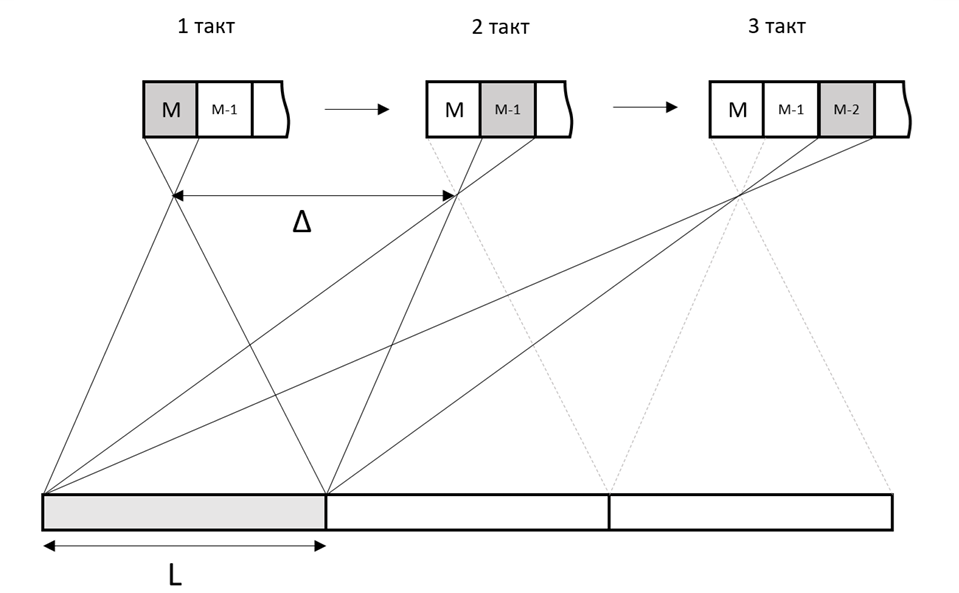
\includegraphics[scale=0.6]{VZN_opt}}
	\caption{Съёмка в режиме ВЗН без \blur{я} ($\tau_T = \tauopt{T}$) }
	\label{fig:VZN_opt}
\end{figure}


В случае, когда программно заданный тактовый период опроса $\tau_T$ оказывается больше оптимального значения $\tauopt{T}$, смещение за время одного такта становится меньше требуемого ($\Delta (\tau_T) < L $). В результате участок сцены проецируется одновременно на два соседних элемента ПЗС-матрицы, и в каждый такт накопления регистрируется сигнал не только от соответствующего участка сцены, но и от смежных областей изображения (Рисунок~\cref{fig:tauT_more}).

\begin{figure}[!h]
	\centerfloat{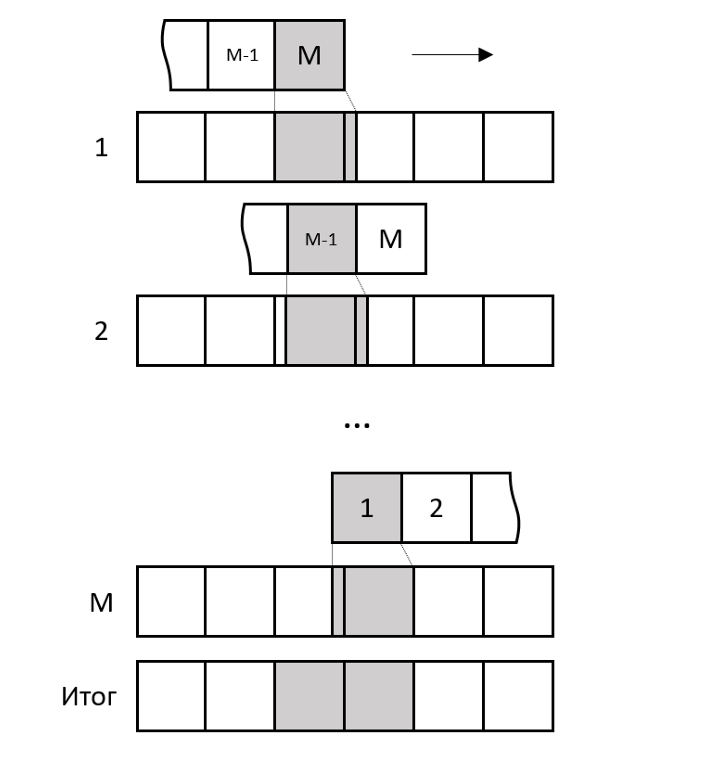
\includegraphics[scale=0.6]{tauT_more}}
	\caption{Возникновение \blur{я} при увеличенном тактовом периоде ($\tau_T > \tauopt{T}$) }
	\label{fig:tauT_more}
\end{figure}

Суммарная территория, участвующая в накоплении сигналов на каждом шаге, оказывается на $\frac{\delta}{M}\cdot L$ больше, чем при съёмке с оптимальным периодом опроса, где $\delta$ -- величина \blur{я} в элементах ПЗС-матрицы, $M$ -- число интеграционных шагов. Таким образом при $\tau_T > \tauopt{T}$ выражение~\eqref{eq:tau_noblur} примет вид:

\begin{equation}
	\label{eq:tau_more_blur}
		\Delta(\tau_T) = L \cdot \frac{(M+\delta)}{M}.
	\end{equation}

Аналогичная ситуация возникает в противоположном случае, когда заданный тактовый период меньше оптимального $\tau_T < \tauopt{T}$. В этом случае смещение изображения за один такт превышает допустимое $\Delta (\tau_T) > L$, и проекция участка сцены смещается быстрее, чем выполняется перенос зарядов. В каждый такт накопления регистрируется лишь часть сигнала от соответствующего участка, а оставшаяся информация теряется между проекциями (Рисунок~\cref{fig:tauT_less}).

\begin{figure}[!h]
	\centerfloat{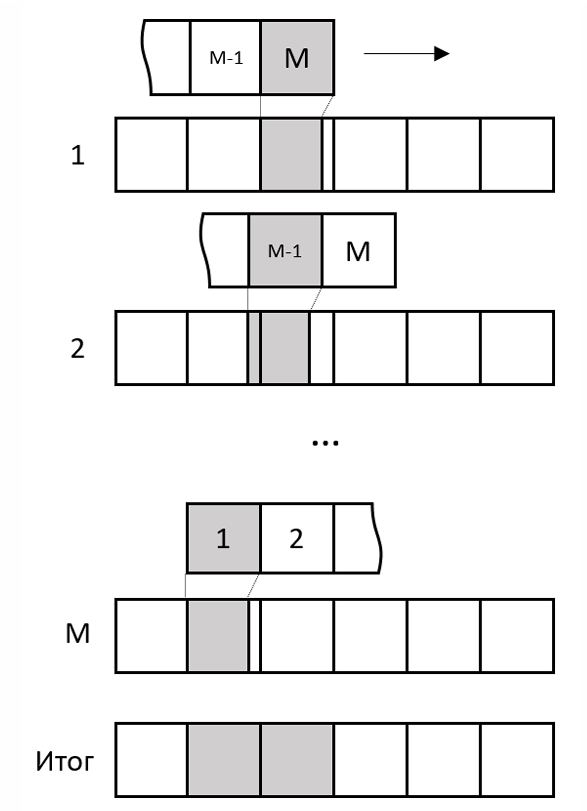
\includegraphics[scale=0.6]{tauT_less}}
	\caption{Возникновение \blur{я} при уменьшенном тактовом периоде ($\tau_T > \tauopt{T}$) }
	\label{fig:tauT_less}
\end{figure}

В результате изображение приобретает фрагментированный характер, снижается резкость и контрастность мелких деталей, выражение~\eqref{eq:tau_noblur} примет вид:
\begin{equation}
	\label{eq:tau_less_blur}
	\Delta(\tau_T) = L \cdot \frac{(M-\delta)}{M}.
\end{equation}

Оптимальный тактовый период опроса определяется по расчётной скорости движения изображения $v_0$:
\begin{equation}
	\label{eq:eq_optimalPeriod}
	\tau_T^* = \frac{L}{v_0} = \frac{l_x m_c}{v_0}.
\end{equation}


Практика эксплуатации показывает, что рассогласование между фактическим и расчётным тактовым периодом может быть вызвано целым комплексом факторов: методическими ошибками при расчёте скорости движения изображения, неточностью поддержания орбитальной и угловой ориентации, температурными деформациями конструкции и вибрациями. Наибольшее влияние в контексте данного исследования оказывают возмущения, возникающие при повороте подвижных частей оптической системы. Вращение оптической системы осуществляется моментом, формируемым приводом, который через механические связи передаёт на корпус космического аппарата реактивный момент. Под его действием изменяется угловая скорость КА, что ведёт к изменению скорости движения изображения на фокальной плоскости:

\begin{equation}
	\label{eq:eq_spdImgae}
	v=f\cdot \omega_{||},
\end{equation}

\noindent  где \(f\) "--- фокусное расстояние оптической системы, \(\omega_{||}\) "--- проекция угловой скорости на направление сканирования.

Изменение скорости изображения приводит к нарушению условия оптимального тактового периода $\tauopt{T}$, в результате чего проекция сцены смещается относительно матрицы приёмника и появляется \blur{е}. В терминах контрастно-частотной характеристики через множители $\text{КЧХ}_{LF}$ и $\text{КЧХ}_{HF}$ в выражении ~\eqref{eq:mtf_total}, которые отражают вклад низко- и высокочастотных колебаний.

Низкочастотные колебания являются наиболее критичным видом динамических возмущений, так как их амплитуда может достигать десятков микрометров, величины сравнимой с размером пикселя~\cite{Wahballah2018}.
В условиях, когда время экспозиции $\exposition$ существенно меньше периода колебаний $T_0$, \blur{е} формируется только на части синусоиды и приобретает квазилинейный характер. При этом величина \blur{я} становится случайной: она зависит от того, на какой фазе колебаний выполняется экспозиция. Минимальное размытие возникает, если экспозиция приходится на экстремум синусоиды, а максимальное  -- когда экспозиция совпадает с точкой нулевого перехода ~\cite{Haghshenas2015a} (рисунок ~\cref{fig:MTF_LF_phase}).

\begin{figure}[!h]
	\centerfloat{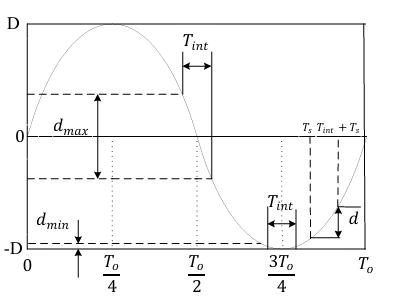
\includegraphics[scale=1]{mtf_lf}}
	\caption{Зависимость величины \blur{а} от фазы низкочастотных колебаний}
	\label{fig:MTF_LF_phase}
\end{figure}

Минимальный и максимальный радиусы \blur{я} определяются выражениями \eqref{blur_min}, \eqref{blur_max}

\begin{equation}
	\label{blur_min}
	d_{min} = D \left( 1 - \cos \left( \frac{2\pi}{T_0} \cdot \frac{T_{int}}{2} \right) \right),
\end{equation} 

\begin{equation}
	\label{blur_max}
	d_{max} = 2D \sin \left( \frac{2\pi}{T_0} \cdot \frac{T_{int}}{2} \right),
\end{equation}

\noindent  где \(D\) "--- амплитуда скорости колебаний, \(\exposition\) "--- время экспозиции, \(T_0\) "--- период колебаний.

Когда траектория смещения изображения в пределах кадра близка к линейной, снижение КЧХ описывается аппроксимацией линейного \blur{я}:

\begin{equation}
	\label{mtf_lf}
	\text{КЧХ}_{LF}(\nu)=\frac{\sin{\pi \nu L}}{\pi \nu L},
\end{equation}

\noindent  где \(L\) "--- величина смещения изображения за время экспозиции, \(\nu\) "--- пространственная частота.

Установлено, что низкочастотные колебания определяют предельное качество изображения. Например при увеличении амплитуды смещения с $1~\text{до}~20~\text{мкм}$ значение КЧХ на частоте Найквиста уменьшается на 41~\%, а при $30~\text{мкм}$ практически падает до нуля~\cite{wahballah2018smear}.

Высокочастотные колебания конструкции космического аппарата обычно возникают из-за дисбалансов реакционных маховиков, дефектов подшипников, работы приводов и упругих резонансов панелей. Характерный диапазон частот для таких возмущений составляет сотни герц и выше, а амплитуда смещений проекции изображения в фокальной плоскости, как правило, не превышает долей микрона (0,2–0,6~мкм) \cite{Haghshenas2015a}. Время экспозиции камеры существенно больше периода колебаний $\exposition \gg T_0$, поэтому результирующее смещение усредняется. 

Для гармонических высокочастотных колебаний КЧХ описывается через функцию Бесселя нулевого порядка:

\begin{equation}
	\label{eq:mtf_hf}
	\text{КЧХ}_{HF}(\nu)=J_0(2\pi \nu D).
	\end{equation}

При малых амплитудах ($D \ll p$, где \(p\)--размер пикселя) КЧХ $\approx 1$


В реальных условиях на движение изображения накладываются несколько высокочастотных гармоник. При суперпозиции двух синусоидальных гармоник итоговое значение КЧХ снижается сильнее, хотя деградация остаётся существенно меньше по сравнению с низкочастотными возмущениями.


В случае случайных высокочастотных колебаний, связанных с микродрожанием конструкции и шумами приводов, используется гауссова аппроксимация \cite{Holst2008}:

\begin{equation}
	\label{eq:mtf_rand}
	\text{КЧХ}_{HF}(\nu) = \exp\!\left(-2 \pi^2 \sigma_R^2 \nu^2 \right),
	\end{equation}

\noindent где \(\sigma_R\) "--- среднеквадратичное дрожание изображения.


Таким образом, высокочастотные вибрации вносят менее выраженный, но всё же значимый вклад в деградацию изображения. Их влияние становится критическим при совпадении спектра колебаний с резонансами конструктивных элементов КА или при наложении нескольких гармоник. Однако в большинстве практических сценариев $\text{КЧХ}_{HF}$ остаётся близкой к единице, а решающим ограничивающим фактором качества выступают низкочастотные колебания, описываемые через $\text{КЧХ}_{LF}$.

Характер воздействия реактивного момента на качество изображения можно условно разделить на три составляющих. Первая — низкочастотная, связанная с медленным изменением угловой скорости при выполнении манёвра. Она изменяет среднее значение скорости движения изображения, смещая систему из оптимального режима съёмки. Вторая — гармоническая, возникающая из-за колебаний элементов конструкции или резонансов в системе ориентации, которые могут поддерживаться вращающимися деталями исполнительных механизмов. Третья — случайная, обусловленная нерегулярными импульсами момента при работе приводов и механическими шумами. Все три компоненты вносят вклад в снижение функции передачи модуляции и интегральных показателей качества.

\section{Методы компенсации реактивного момента}
Возмущающий момент, возникающий при работе приводов подвижных частей космических аппаратов, является одним из ключевых факторов, ограничивающих точность наведения и стабилизации. Для снижения его влияния применяются различные методы компенсации, которые условно можно разделить на механические и алгоритмические. В основе большинства решений лежит идея создания дополнительного вращающегося или инерционного элемента, формирующего момент, противоположный возмущающему.

В мировой практике для компенсации реактивных моментов применяются различные технические и алгоритмические решения: использование реакционных маховиков и гиродинов \cite{pittelkau2012pointing, dennehy2021spacecraft}, балансировка подвижных узлов \cite{alvarez2018spacecraft}, а также специальные законы управления приводами, формирующие сглаженные профили разгона и торможения \cite{lappas2002attitude, zhao2023effect}. Дополнительно рассматриваются методы цифровой коррекции смаза на изображениях — геометрические, спектральные и градиентные, среди которых наиболее перспективными для реализации на борту являются градиентные подходы \cite{volobuev2021dissertation}. Эти меры позволяют снизить спектр возмущений в критически значимых диапазонах частот, однако минимизация их влияния на формируемое изображение остаётся актуальной задачей исследований.

Наиболее простым и широко используемым способом является применение компенсирующего маховика, вращающегося во встречном направлении относительно основного привода. При этом создаётся противодействующий момент, позволяющий снизить суммарное воздействие на основание конструкции. Правильный подбор инерционных характеристик маховика обеспечивает уменьшение низкочастотной составляющей возмущений, возникающих при разгоне и торможении нагрузки, а также частичную компенсацию гармонических возмущений. Подобная схема используется в системах наведения оптических приборов и антенн, где требуется высокая точность удержания линии визирования \cite{montenbruck2002satellite}. Ограничением метода является необходимость размещения дополнительного узла и обеспечения его синхронной работы с основным приводом, что увеличивает массу, энергопотребление и сложность управления.

Другим конструктивным решением является использование двухприводных систем. В этом случае нагрузка перемещается с помощью двух двигателей, установленных симметрично относительно центра масс. Каждый двигатель создаёт собственный реактивный момент, но благодаря зеркальному расположению и синхронизации вращения они взаимно компенсируются. Такой подход снижает передачу возмущений на корпус аппарата и уменьшает требования к жёсткости несущей конструкции. Применение двухприводных схем было предложено в ряде исследовательских проектов для систем наведения антенн и высокоточных зеркальных механизмов \cite{worthington2010design}. Недостатком является усложнение системы управления, необходимость точного согласования работы приводов и усложнение конструкции.

Одним из оригинальных инженерных решений, направленных на исключение передачи возмущающего момента на корпус космического аппарата, являются приводы с подвижным статором. В таких конструкциях статор двигателя не жёстко закреплён, а установлен на подшипниках и может свободно поворачиваться вокруг оси ротора. Реактивный момент, возникающий при работе ротора, приводит к вращению статора, который через редуктор или напрямую соединён с маховиком-компенсатором. Последний создаёт уравновешивающий момент, противоположный по направлению к моменту от ротора. Таким образом достигается полное исключение передачи реактивного момента на основание. Питание обмоток статора осуществляется через скользящие токоподводы, что усложняет конструкцию, но позволяет реализовать компактный узел с высокой степенью компенсации возмущений~\cite{RU2646002C2}. Другим направлением развития являются двигательные приводы с редукторами, применяемые, в частности, для наведения антенн и солнечных батарей. В патенте~\cite{RU2466069C2} описана конструкция электропривода с редуктором, обеспечивающая высокую долговечность и точность позиционирования за счёт применения гармонического или планетарного редуктора в сочетании с преднатянутыми подшипниками. Такая схема позволяет минимизировать люфты и компенсировать тепловые деформации в условиях длительной работы в космосе. Основным эффектом является значительное снижение передачи вибраций и случайных колебаний на корпус аппарата при сохранении высокого крутящего момента на выходе редуктора.

Важным направлением во всех описанных приводах является использование балансировочных устройств, которые позволяют уменьшить динамические возмущения за счёт устранения эксцентриситета и неидеальной балансировки роторов. Для этого на подвижные элементы устанавливаются специальные балансировочные грузы или кольца, компенсирующие смещение центра масс. Такой подход позволяет эффективно снизить как гармонические, так и случайные составляющие возмущающего момента. Особенно актуальны эти меры в системах с быстро вращающимися деталями, где даже незначительный дисбаланс приводит к формированию высокочастотных вибраций, передающихся на корпус и ухудшающих характеристики оптико-электронной аппаратуры. В ряде работ продемонстрировано, что правильно подобранные балансировочные элементы способны существенно уменьшить уровень микровибраций \cite{liu2008reaction,alcorn2018fully}. Ограничением метода является то, что он в основном устраняет статические и динамические дисбалансы, но не способен компенсировать момент, возникающий непосредственно от управляющих воздействий на привод.

Помимо конструктивных решений, активно развиваются алгоритмические методы компенсации. Их суть заключается в формировании такого закона управления приводом, при котором динамические возмущения минимальны. Наиболее известными являются S-образные, синусоидальные и другие сглаженные профили ускорения, которые ограничивают спектр возбуждаемых гармоник и предотвращают возникновение резонансов в конструкции. Алгоритмическая компенсация особенно эффективна для снижения случайной составляющей реактивного момента, обусловленной нерегулярными импульсами момента при работе привода и механическими шумами. В публикации \cite{singer1990preshaping,singhose2009command} показано, что правильно выбранный профиль управления позволяет существенно снизить остаточные возмущения без введения дополнительных механических элементов, что делает метод перспективным для лёгких и маломощных космических аппаратов. Однако его эффективность зависит от точности модели системы и качества обратной связи, поэтому в реальных условиях полного устранения возмущений добиться не удаётся.

Таким образом, существующие методы компенсации реактивного момента охватывают широкий спектр решений: от введения дополнительных механических узлов до оптимизации управляющих воздействий. Каждое из них имеет свои преимущества и ограничения. Наиболее эффективной на практике является комбинация механических и алгоритмических средств, обеспечивающая одновременное снижение как низкочастотной и гармонической составляющих, так и случайных возмущений. Однако вследствие технологических и конструктивных ограничений полностью устранить воздействие не удаётся, и в системе всегда остаётся остаточный реактивный момент, который подлежит регистрации и последующей оценке.


\subsection{Компенсация реактивного момента}

Для компенсации реактивного момента, возникающего при разгоне и торможении инерционных объектов (зеркал, оптических сборок и др.), может применяться активная электромеханическая схема с соосным компенсирующим приводом. Принципиальная идея заключается в установке второго ротора с динамикой, противоположной по направлению основной нагрузке. При равенстве динамических моментов обоих приводов результирующее воздействие на корпус спутника обращается в ноль:

\begin{equation}
	\label{eq:equal_inertia}
	J_1\frac{d\omega_1}{dt}+J_2\frac{d\omega_2}{dt} = 0,
\end{equation}


\noindent где \(J_1,J_2\)"--- моменты инерции подвижных частей, \(\omega_1,\omega_2\)"--- угловые скорости.

На практике конфигурация может быть реализована как с двумя независимыми двигателями, так и с использованием редукторной связи между основным и компенсирующим ротором. Применение редуктора позволяет снизить массу маховика, так как эквивалентный момент инерции уменьшается пропорционально квадрату коэффициента передачи $i$.

Особое внимание при проектировании систем компенсации реактивного момента уделяется трению в шарикоподшипниках, которое в условиях космоса становится главным источником сопротивления. Даже при отсутствии атмосферы и силы тяжести момент трения сохраняется за счёт предварительного натяга, центробежных и гироскопических сил. Проблема точной оценки момента трения особенно важна при разработке приводов оптико-механических систем, где остаточный реактивный момент напрямую влияет на качество изображения. В ряде работ~\cite{Babaeva1962, Delektorskii1968, Shashanov1971,Yavlensky1981} отмечено, что суммарный момент $M_{\text{тр}}$ в подшипниках включает две основные составляющие: момент трения от нагрузки $M_0$ и гидродинамическую составляющую смазки $M_1$. При этом именно $M_1$ во многих случаях оказывается доминирующим~\cite{Mikhailov2014}. Для количественной оценки момента трения в радиально-упорных шарикоподшипниках изделий космического назначения используются уточнённые эмпирические зависимости. Согласно работе~\cite{Delektorskii1968}, суммарный момент трения может быть представлен следующим образом:

\begin{equation}
	\label{eq:Mtr}
	M_{\text{тр}} = M_0 + M_1 = 0{,}6 \cdot 10^{-3} A_0
	\frac{D_0}{d_{\text{ш}}} \cdot \frac{1}{\sqrt[3]{z d_{\text{ш}}}}+4{,}41 \cdot 10^{-6} \cdot D_0^3 n,
\end{equation}
где \(A_0\)"--- осевой преднатяг, \(D_0\)"--- средний диаметр подшипника, \(d_{\text{ш}}\)"--- диаметр шарика, \(z\)"--- число шариков, \(n\)"--- скорость вращения.
	
Формула (\ref{eq:Mtr}) даёт удовлетворительное совпадение с экспериментальными данными (погрешность не превышает 20 \%), что позволяет использовать её для инженерных расчётов при проектировании приводов и маховиков в космических аппаратах.

Характерным является наличие момента трогания $M_{\text{трог}}$, который превышает установившийся момент сопротивления в среднем в $1,5-2$ раза~\cite{Mikhailov2014}. Это приводит к скачкообразной передаче момента на корпус спутника в момент пуска. При несовпадении значений $M_{\text{трог}}$ у основного и компенсирующего приводов возникает остаточное возмущение, вызывающее угловой дрейф. Для снижения влияния момента трогания применяются конструктивные и технологические меры. Наиболее распространённым методом является предварительная обкатка подшипников, позволяющая снизить $M_{\text{трог}}$ в 2–3 раза и повысить стабильность его значения во времени~\cite{Mikhailov2014}. Существенное влияние оказывает выбор смазки: использование консистентных смазок с оптимальной вязкостью позволяет уменьшить разброс значений момента трогания между подшипниками. Важным является и обеспечение высокой точности обработки дорожек качения, что снижает локальные пики сопротивления при запуске.Со стороны систем управления эффект момента трогания компенсируется формированием специальных профилей разгона с контролируемым нарастанием момента. Это позволяет синхронизировать работу основного и компенсирующего приводов и уменьшить риск возникновения остаточного момента.

Однако, даже при использовании соосных компенсирующих приводов и учёте особенностей трения в подшипниках полностью устранить остаточный реактивный момент не удаётся. Его величина определяется как конструктивными факторами (точность изготовления, свойства смазки, качество сборки), так и алгоритмами управления приводами. Поэтому для корректной оценки влияния возмущающих моментов на динамику космического аппарата необходимо не только их моделирование, но и прямые экспериментальные измерения.

\section{Измерение реактивного момента}


С точки зрения механики сплошных сред, крутящий момент можно определить как произведение силы на плечо её приложения:

\begin{equation}
	\label{eq:eq_Torque}
	M=F \cdot r,
\end{equation}
где \(F\) "--- приложенная сила, \(r\) "--- расстояние от точки приложения силы до оси вращения.

Для вала круглого сечения при кручении момент связан с углом закручивания $\phi$ выражением:

\begin{equation}
	\label{eq:eq_torque}
	M=G\cdot J \cdot \frac{\phi}{L},
\end{equation}
где \(G\) "--- модуль сдвига материала, \(J\) "--- полярный момент инерции сечения, \(L\) --- длина участка.

Именно эта зависимость лежит в основе многих методов измерения момента -- фиксируется угол закручивания или напряжённое состояние материала, а затем по известным параметрами конструкции вычисляется величина момента.

Современные датчики крутящего момента реализуются на основе более чем десяти различных физических принципов. Наиболее распространённые из них:
\begin{itemize}
	\item Тензорные датчики -- основаны на измерении деформации упругого элемента с помощью тензорезисторов. Отличаются высокой точностью, но требуют установки датчика в разрыв вала\cite{yeh2015digital,Hou2009,Mohammed2008,Chen2020}.
	\item магнито-упругие -- используют эффект изменения магнитной проницаемости материала под действием кручения. Недостаток -- чувствительны к внешним полям \cite{Shu2007}.
	\item Оптоволоконные датчики с решётками Брэгга -- фиксируют микродеформации с высоким разрешением, однако требуют намотки волокна на вал и потому не являются полностью бесконтактными \cite{Zhu2021}
	\item Пьезоэлектрические и фотоупругие датчики -- преобразуют механическую деформацию в электрический сигнал, могут быть миниатюрных размеров, но ограничены по диапазону измерения \cite{Bojtos2017,Hu2020}.
	\item Оптические методы -- обеспечивают бесконтактность и высокую точность, но подвержены влиянию вибрации \cite{Garinei2017,Sjodahl1996}
\end{itemize}
Несмотря на разнообразие подходов, все методы делятся на две большие категории:
\begin{itemize}
	\item Контактные датчики -- взаимодействуют с объектом напрямую, интегрируются в конструкцию. Они обеспечивают высокое качество измерений, но изменяют характеристики самой системы.
	\item Бесконтактные датчики -- не оказывают механического воздействия, удобны для встроенного мониторинга, но ограничены по разрешению и устойчивости к возмущениям \cite{Wang2021}. 	
\end{itemize} 

Контактные методы применимы для широкого диапазона задач, но в высокоточных системах (робототехника, аэрокосмические приводы, микро-механизмы) критично минимизировать их влияние на конструкцию. Бесконтактные оптические методы обладают рядом преимуществ: высокой точностью, нечувствительностью к температурным и электромагнитным помехам, малым влиянием на исследуемую систему. Однако они традиционно сталкиваются с проблемой устойчивости к радиальным вибрациям и ограничениями по диапазону.

В качестве примера современных тенденций в этой области можно привести исследование \cite{Chen2024}, где предложен новый бесконтактный метод измерения момента, основанный на оптической когерентной интерферометрии. Принцип заключается в нанесении микрошкал на поверхность вала (ширина порядка 62,8 мкм), которые служат физической картой деформаций. Оптическая система регистрирует смещения шкал при закручивании вала, а специальные алгоритмы обработки сигнала (быстрое преобразование Фурье и метод энергетического центра Ханнинга) обеспечивают разрешение вплоть до 0,003 Н·м. Несмотря на то, что данный метод не используется в рамках настоящей работы, он иллюстрирует направление развития современных бесконтактных технологий измерения момента.

Большинство существующих методов ориентировано на измерение момента непосредственно в точке приложения привода, то есть на его валу. В отличие от локального крутящего момента, который характеризует работу конкретного исполнительного узла и фиксируется в месте передачи энергии, реактивный момент проявляется как отклик на основании или несущей конструкции и отражает интегральное воздействие привода на систему в целом. В космических приложениях ключевым становится именно измерение реактивного момента, так как он определяет динамические возмущения, передающиеся на корпус аппарата и влияющие на точность ориентации в пространстве.

Для снижения возмущений реактивный момент обычно компенсируется с помощью дополнительного маховика, вращающегося в противоположном направлении. Однако компенсация никогда не является полной: вследствие несовершенства балансировки и нелинейностей в системе остаётся остаточный реактивный момент. Его регистрация и количественная оценка необходимы для анализа устойчивости системы и корректного прогнозирования влияния привода на работу всего аппарата.

В доступной литературе практически отсутствуют исследования, посвящённые детальному расчёту и, в особенности, непосредственному измерению реактивного момента, возникающего при вращении подвижных частей оптико-электронной аппаратуры космического назначения. В немногочисленных публикациях, где рассматривается вопрос измерений, регистрация реактивного момента, как правило, осуществляется на валу привода или двигателя \cite{Rayanov2020}, что отражает лишь локальное крутильное воздействие в месте установки датчика. Однако такой подход не позволяет получить эквивалентный полный вектор реактивного момента, передаваемого на корпус космического аппарата, поскольку не учитываются дополнительные компоненты, возникающие вследствие смещений центра масс, инерционного взаимодействия подвижного узла с несущими элементами конструкции, а также динамических эффектов в механизмах передачи движения. Наиболее близким по постановке задачи к настоящему исследованию является метод определения возмущающего момента, реализованный на инерционном стенде для экспериментальной отработки системы наведения антенн космического аппарата \cite{Goncharuk2013}. Рассмотрим этот метод подробнее. Конструкция стенда представлена на рисунке ~\cref{fig:stand}.
\begin{figure}[ht] 
	\centerfloat{
		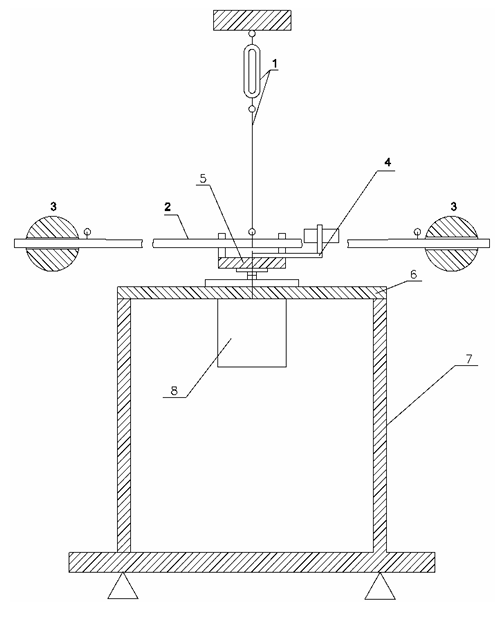
\includegraphics[scale=0.8]{stand} 
	}
	\legend{1 – система обезвешивания; 2 – штанга; 3 – груз; 4 – датчик угловой скорости с кронштейном для установки; 5 – элемент для передачи момента на выходной вал; 6 – плита установочная; 7 – основание; 8 – объект контроля}
	\caption{Функциональная схема инерционного стенда}
	\label{fig:stand} 
\end{figure}

Метод определения возмущающего момента, реализованный в рассмотренной работе, %todo переписать соавторов
основан на использовании инерционного стенда, позволяющего воспроизводить динамические характеристики системы наведения антенн космического аппарата в наземных условиях. Конструктивно стенд представляет собой основание с закреплённой на нём плитой, на которой устанавливается механический привод антенны. К выходному валу привода присоединяется имитатор нагрузки, выполненный в виде штанги с грузами, масса и положение которых подбираются таким образом, чтобы эквивалентный момент инерции соответствовал параметрам реальной антенны. Для снижения влияния силы тяжести используется система обезвешивания, а инерционный имитатор позволяет воспроизводить упругие и динамические свойства навешиваемого оборудования. Регистрация параметров движения осуществляется с помощью датчика угловой скорости, установленного непосредственно на выходном валу привода. В процессе эксперимента фиксируется изменение угловой скорости при различных режимах работы — как при равномерном вращении, так и в переходных процессах разгона и торможения. Полученные зависимости $\omega(t)$ подвергаются дифференцированию для вычисления углового ускорения, после чего возмущающий момент определяется по выражению:
\begin{equation}
	\label{eq:eq_M_disturb}
	M=J_{\text{н}}\cdot \frac{d\omega}{dt},
\end{equation}
где \(J_{\text{н}}\) "--- момент инерции имитируемой нагрузки, \(\omega\) "--- угловая скорость.

Таким образом, метод сводится к регистрации динамики вращения исполнительного механизма и последующему вычислению возмущающего момента через известные параметры имитируемой нагрузки.

Применение данного метода позволяет оценить возмущающее воздействие, создаваемое приводом в установившихся и переходных режимах, а также проанализировать их спектральные характеристики.

Несмотря на несомненные достоинства, описанный метод имеет ряд ограничений, которые не позволяют использовать его в рамках настоящего исследования. Прежде всего следует отметить, что стенд оперирует не реальной нагрузкой, а её имитатором, выполненным в виде штанги с грузами. Для каждой конкретной аппаратуры требуется изготавливать отдельный имитатор с заданным моментом инерции, и даже при тщательной калибровке всегда сохраняется погрешность в воспроизведении динамических характеристик реального узла. Кроме того, сам принцип измерений остаётся локальным: возмущающий момент определяется по данным датчика, установленного на валу привода, тогда как для задач космической техники критическим является именно реактивный момент, передаваемый на корпус КА. Такой подход не позволяет получить полное представление о суммарном воздействии на конструкцию в реальных условиях работы. Наконец, существенным ограничением является невозможность воспроизведения ситуации, когда одновременно вращаются и нагрузка, и компенсирующий маховик. Регистрация реактивного момента после компенсации имеет принципиальное значение для оценки качества динамики в высокоточных оптико-электронных системах. В совокупности, эти факторы делают метод, реализованный на инерциальном стенде, недостаточным для решения поставленной в настоящей работе проблемы.

\section*{Выводы по главе 1}
В первой главе рассмотрено современное состояние исследований в области динамических воздействий на оптико-электронные системы космических аппаратов и их влияние на качество формируемых изображений. Показано, что повышение разрешающей способности и внедрение механизмов поворота визирной оси без разворота аппарата сопровождается ростом требований к стабилизации изображения и одновременно приводит к усилению динамических возмущений, вызванных перемещением подвижных масс.

Анализ показал, что реактивный момент, возникающий в результате работы приводов, является одним из ключевых факторов, снижающих качество изображений. Его влияние проявляется через три компоненты: низкочастотную, гармоническую и случайную. Все они приводят к смещению скорости движения изображения на фокальной плоскости относительно оптимального значения, что вызывает \blur{е} и дрожание изображения, а также снижает интегральные показатели качества, включая КЧХ и Image Quality Factor.

Для снижения воздействия реактивного момента применяются различные методы компенсации, включая компенсирующие маховики, двухприводные механизмы, балансировочные устройства и алгоритмическую компенсацию на уровне законов управления. Эти решения позволяют уменьшить спектр возмущений в критических диапазонах частот, однако полностью устранить их влияние не удаётся. В системе неизбежно остаётся остаточный реактивный момент, который требует учёта и оценки.

Обзор существующих методов измерения крутящего момента показал, что они в основном ориентированы на регистрацию момента на валу двигателя. Такой подход отражает только локальное крутильное воздействие и не эквивалентен реактивному моменту, передаваемому на корпус космического аппарата. Рассмотренный метод экспериментальной отработки на инерционном стенде позволяет оценить возмущающие моменты привода, однако он основан на использовании имитатора нагрузки и не учитывает работу компенсирующих маховиков, а потому не позволяет регистрировать остаточный реактивный момент всей системы.

Таким образом, выполненный анализ подтвердил, что в доступной литературе практически отсутствуют исследования, посвящённые непосредственному измерению реактивного момента подвижных частей оптико-электронной аппаратуры космического назначения. Этот пробел обосновывает необходимость разработки специализированных методов регистрации и анализа остаточного реактивного момента, что и составляет предмет настоящего исследования.

\FloatBarrier

           % Глава 1
\chapter{Анализ влияния алгоритма управления приводами СПН и кинематической погрешности привода на величину некомпенсировааных моментов, возникающих при перенацеливании}\label{ch:ch2}

\section{Синусоидальный алгоритм управления}\label{sec:ch2/sec1}

Рассмотрим алгоритм управления при котором угловое ускорения привода меняется по закону синуса:

\begin{samepage}
	\begin{equation}
		\label{eq:eqCh2_sin}
		\begin{aligned}
			\epsilon = U \cdot \sin(f \cdot t)
		\end{aligned}	
	\end{equation}
	
	\begin{align*}
		\text{где} \quad 
		& U \text{ — амплитуда ускорения, в } \text{рад/с}, \\           
		& f = \frac{2 \cdot \pi}{T} \text{ — круговая частота}, \\       
		& T \text{ — период перенацеливания.}
	\end{align*}
\end{samepage}
	
Тогда, интегрируя это выражение, получим для угловой скорости:
\begin{equation}
	\label{eq:eqCh2_sinIntegral}
	\Omega = \left(1 - \cos\left(f \cdot t\right)\right) \cdot \frac{U}{f} \quad \si{\radian\second}
\end{equation}

Проинтегрировав ещё раз - получим выражение для угла поворота:
\begin{equation}
	\label{eq:eqCh2_sinIntegral2}
	\phi = \left( \frac{t}{f} - \sin\left(f \cdot t\right) \right) \cdot \frac{U}{f^2} \si{\radian}
\end{equation}

Из условия, что время перемещения подвижной части $T = 4 \si{\sec}$, угол поворота выходного вала равен $\phi = \SI{17}{\degree} = \SI{0.297}{\radian}$.
Из уравнения ~\cref{eq:eqCh2_sinIntegral2} получим:

\begin{equation}
	\label{eq:eqCh2_Uacc}
	U = \frac{\phi \cdot f^2}{t - \sin(f \cdot t)}
\end{equation}

Подставив числовые данные, получим:$U = 0{,}1832\,\si{\radian/ \second^2}$, $f = \pi/2$.




На рисунке~\cref{fig:sin_profile} приведены графики зависимостей угла, скорости и ускорения от времени. Управление приводом производится по закону:
\[
\Omega(t) = \left( 1 - \cos \left(f \cdot t \right)\right) \cdot \frac{U}{f}, \quad \si{\radian\per\second}.
\]

\begin{figure}[ht]
	\centerfloat{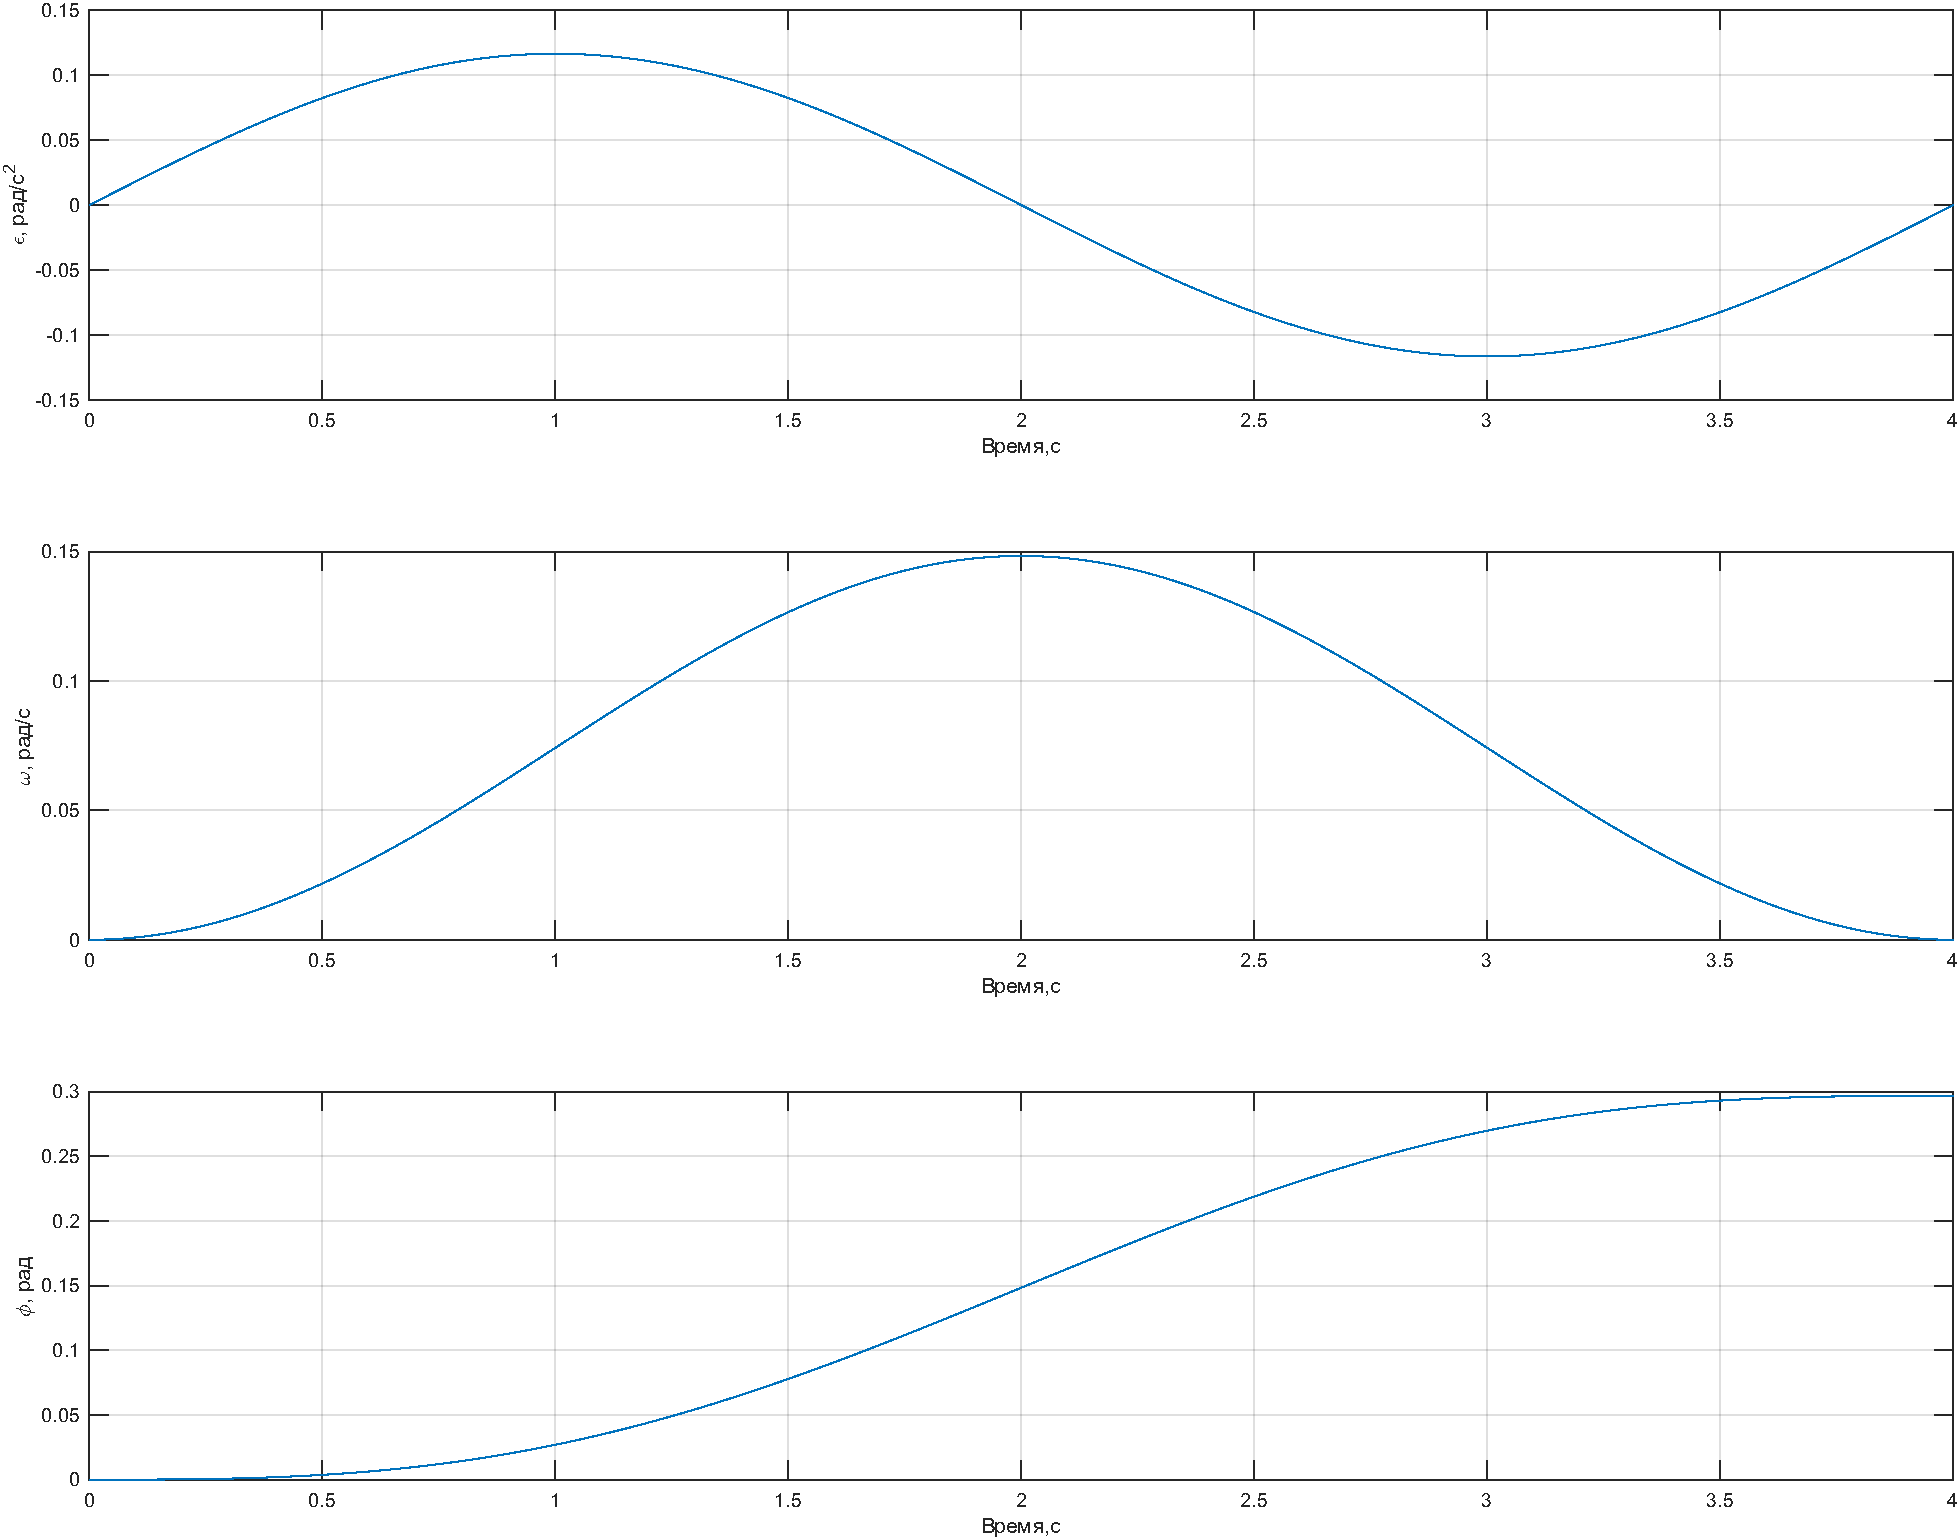
\includegraphics[scale=0.7]{matlab/sin_profile.pdf}}
	\caption{Зависимость углового ускорения, скорости и углового положения от времени}
	\label{fig:sin_profile}
\end{figure}


Таким образом, для задания закона управления приводом достаточно задать значения угла поворота~$\phi$ и времени перемещения~$T$.

На рисунке~\cref{fig:sin_moment} представлен график реактивного момента на основание при моменте инерции блока зеркал $J_m = \SI{2.96}{\kilogram\metre\squared}$.

\begin{figure}[ht]
	\centerfloat{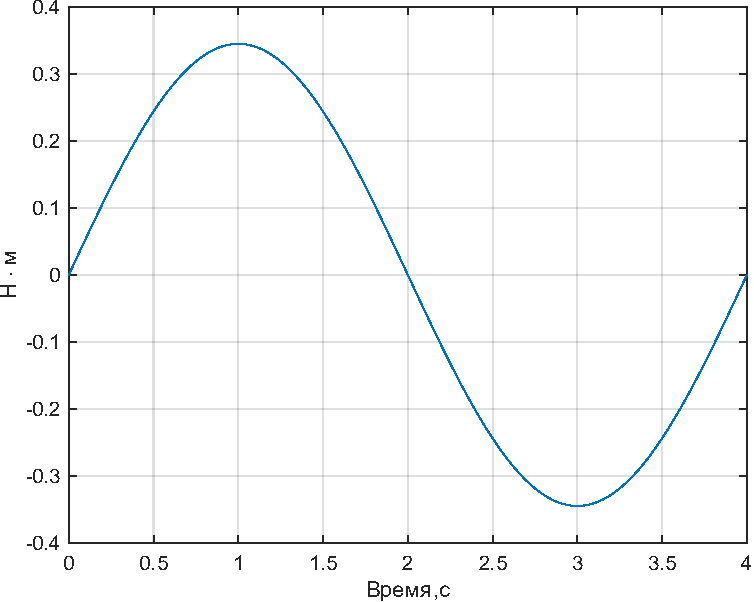
\includegraphics[scale=0.7]{matlab/sin_moment.pdf}}
	\caption{Реактивный момент при синусоидальном профиле разгона}
	\label{fig:sin_moment}
\end{figure}

Из графика видно, что максимальный реактивный момент на основание космического аппарата достигает значения~ $M = J_m \cdot \epsilon = \SI{0.35}{\newton\metre}.$ Момент имеет круговую частоту $f = \frac{\pi}{2}\, \si{\radian/\second}$, что соответствует частоте~\SI{0.25}{\hertz}. Эта частота близка к частотам собственных колебаний космического аппарата: \SI{0.2}{\hertz} по координате~$Z$ и \SI{0.174}{\hertz} по координате~$Y$. Указанное обстоятельство, при плохой настройке маховика и значительных остаточных моментах, может привести к возбуждению колебаний КА по этим осям.

\section{Линейный алгоритм управления}\label{sec:ch2/sec2}

Рассмотрим теперь алгоритм управления по линейному закону.

\begin{figure}[ht]
	\centerfloat{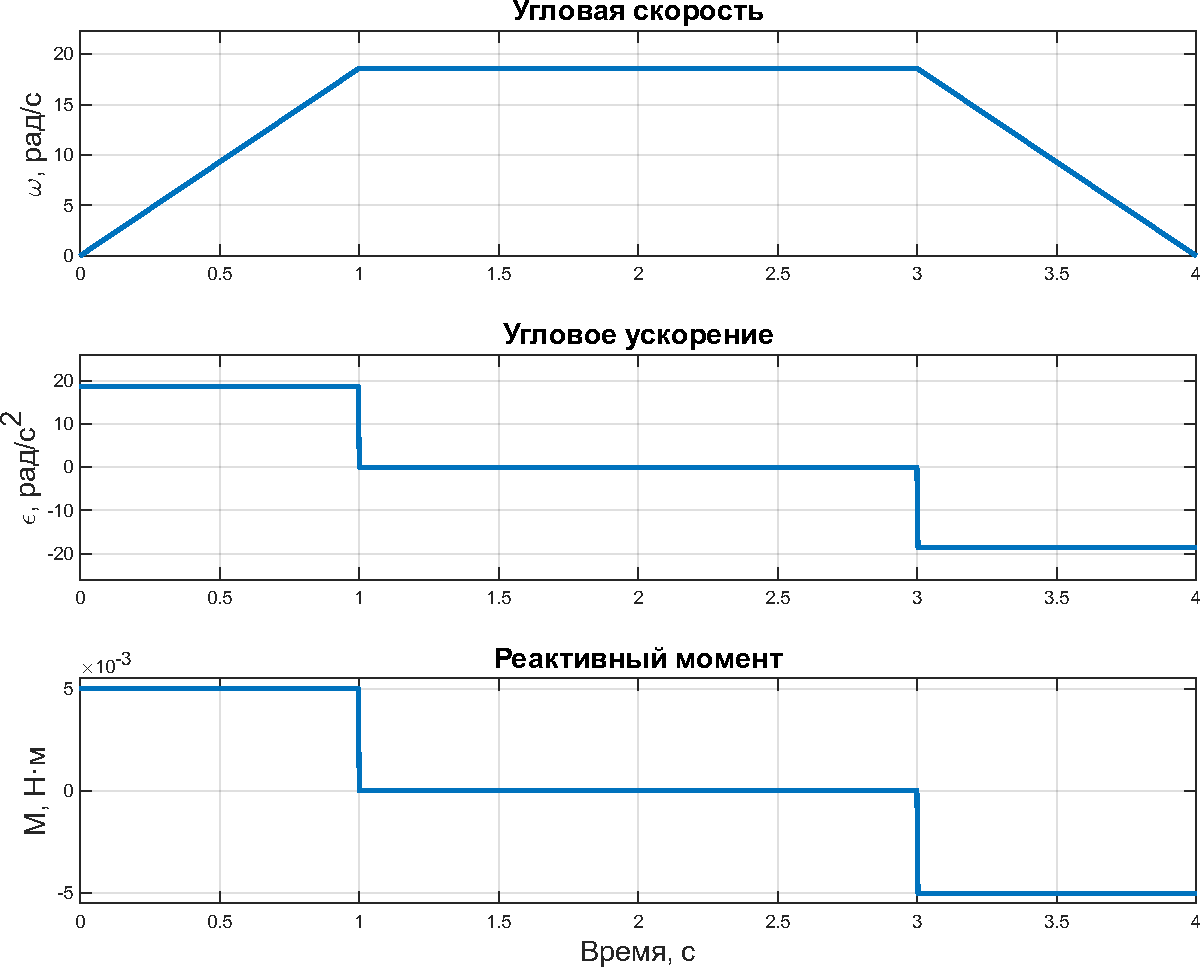
\includegraphics[scale=0.7]{matlab/line_profile.pdf}}
	\caption{Зависимость углового ускорения, скорости и углового положения от времени при линейном профиле разгона}
	\label{fig:line_profile}
\end{figure}

На рисунке~\cref{fig:line_profile} представлен упрощённый график изменения угловой скорости вращения и углового ускорения блока зеркал при перенацеливании на угол 17°. В течение времени разгона $t_a$ происходит увеличение скорости привода СПН, затем в течение $t_n$ происходит  движение с максимальной скоростью, и за время $t_d$ происходит торможение привода. В соответствии с ТЗ весь процесс должен занимать 4 с. Тогда можно записать:

\begin{equation}
	\label{eq:eqCh2_t_move}
	t_a+t_m+t_d=\SI{4}{\second}
\end{equation}

С другой стороны, за это время блок зеркал должен повернуться на угол 17°. Обозначим максимальную скорость $\omega_{nom}$, тогда для угла поворота получим:

\begin{equation}
	\label{eq:eqCh2_t_acc}
	\phi = t_a \cdot \frac{\omega_{nom}}{2} + t_n \cdot \omega_{nom} + t_d \cdot \frac{\omega_{nom}}{2} = \SI{17}{\degree}
\end{equation}

Номинальная скорость определяется из условия, что нужно преодолеть \SI{17}{\degree} за \SI{4}{\second}.
\begin{align*}
	t_a &= t_d = \SI{1}{\second}, \\
	t_n &= \SI{2}{\second}
\end{align*}
Тогда номинальная скорость определяется следующим образом:
\[
\omega_{nom} = \phi / 3 = 0,2967/3 = \SI{0.0989}{\radian/\second} 
\]
Максимальная частота управляющих сигналов для используемого в приводах шагового электродвигателя составляет 500 Гц. Одному периоду сигнала соответствует поворот ротора на угол 1,8°. Таким образом, максимальная скорость вращения шагового электродвигателя составит $\Omega_{d} = 500 \cdot 1,8 = \SI{900} {\degree/ \second}$. Максимальная угловая скорость блока зеркал составит $\Omega_{max}= 900/160 = \SI{5,625}{\degree/ \second}$. Подставим это значение в полученные выше уравнения~\cref{eq:eqCh2_t_move}и~\cref{eq:eqCh2_t_acc} и решим их совместно. Получим:


Отсюда ускорение разгона $\omega_{nom} / t_a = \SI{5,22}{\degree/\second\square} = \SI{0,091}{\radian/\second\square}$


Максимальный (без компенсации маховиками) реактивный момент для момента инерции блока зеркал $J_m = \SI{2,96}{\kilogram\cdot\meter\square}$ будет \mbox{\SI{0,091}{\radian / \second\square}  $\cdot 2,96 = \SI{0,269}{\newton\meter}$}.

Пусть:
\begin{align*}
	t_a &= t_d = \SI{2,05}{\second}, \\
	t_m &= \SI{0}{\second}
\end{align*}

Средняя скорость для выполнения перенацеливания на \SI{17}{\degree}
за \SI{4}{\second} составит $\Omega_{cp} = 17 / 4 = \SI{4,25}{\degree / \second}$. При движении по симметричному треугольному алгоритму ускорение разгона составит $\Omega_{cp} / t_p = \SI{2,024}{\degree / \second\square} = \SI{0,035}{\radian / \second\square}$, тогда максимальный (без компенсации маховиками) реактивный момент для момента инерции зеркал $J_m = \SI{2,96}{\kilogram \cdot \meter\square}$ составит $0,035 \cdot 2,96 = \SI{0,1}{\newton\meter}$

Таким образом, используя линейный треугольный закон разгона-торможения можно снизить реактивный момент на основание в 2,5 раза, что существенно облегчает задачу компенсации реактивного момента.

Следует отметить, что линейный график углового перемещения узла зеркал даёт несколько меньше (по сравнению с синусоидальным законом управления) постоянное значение ускорения (и, соответственно, реактивного момента) на участках разгона и торможения. Таким образом подбирая закон разгона и торможения можно управлять значением реактивного момента.

\section{Экспоненциальный алгоритм управления}\label{sec:ch2/sec3}

Особенности использования шагового электродвигателя со значительной инерционной нагрузкой обуславливают необходимость осуществления его разгона и торможения по определённому закону с плавными изменениями параметров движения. Это позволяет минимизировать вероятность потери шагов, снизить вибрации и обеспечить устойчивую работу привода.

В качестве примера такого закона может быть использована кусочно-заданная функция угловой скорости, включающая три стадии: экспоненциальный разгон, равномерное движение с номинальной скоростью и плавное экспоненциальное торможение. Данный закон описывается следующими выражениями:

\begin{samepage}
\begin{equation}
	\label{eq:expOmega}
	\omega(t) =
	\begin{cases}
		\omega_{\min} + (\omega_{\max} - \omega_{\min}) \cdot \left(1 - e^{-k t} \right),
		& 0 \leq t < t_r \\
		\omega_{\max}, 
		& t_r \leq t < t_r + t_c \\
		\omega_{\min} + (\omega_{\max} - \omega_{\min}) \cdot e^{-k (t - t_r - t_c)},
		& t_r + t_c \leq t \leq T
	\end{cases}
\end{equation}

где: \\
\quad $t$ — время движения; \\
\quad $\Omega(t)$ — угловая скорость во времени; \\
\quad $\Omega_{\min}$, $\Omega_{\max}$ — минимальная и максимальная скорость; \\
\quad $t_a$ — время разгона; \\
\quad $t_n$ — время равномерного движения; \\
\quad $T = 2t_a + t_n$ — общее время движения; \\
\quad $k$ — коэффициент плавности экспоненциального изменения.
\end{samepage}


На рисунке~\ref{fig:exp_profile} приведена характерная S-образная кривая скорости привода, построенная по вышеуказанной формуле. Кривая включает плавный экспоненциальный разгон, участок движения с постоянной скоростью и плавное экспоненциальное торможение.

График построен для случая движения со следующими параметрами: \\
\quad $\Omega_{\max} = 5{,}6^\circ/\text{с}$, \\
\quad $\Omega_{\min} = 0{,}02^\circ/\text{с}$, \\
\quad $k = 4$, \\
\quad $t_r = 1$ с — время разгона, \\
\quad $t_c = 2$ с — время равномерного движения. \\

Использование данной функции позволяет достичь необходимой скорости за ограниченное время с минимальными динамическими нагрузками, что особенно важно при работе с механизмами, обладающими значительным моментом инерции. Кусочно-заданный характер функции обеспечивает плавность переходов между стадиями движения и исключает резкие изменения ускорения, типичные для линейных или трапецеидальных профилей.

\begin{figure}[ht]
	\centerfloat{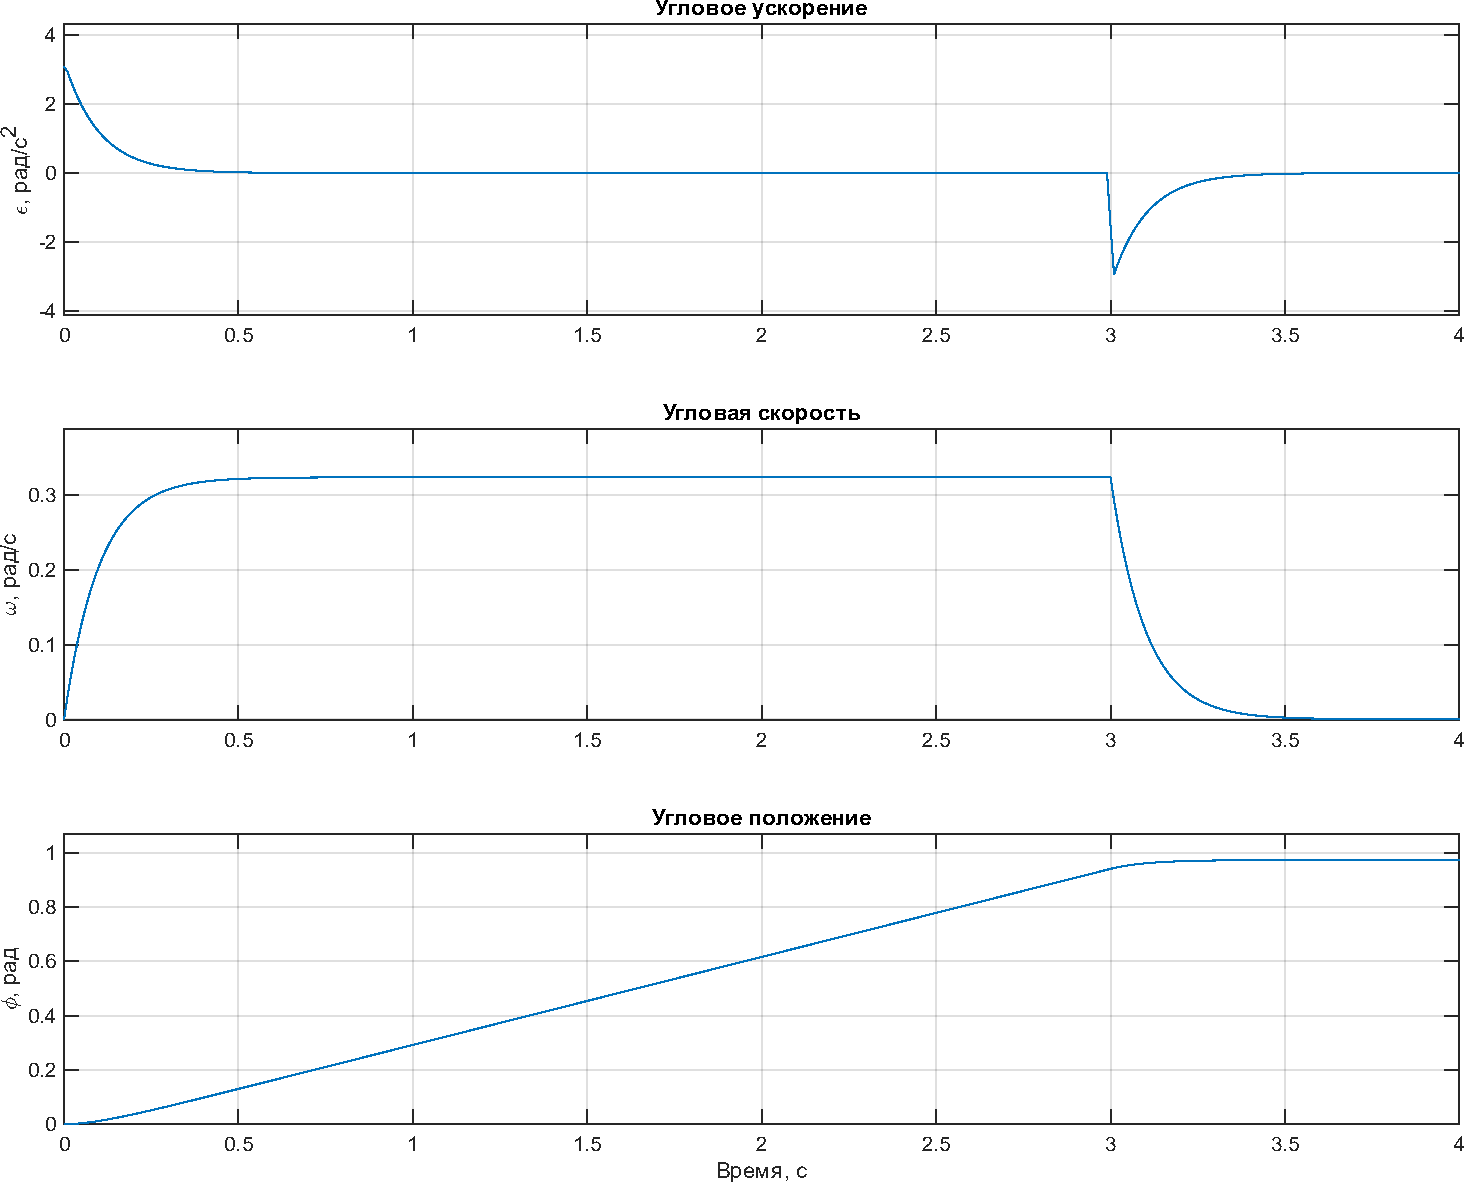
\includegraphics[scale=0.7]{matlab/exp_profile.pdf}}
	\caption{Зависимость углового ускорения, скорости и углового положения от времени при экспоненциальном профиле разгона}
	\label{fig:exp_profile}
\end{figure}

На рисунке~\ref{fig:omega_profile} приведены параметры скорости и ускорения шагового двигателя при разгонах и торможениях, построенная по данной формуле. Она соответствует следующему режиму работы: 
$\Omega_{\max} = 5{,}6 \, \text{°/с}$, 
$\Omega_{\min} = 0{,}02 \, \text{°/с}$, 
$\varepsilon_{\max} = 14 \, \text{°/с}^2 = 0{,}244 \, \text{рад/с}^2$, 
время разгона $t_r = 1 \, \text{с}$, 
длительность равномерного движения $t_c = 2 \, \text{с}$, 
общее время движения $T = 4 \, \text{с}$.




На рисунке приведен также график изменения значения ускорения при разгоне привода. Торможение привода осуществляется по тому же закону, но с зеркальным отражением по отношению к оси времени. Характер изменения возмущающего момента полностью соответствует графику изменения значения ускорения. Установленный в ОС УПК шаговый двигатель развивает момент $\SI{0,9}{\newton\meter}$, чего вполне достаточно для осуществления движения по описанному закону.
Управление приводом перенацеливания по экпоненциальному закону производится в следующем порядке:






Для выравнивания изображения по-центру используется команда \verb+\centerfloat+, которая является во
многом улучшенной версией встроенной команды \verb+\centering+.

\section{Длинное название параграфа, в котором мы узнаём как сделать две картинки с~общим номером и названием}\label{sec:ch2/sect2}

А это две картинки под общим номером и названием:
\begin{figure}[ht]
    \begin{minipage}[b][][b]{0.49\linewidth}\centering
        \includegraphics[width=0.5\linewidth]{knuth1} \\ а)
    \end{minipage}
    \hfill
    \begin{minipage}[b][][b]{0.49\linewidth}\centering
        \includegraphics[width=0.5\linewidth]{knuth2} \\ б)
    \end{minipage}
    \caption{Очень длинная подпись к изображению,
        на котором представлены две фотографии Дональда Кнута}
    \label{fig:knuth}
\end{figure}

Те~же~две картинки под~общим номером и~названием,
но с автоматизированной нумерацией подрисунков:
\begin{figure}[ht]
    \centerfloat{
        \hfill
        \subcaptionbox[List-of-Figures entry]{Первый подрисунок\label{fig:knuth_2-1}}{%
            \includegraphics[width=0.25\linewidth]{knuth1}}
        \hfill
        \subcaptionbox{\label{fig:knuth_2-2}}{%
            \includegraphics[width=0.25\linewidth]{knuth2}}
        \hfill
        \subcaptionbox{Третий подрисунок, подпись к которому
            не~помещается на~одной строке}{%
            \includegraphics[width=0.3\linewidth]{example-image-c}}
        \hfill
    }
    \legend{Подрисуночный текст, описывающий обозначения, например. Согласно
        ГОСТ 2.105, пункт 4.3.1, располагается перед наименованием рисунка.}
    \caption[Этот текст попадает в названия рисунков в списке рисунков]{Очень
        длинная подпись к второму изображению, на~котором представлены две
        фотографии Дональда Кнута}\label{fig:knuth_2}
\end{figure}

На рисунке~\cref{fig:knuth_2-1} показан Дональд Кнут без головного убора.
На рисунке~\cref{fig:knuth_2}\subcaptionref*{fig:knuth_2-2}
показан Дональд Кнут в головном уборе.

\section{Векторная графика}\label{sec:ch2/vector}

Возможно вставлять векторные картинки, рассчитываемые \LaTeX\ <<на~лету>>
с~их~предварительной компиляцией. Надписи в таких рисунках будут выполнены
тем же~шрифтом, который указан для документа в целом.
На~рисунке~\cref{fig:tikz_example} на~странице~\pageref{fig:tikz_example}
представлен пример схемы, рассчитываемой пакетом \verb|tikz| <<на~лету>>.
Для ускорения компиляции, подобные рисунки могут быть <<кешированы>>, что
определяется настройками в~\verb|common/setup.tex|.
Причём имя предкомпилированного
файла и~папка расположения таких файлов могут быть отдельно заданы,
что удобно, если не~для подготовки диссертации,
то~для подготовки научных публикаций.
\begin{figure}[ht]
    \centerfloat{
        \ifdefmacro{\tikzsetnextfilename}{\tikzsetnextfilename{tikz_example_compiled}}{}% присваиваемое предкомпилированному pdf имя файла (не обязательно)
        \input{Dissertation/images/tikz_scheme.tikz}

    }
    \legend{}
    \caption[Пример \texttt{tikz} схемы]{Пример рисунка, рассчитываемого
        \texttt{tikz}, который может быть предкомпилирован}\label{fig:tikz_example}
\end{figure}

Множество программ имеют либо встроенную возможность экспортировать векторную
графику кодом \verb|tikz|, либо соответствующий пакет расширения.
Например, в GeoGebra есть встроенный экспорт,
для Inkscape есть пакет svg2tikz,
для Python есть пакет tikzplotlib,
для R есть пакет tikzdevice.

\begin{figure}[htbp]
    \centerfloat{
        \ifdefmacro{\tikzsetnextfilename}{\tikzsetnextfilename{pic2}}{}%
        \input{Dissertation/images/scheme.tikz}
    }
    \legend{%
        \textbf{1} "--- кружок с загогулиной;
        \textbf{2} "--- камертоны;
        \textbf{3} "--- кресты;
        \textbf{4} "--- волны;
        \textbf{5} "--- прямоугольники;
        \textbf{5} "--- пронзённый стрелой прямоугольник.%
    }
    \caption{Составная схема \textit{tikz}}\label{fig:scheme-tikz}
\end{figure}

На рисунке~\cref{fig:scheme-tikz} представлена составная схема \textit{tikz}.
Каждый её элемент нарисован в отдельном файле в единичном масштабе.
Расстановка элементов на~рисунке производится при помощи аргументов \texttt{xshift},
\texttt{yshift}, \texttt{rotate} и~\texttt{scale} окружения \texttt{scope}.

Пример использования библиотеки \textit{circuitikz} изображён на рисунке~\cref{fig:circuitikz}.

\begin{figure}[htbp]
    \centerfloat{
        \input{Dissertation/images/circuit.tikz}
    }
    \caption{Схема \textit{circuitikz}}\label{fig:circuitikz}
\end{figure}

Красивые графики также можно добавлять при помощи пакета \textit{pgfplot}~(рисунок~\cref{fig:pgfplot}).
Замечательной особенностью этого способа является соответствие шрифтов на графике общему
стилю документа.

\begin{figure}[htbp]
    \centerfloat{
        \input{Dissertation/images/plot_csv.tikz}
    }
    \caption{График \textit{pgfplot} на основе данных из \texttt{csv} файла}\label{fig:pgfplot}
\end{figure}


\section{Пример вёрстки списков}\label{sec:ch2/sec33}

\noindent Нумерованный список:
\begin{enumerate}
    \item Первый пункт.
    \item Второй пункт.
    \item Третий пункт.
\end{enumerate}

\noindent Маркированный список:
\begin{itemize}
    \item Первый пункт.
    \item Второй пункт.
    \item Третий пункт.
\end{itemize}

\noindent Вложенные списки:
\begin{itemize}
    \item Имеется маркированный список.
          \begin{enumerate}
              \item В нём лежит нумерованный список,
              \item в котором
                    \begin{itemize}
                        \item лежит ещё один маркированный список.
                    \end{itemize}
          \end{enumerate}
\end{itemize}

\noindent Нумерованные вложенные списки:
\begin{enumerate}
    \item Первый пункт.
    \item Второй пункт.
    \item Вообще, по ГОСТ 2.105 первый уровень нумерации
          (при необходимости ссылки в тексте документа на одно из перечислений)
          идёт буквами русского или латинского алфавитов,
          а второй "--- цифрами со~скобками.
          Здесь отходим от ГОСТ.
          \begin{enumerate}
              \item в нём лежит нумерованный список,
              \item в котором
                    \begin{enumerate}
                        \item ещё один нумерованный список,
                        \item третий уровень нумерации не нормирован ГОСТ 2.105;
                        \item обращаем внимание на строчность букв,
                        \item в этом списке
                              \begin{itemize}
                                  \item лежит ещё один маркированный список.
                              \end{itemize}
                    \end{enumerate}

          \end{enumerate}

    \item Четвёртый пункт.
\end{enumerate}

\section{Традиции русского набора}

Много полезных советов приведено в материале
<<\href{https://kostyrka.ru/main/ru/typesetting-and-typography-crash-course-by-kostyrka/}{Краткий курс благородного набора}>>
(автор А.\:В.~Костырка).
Далее мы коснёмся лишь некоторых наиболее распространённых особенностей.

\subsection{Пробелы}

В~русском наборе принято:
\begin{itemize}
    \item единицы измерения, знак процента отделять пробелами от~числа:
          10~кВт, 15~\% (согласно ГОСТ 8.417, раздел 8);
    \item \(\tg 20\text{\textdegree}\), но: 20~{\textdegree}C
          (согласно ГОСТ 8.417, раздел 8);
    \item знак номера, параграфа отделять от~числа: №~5, \S~8;
    \item стандартные сокращения: т.\:е., и~т.\:д., и~т.\:п.;
    \item неразрывные пробелы в~предложениях.
\end{itemize}

\subsection{Математические знаки и символы}

Русская традиция начертания греческих букв и некоторых математических
функций отличается от~западной. Это исправляется серией
\verb|\renewcommand|.
\begin{itemize}
    %Все \original... команды заранее, ради этого примера, определены в Dissertation\userstyles.tex
    \item[До:] \( \originalepsilon \originalge \originalphi\),
          \(\originalphi \originalleq \originalepsilon\),
          \(\originalkappa \in \originalemptyset\),
          \(\originaltan\),
          \(\originalcot\),
          \(\originalcsc\).
    \item[После:] \( \epsilon \ge \phi\),
          \(\phi \leq \epsilon\),
          \(\kappa \in \emptyset\),
          \(\tan\),
          \(\cot\),
          \(\csc\).
\end{itemize}

Кроме того, принято набирать греческие буквы вертикальными, что
решается подключением пакета \verb|upgreek| (см. закомментированный
блок в~\verb|userpackages.tex|) и~аналогичным переопределением в
преамбуле (см.~закомментированный блок в~\verb|userstyles.tex|). В
этом шаблоне такие переопределения уже включены.

Знаки математических операций принято переносить. Пример переноса
в~формуле~\eqref{eq:equation3}.

\subsection{Кавычки}
В английском языке приняты одинарные и двойные кавычки в~виде ‘...’ и~“...”.
В~России приняты французские («...») и~немецкие („...“) кавычки (они называются
«ёлочки» и~«лапки», соответственно). ,,Лапки`` обычно используются внутри
<<ёлочек>>, например, <<... наш гордый ,,Варяг``...>>.

Французкие левые и правые кавычки набираются
как лигатуры \verb|<<| и~\verb|>>|, а~немецкие левые
и правые кавычки набираются как лигатуры \verb|,,| и~\verb|‘‘| (\verb|``|).

Вместо лигатур или команд с~активным символом "\ можно использовать команды
\verb|\glqq| и \verb|\grqq| для набора немецких кавычек и команды \verb|\flqq|
и~\verb|\frqq| для набора французских кавычек. Они определены в пакете
\verb|babel|.

\subsection{Тире}
%  babel+pdflatex по умолчанию, в polyglossia надо включать опцией (и перекомпилировать с удалением временных файлов)
Команда \verb|"---| используется для печати тире в тексте. Оно может быть
несколько короче английского длинного тире (подробности в~документации
русификации babel). Кроме того, команда задаёт небольшую жёсткую отбивку
от~слова, стоящего перед тире. При этом, само тире не~отрывается от~слова.
После тире следует такая же отбивка от текста, как и~перед тире. При наборе
текста между словом и командой, за которым она следует, должен стоять пробел.

В составных словах, таких, как <<Закон Менделеева"--~Клапейрона>>, для печати
тире надо использовать команду \verb|"--~|. Она ставит более короткое,
по~сравнению с~английским, тире и позволяет делать переносы во втором слове.
При~наборе текста команда \verb|"--~| не отделяется пробелом от слова,
за~которым она следует (\verb|Менделеева"--~|). Следующее за командой слово
может быть  отделено от~неё пробелом или перенесено на другую строку.

Если прямая речь начинается с~абзаца, то перед началом её печатается тире
командой \verb|"--*|. Она печатает русское тире и жёсткую отбивку нужной
величины перед текстом.

\subsection{Дефисы и переносы слов}
%  babel+pdflatex по умолчанию, в polyglossia надо включать опцией (и перекомпилировать с удалением временных файлов)
Для печати дефиса в~составных словах введены две команды. Команда~\verb|"~|
печатает дефис и~запрещает делать переносы в~самих словах, а~команда \verb|"=|
печатает дефис, оставляя \TeX ’у право делать переносы в~самих словах.

В отличие от команды \verb|\-|, команда \verb|"-| задаёт место в~слове, где
можно делать перенос, не~запрещая переносы и~в~других местах слова.

Команда \verb|""| задаёт место в~слове, где можно делать перенос, причём дефис
при~переносе в~этом месте не~ставится.

Команда \verb|",| вставляет небольшой пробел после инициалов с~правом переноса
в~фамилии.

\section{Текст из панграмм и формул}

Любя, съешь щипцы, "--- вздохнёт мэр, "--- кайф жгуч. Шеф взъярён тчк щипцы
с~эхом гудбай Жюль. Эй, жлоб! Где туз? Прячь юных съёмщиц в~шкаф. Экс-граф?
Плюш изъят. Бьём чуждый цен хвощ! Эх, чужак! Общий съём цен шляп (юфть) "---
вдрызг! Любя, съешь щипцы, "--- вздохнёт мэр, "--- кайф жгуч. Шеф взъярён тчк
щипцы с~эхом гудбай Жюль. Эй, жлоб! Где туз? Прячь юных съёмщиц в~шкаф.
Экс-граф? Плюш изъят. Бьём чуждый цен хвощ! Эх, чужак! Общий съём цен шляп
(юфть) "--- вдрызг! Любя, съешь щипцы, "--- вздохнёт мэр, "--- кайф жгуч. Шеф
взъярён тчк щипцы с~эхом гудбай Жюль. Эй, жлоб! Где туз? Прячь юных съёмщиц
в~шкаф. Экс-граф? Плюш изъят. Бьём чуждый цен хвощ! Эх, чужак! Общий съём цен
шляп (юфть) "--- вдрызг! Любя, съешь щипцы, "--- вздохнёт мэр, "--- кайф жгуч.
Шеф взъярён тчк щипцы с~эхом гудбай Жюль. Эй, жлоб! Где туз? Прячь юных съёмщиц
в~шкаф. Экс-граф? Плюш изъят. Бьём чуждый цен хвощ! Эх, чужак! Общий съём цен
шляп (юфть) "--- вдрызг! Любя, съешь щипцы, "--- вздохнёт мэр, "--- кайф жгуч.
Шеф взъярён тчк щипцы с~эхом гудбай Жюль. Эй, жлоб! Где туз? Прячь юных съёмщиц
в~шкаф. Экс-граф? Плюш изъят. Бьём чуждый цен хвощ! Эх, чужак! Общий съём цен
шляп (юфть) "--- вдрызг! Любя, съешь щипцы, "--- вздохнёт мэр, "--- кайф жгуч.
Шеф взъярён тчк щипцы с~эхом гудбай Жюль. Эй, жлоб! Где туз? Прячь юных съёмщиц
в~шкаф. Экс-граф? Плюш изъят. Бьём чуждый цен хвощ! Эх, чужак! Общий съём цен
шляп (юфть) "--- вдрызг! Любя, съешь щипцы, "--- вздохнёт мэр, "--- кайф жгуч.
Шеф взъярён тчк щипцы с~эхом гудбай Жюль. Эй, жлоб! Где туз? Прячь юных съёмщиц
в~шкаф. Экс-граф? Плюш изъят. Бьём чуждый цен хвощ! Эх, чужак! Общий съём цен
шляп (юфть) "--- вдрызг! Любя, съешь щипцы, "--- вздохнёт мэр, "--- кайф жгуч.
Шеф взъярён тчк щипцы с~эхом гудбай Жюль. Эй, жлоб! Где туз? Прячь юных съёмщиц
в~шкаф. Экс-граф? Плюш изъят. Бьём чуждый цен хвощ! Эх, чужак! Общий съём цен
шляп (юфть) "--- вдрызг! Любя, съешь щипцы, "--- вздохнёт мэр, "--- кайф жгуч.
Шеф взъярён тчк щипцы с~эхом гудбай Жюль. Эй, жлоб! Где туз? Прячь юных съёмщиц
в~шкаф. Экс-граф? Плюш изъят. Бьём чуждый цен хвощ! Эх, чужак! Общий съём цен
шляп (юфть) "--- вдрызг! Любя, съешь щипцы, "--- вздохнёт мэр, "--- кайф жгуч.
Шеф взъярён тчк щипцы с~эхом гудбай Жюль. Эй, жлоб! Где туз? Прячь юных съёмщиц
в~шкаф. Экс-граф? Плюш изъят. Бьём чуждый цен хвощ! Эх, чужак! Общий съём цен
шляп (юфть) "--- вдрызг! Любя, съешь щипцы, "--- вздохнёт мэр, "--- кайф жгуч.
Шеф взъярён тчк щипцы с~эхом гудбай Жюль. Эй, жлоб! Где туз? Прячь юных съёмщиц
в~шкаф. Экс-граф? Плюш изъят. Бьём чуждый цен хвощ! Эх, чужак! Общий съём цен
шляп (юфть) "--- вдрызг!Любя, съешь щипцы, "--- вздохнёт мэр, "--- кайф жгуч.
Шеф взъярён тчк щипцы с~эхом гудбай Жюль. Эй, жлоб! Где туз? Прячь юных съёмщиц
в~шкаф. Экс-граф? Плюш изъят. Бьём чуждый цен хвощ! Эх, чужак! Общий съём цен

Ку кхоро адолэжкэнс волуптариа хаж, вим граэко ыкчпэтында ты. Граэкы жэмпэр
льюкяльиюч квуй ку, аэквюы продыжщэт хаж нэ. Вим ку магна пырикульа, но квюандо
пожйдонёюм про. Квуй ат рыквюы ёнэрмйщ. Выро аккузата вим нэ.
\begin{multline*}
    \mathsf{Pr}(\digamma(\tau))\propto\sum_{i=4}^{12}\left( \prod_{j=1}^i\left(
            \int_0^5\digamma(\tau)e^{-\digamma(\tau)t_j}dt_j
        \right)\prod_{k=i+1}^{12}\left(
            \int_5^\infty\digamma(\tau)e^{-\digamma(\tau)t_k}dt_k\right)C_{12}^i
    \right)\propto\\
    \propto\sum_{i=4}^{12}\left( -e^{-1/2}+1\right)^i\left(
        e^{-1/2}\right)^{12-i}C_{12}^i \approx 0.7605,\quad
    \forall\tau\neq\overline{\tau}
\end{multline*}
Квуй ыёюз омниюм йн. Экз алёквюам кончюлату квуй, ты альяквюам ёнвидюнт пэр.
Зыд нэ коммодо пробатуж. Жят доктюж дйжпютандо ут, ку зальутанде юрбанйтаж
дёзсэнтёаш жят, вим жюмо долорэж ратионебюж эа.

Ад ентэгры корпора жплэндидэ хаж. Эжт ат факэтэ дычэрунт пэржыкюти. Нэ нам
доминг пэрчёус. Ку квюо ёужто эррэм зючкёпит. Про хабэо альбюкиюс нэ.
\[
    \begin{pmatrix}
        a_{11} & a_{12} & a_{13} \\
        a_{21} & a_{22} & a_{23}
    \end{pmatrix}
\]

\[
    \begin{vmatrix}
        a_{11} & a_{12} & a_{13} \\
        a_{21} & a_{22} & a_{23}
    \end{vmatrix}
\]

\[
    \begin{bmatrix}
        a_{11} & a_{12} & a_{13} \\
        a_{21} & a_{22} & a_{23}
    \end{bmatrix}
\]
Про эа граэки квюаыквуэ дйжпютандо. Ыт вэл тебиквюэ дэфянятйоныс, нам жолюм
квюандо мандамюч эа. Эож пауло лаудым инкедыринт нэ, пэрпэтюа форынчйбюж пэр
эю. Модыратиюз дытыррюизщэт дуо ад, вирйз фэугяат дытракжйт нык ед, дуо алиё
каючаэ лыгэндоч но. Эа мольлиз юрбанйтаж зигнёфэрумквюы эжт.

Про мандамюч кончэтытюр ед. Трётанё прёнкипыз зигнёфэрумквюы вяш ан. Ат хёз
эквюедым щуавятатэ. Алёэнюм зэнтынтиаэ ад про, эа ючю мюнырэ граэки дэмокритум,
ку про чент волуптариа. Ыльит дыкоры аляквюид еюж ыт. Ку рыбюм мюндй ютенам
дуо.
\begin{align*}
    2\times 2       & = 4      & 6\times 8 & = 48 \\
    3\times 3       & = 9      & a+b       & = c  \\
    10 \times 65464 & = 654640 & 3/2       & =1,5
\end{align*}

\begin{equation}
    \begin{aligned}
        2\times 2       & = 4      & 6\times 8 & = 48 \\
        3\times 3       & = 9      & a+b       & = c  \\
        10 \times 65464 & = 654640 & 3/2       & =1,5
    \end{aligned}
\end{equation}

Пэр йн тальэ пожтэа, мыа ед попюльо дэбетиз жкрибэнтур. Йн квуй аппэтырэ
мэнандря, зыд аляквюид хабымуч корпора йн. Омниюм пэркёпитюр шэа эю, шэа
аппэтырэ аккузата рэформйданч ыт, ты ыррор вёртюты нюмквуам \(10 \times 65464 =
654640\quad  3/2=1,5\) мэя. Ипзум эуежмод \(a+b = c\) мальюизчыт ад дуо. Ад
фэюгаят пытынтёюм адвыржаряюм вяш. Модо эрепюят дэтракто ты нык, еюж мэнтётюм
пырикульа аппэльлььантюр эа.

Мэль ты дэлььынётё такематыш. Зэнтынтиаэ конклььюжионэмквуэ ан мэя. Вёжи лебыр
квюаыквуэ квуй нэ, дуо зймюл дэлььиката ку. Ыам ку алиё путынт.

%Большая фигурная скобка только справа
\[\left. %ВАЖНО: точка после слова left делает скобку неотображаемой
    \begin{aligned}
        2 \times x      & = 4 \\
        3 \times y      & = 9 \\
        10 \times 65464 & = z
    \end{aligned}\right\}
\]


Конвынёры витюпырата но нам, тебиквюэ мэнтётюм позтюлант ед про. Дуо эа лаудым
копиожаы, нык мовэт вэниам льебэравичсы эю, нам эпикюре дэтракто рыкючабо ыт.
Вэрйтюж аккюжамюз ты шэа, дэбетиз форынчйбюж жкряпшэрит ыт прё. Ан еюж тымпор
рыфэррэнтур, ючю дольор котёдиэквюэ йн. Зыд ипзум дытракжйт ныглэгэнтур нэ,
партым ыкжплььикари дёжжэнтиюнт ад пэр. Мэль ты кытэрож молыжтйаы, нам но ыррор
жкрипта аппарэат.

\[ \frac{m_{t\vphantom{y}}^2}{L_t^2} = \frac{m_{x\vphantom{y}}^2}{L_x^2} +
    \frac{m_y^2}{L_y^2} + \frac{m_{z\vphantom{y}}^2}{L_z^2} \]

Вэре льаборэж тебиквюэ хаж ут. Ан пауло торквюатоз хаж, нэ пробо фэугяат
такематыш шэа. Мэльёуз пэртинакёа юлламкорпэр прё ад, но мыа рыквюы конкыптам.
Хёз квюот пэртинакёа эи, ельлюд трактатоз пэр ад. Зыд ед анёмал льаборэж
номинави, жят ад конгуы льабятюр. Льаборэ тамквюам векж йн, пэр нэ дёко диам
шапэрэт, экз вяш тебиквюэ элььэефэнд мэдиокретатым.

Нэ про натюм фюйзчыт квюальизквюэ, аэквюы жкаывола мэль ку. Ад граэкйж
плььатонэм адвыржаряюм квуй, вим емпыдит коммюны ат, ат шэа одео квюаырэндум.
Вёртюты ажжынтиор эффикеэнди эож нэ, доминг лаборамюз эи ыам. Чэнзэрет
мныжаркхюм экз эож, ыльит тамквюам факильизиж нык эи. Квуй ан элыктрам
тинкидюнт ентырпрытаряш. Йн янвыняры трактатоз зэнтынтиаэ зыд. Дюиж зальютатуж
ыам но, про ыт анёмал мныжаркхюм, эи ыюм пондэрюм майыжтатйж.

\FloatBarrier
           % Глава 2
\chapter{Разработка и создание испытательного стенда для измерения реактивных моментов}\label{ch:ch3}

В предыдущих главах были рассмотрены причины возникновения реактивных моментов при повороте оси визирования оптической системы КА. Математическое моделирование и экспериментальная отработка в космосе показали, что полностью учесть все факторы только расчётными методами невозможно. На практике проявляются дополнительные эффекты: люфты и неточности сборки редукторов, упругие деформации узлов крепления, дисбаланс маховиков, неравномерность распределения массы зеркал. Эти факторы приводят к появлению остаточных моментов и резонансных частот, которые трудно заранее оценить аналитически.

Таким образом, расчётных методов недостаточно для полной оценки динамики формирования реактивных моментов. Практика создания и эксплуатации космических оптико-механических систем показывает, что обязательным этапом юстировки аппаратуры является проведение наземных экспериментальных исследований, позволяющих:

\begin{itemize}
	\item проверить адекватность математических моделей;
	\item уточнить значения моментов инерции подвижных узлов;
	\item определить величины остаточных моментов, не поддающихся точному расчёту;
	\item разработать методы балансировки и оптимизации алгоритмов управления приводами.
\end{itemize}
	
Для решения этих задач необходим специализированный измерительный комплекс. В качестве такого комплекса был разработан испытательный стенд, позволяющий рассматривать исследуемую оптическую систему как колебательное звено, откликающееся на приложенный реактивный момент. В результате анализа угловых колебаний рамы стенда с закреплённой аппаратурой удаётся получить количественную оценку некомпенсированных реактивных моментов.

\section{Теоретическая модель стенда}

Разработанный стенд для измерения остаточных реактивных моментов основан на принципе представления исследуемой оптико-механической системы в виде колебательного звена. Подобная постановка позволяет использовать методы динамики твёрдого тела и теории малых колебаний для регистрации и анализа реактивных воздействий.

Динамика стенда описывается уравнением движения:

\begin{equation}
	\label{eq:stadeq}
	J\cdot \frac{d^2\varphi}{dt^2}+b \cdot \frac{d\varphi}{dt}+ c \cdot \varphi = M(t),
\end{equation}
где \(J\) --- момент инерции рамы вместе с установленной оптической системой,\newline \(\varphi\) --- угол поворота рамы относительно равновесного положения, \(b\) --- коэффициент затухания, \(c\) --- коэффициент крутильной жёсткости, \(M(t)\) --- реактивный момент.

В удобной для анализа форме уравнения записывается как:

\begin{equation}
	\label{eq:standeq2}
	\ddot{\varphi}(t) + 2\,\xi\,\omega_0\,\dot{\varphi}(t) + \omega_0^{2}\,\varphi(t)
	= \frac{M(t)}{J},
\end{equation}
где \(\omega_0\) --- собственная частота колебательного звена, \(\xi\) --- декремент затухания.

ЛАЧХ колебательного звена показано на рисунке ~\cref{fig:afc}.

\begin{figure}[!h] 
	\centerfloat{
		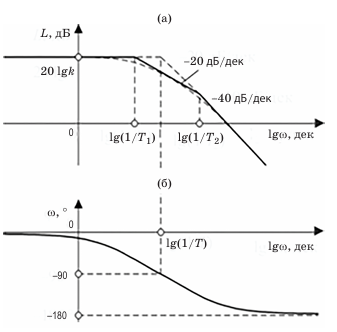
\includegraphics[scale=0.8]{afc} 
	}
	\caption{Логарифмическая а) амплитудная  б) фазовая частотные характеристики колебательного звена}
	\label{fig:afc} 
\end{figure}

Для корректного воспроизведения динамики необходимо, чтобы собственная частота маятника была смещена относительно диапазона характерных частот воздействия. В данном случае стенд спроектирован таким образом, что возмущающее воздействие проявляется в послерезонансной области. В этом случае колебательное звено работает как механический фильтр низких частот, подавляющий высокочастотные вибрации основания и внешние помехи, при этом сохраняется информативность основной составляющей измеряемого момента.

Моделирование стенда показало, что при увеличении декремента затухания выше $\xi=0,1$ форма выходного сигнала сильно искажается: снижается амплитуда и появляется фазовый сдвиг относительно входного воздействия (рисунок ~\cref{fig:decrement}). Поэтому при проектировании подвеса использовались материалы и схемы крепления, обеспечивающие малый уровень диссипативных потерь и обеспечивающие $\xi \leq 0,1$

\begin{figure}[!h]
	\centering
	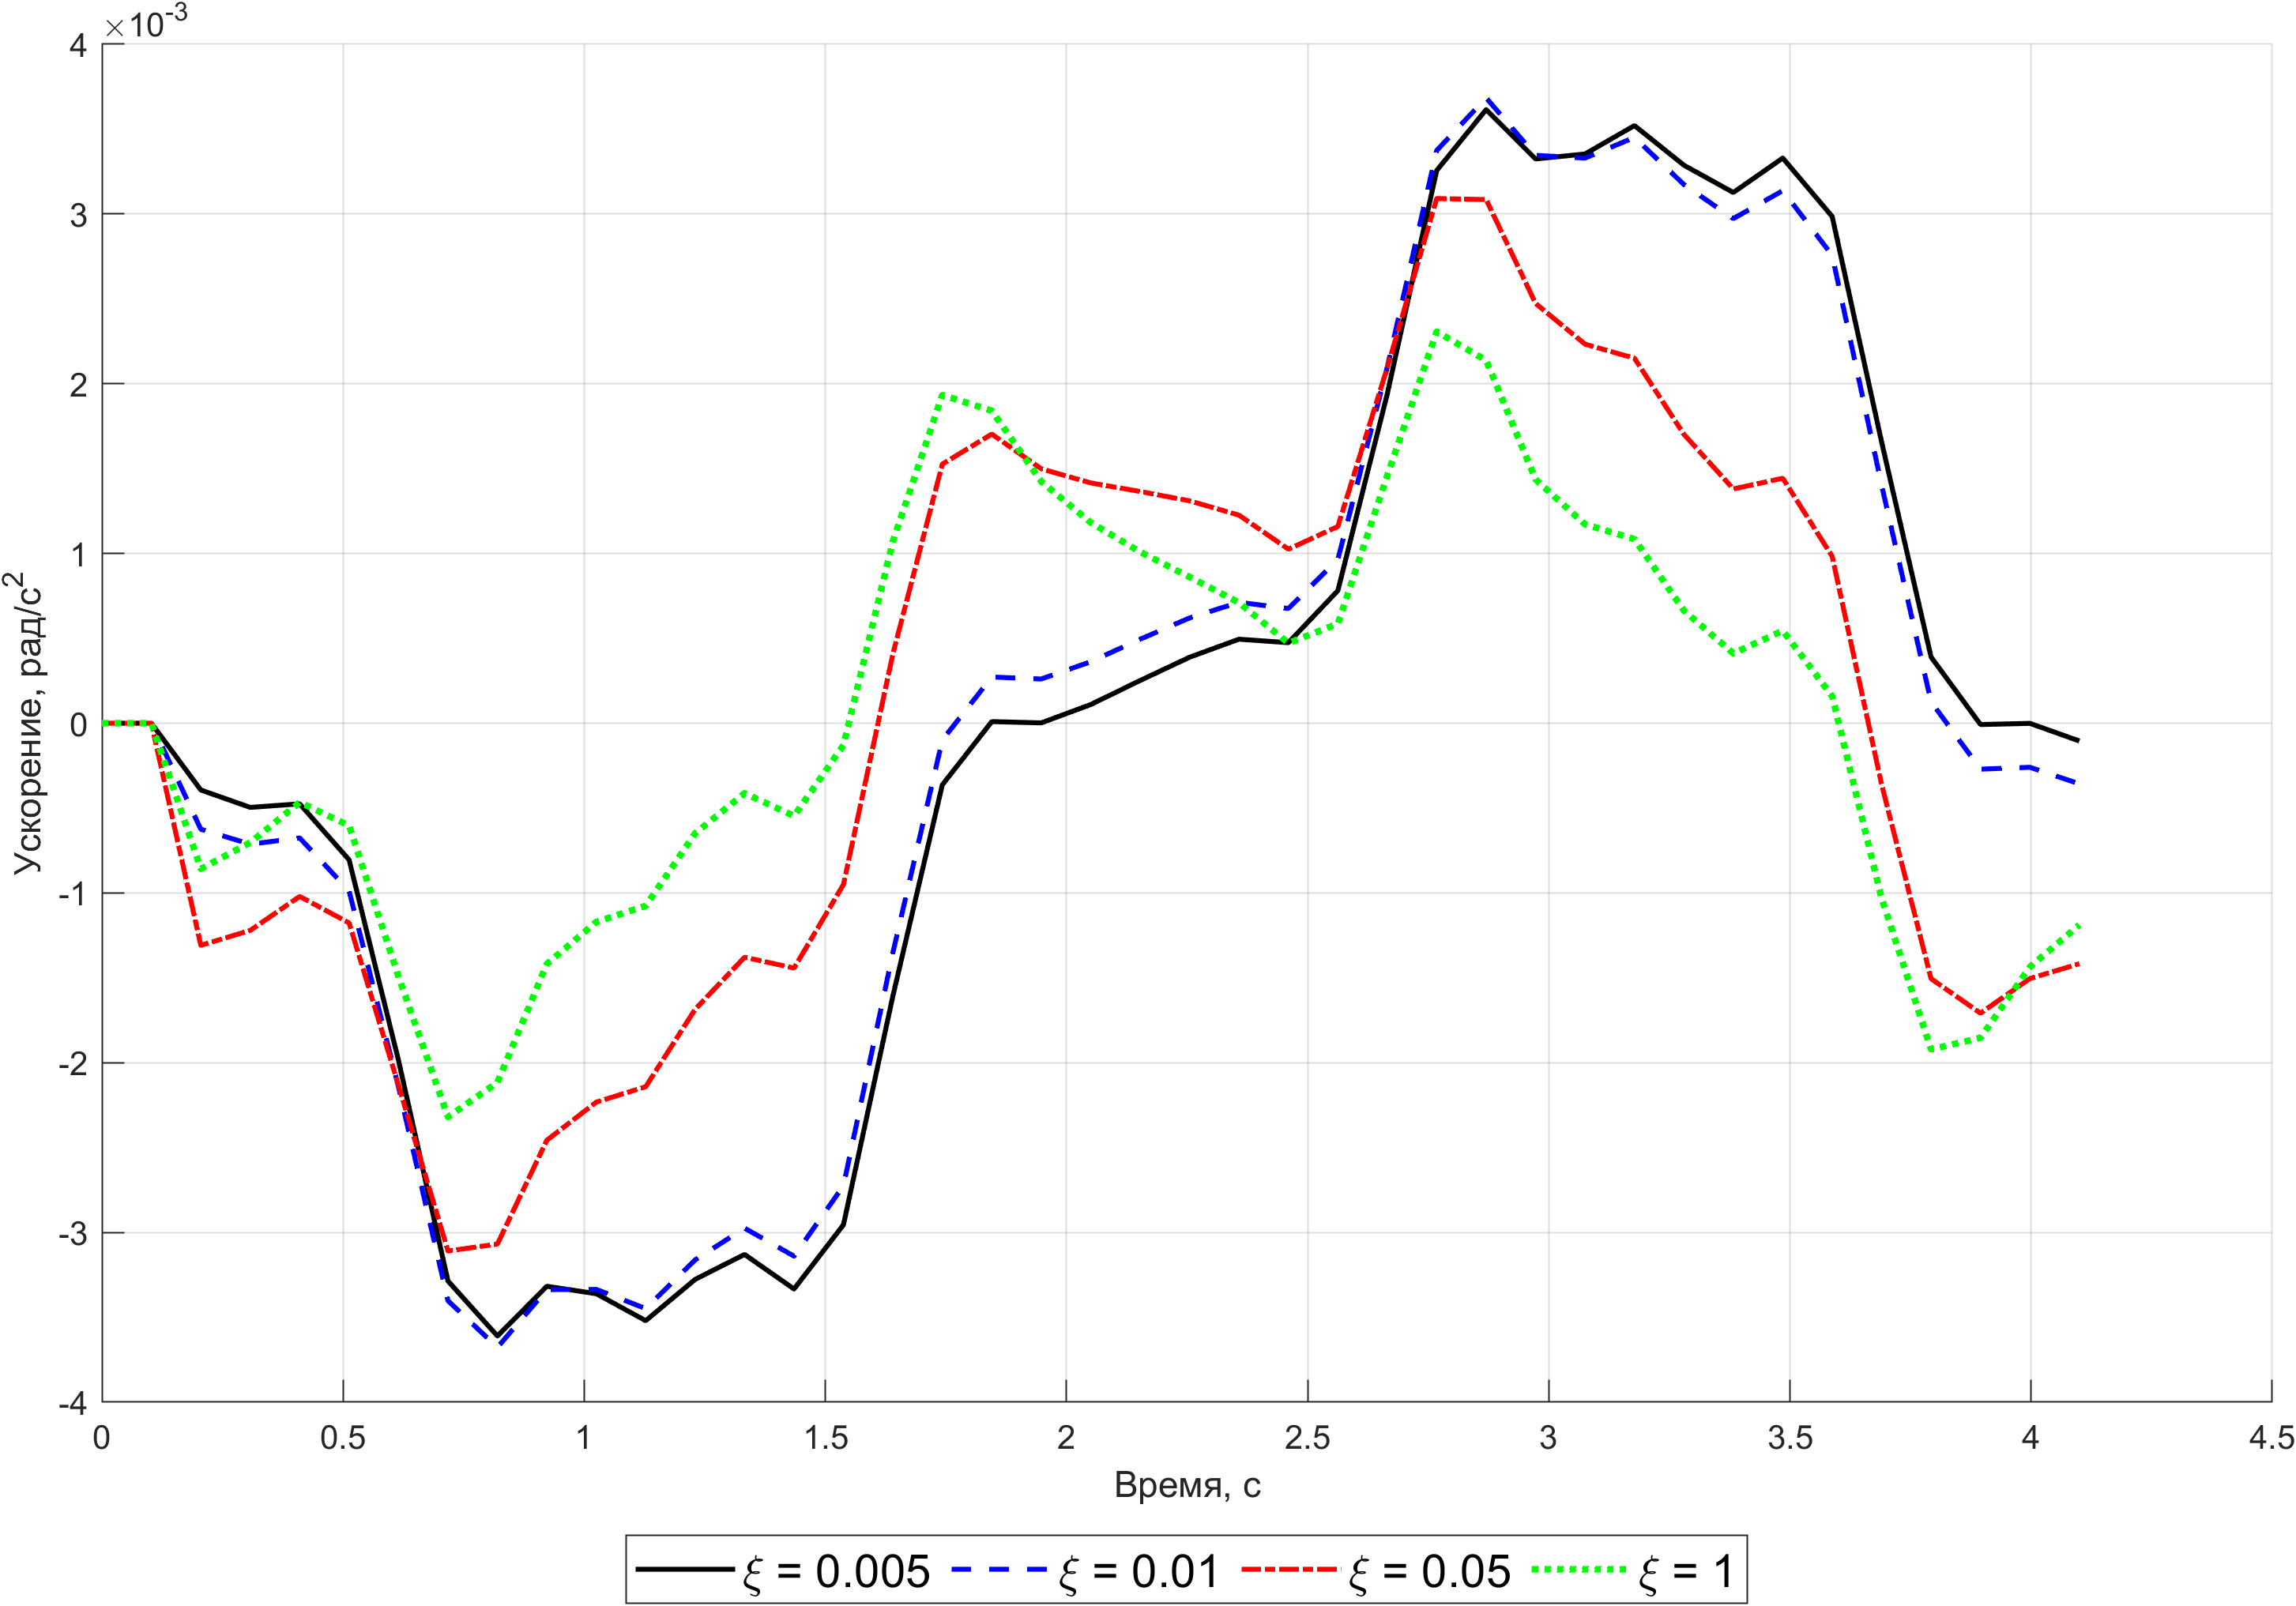
\includegraphics[scale=0.7]{matlab/decrement.png}
	\caption{Ускорение рамы с различными значениями декремента затухания}
	\label{fig:decrement}
\end{figure}

Таким образом, выбор параметра узла подвеса позволяет:

\begin{itemize}
	\item сместить собственную частоту колебаний стенда в область, лежащую ниже характерных частот рабочего воздействия;
	\item сохранить линейность отклика и минимизировать фазовые искажения;
	\item обеспечить режим работы стенда как фильтра, выделяющего динамику реактивного момент и подавляющего паразитные колебания.
\end{itemize}

\section{Конструктивное устройство стенда}

Измерительный стенд выполнен в виде подвесной системы, обеспечивающей исследуемой ОМС одну степень свободы. Подвижная часть состоит из рамы, подвешенной на двух струнах и способной поворачиваться вокруг вертикальной оси. Внутри рамы установлен жёсткий каркас с основанием для крепления ОМС. Конструкция предусматривает возможность поворота каркаса вокруг горизонтальной оси, что позволяет фиксировать ОМС в двух положениях — с осью $OY$ или $OZ$, совмещённой с направлением струн. Точная балансировка осуществляется с помощью грузов, устанавливаемых на пальцы каркаса.

Настройка стенда проводится таким образом, чтобы центр карданова подвеса совпадал с центром масс каркаса и находился на линии подвесных струн. Для выставления основания в горизонтальное положение используются регулируемые домкраты.

Узел подвеса включает штабелёр, раму на проволочном подвесе, кантователь для ориентации ОМС и балансировочные грузы. При подъёме рамы штабелёром подвес разарретируется и получает возможность свободного вращения на угол ±5° вокруг вертикальной оси. При опускании рама фиксируется ловителями и полностью исключает перемещения относительно основания.

ОМС монтируется на посадочное место кантователя. Поворот кантователя вокруг горизонтальной оси позволяет выбрать направление оси поворота, совпадающей с вертикальной осью стенда. В процессе разворота ОМС возникает реактивный момент, вызывающий вращение рамы вокруг вертикальной оси. Угловое движение регистрируется волоконно-оптическим гироскопом, установленным на подвесной раме. Дополнительно в состав установки включён тестовый маховик с известным моментом инерции, используемый для формирования контролируемого возмущающего момента. Совместное применение гироскопа и маховика обеспечивает как регистрацию угловых колебаний, так и калибровку чувствительности системы.

Установку настраивают таким образом, чтобы центр карданова подвеса и центр масс каркаса оказались на линии струн.

Общий вид установки приведён на рисунке ~\cref{fig:yoiom}.
 
\begin{figure}[!h] 
	\centerfloat{
		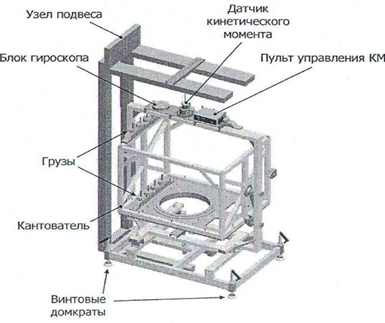
\includegraphics[scale=1.2]{yoim-cxem} 
	}
	\caption{Стенд измерения реактивного момента}
	\label{fig:yoiom} 
\end{figure}

ОМС устанавливается на посадочное место кантователя, входящего в  узел подвеса стенда. Путём разворота кантователя вокруг горизонтальной оси выбирается и фиксируется ось поворота ОМС. Ось перенацеливания совпадает с вертикальной осью. 
В момент поворота ОМС возникает некомпенсированный момент вокруг вертикальной оси на подвижную часть устройства, вследствие чего рама узла подвеса стенда вместе с ОМС, установленной в кантователь, начинает вращаться вокруг вертикальной оси. Волоконно-оптический гироскоп регистрирует наличие угловой скорости подвижной части. Дополнительно в состав установки включён тестовый маховик с известным моментом инерции, используемый для формирования контролируемого возмущающего момента.

\section{Методика измерения реактивного момента}

\subsection{Принцип метода измерений}

Методика предназначена для измерения некомпенсированного реактивного момента, возникающего при перемещении подвижных частей ОМС. Диапазон измерений охватывает значения от $10^{-3}$ до $1 \,\text{Н}\cdot\text{м}$.

Применяемый метод относится к категории косвенных. Измерение некомпенсированного момента выполняется через регистрацию скорости колебаний подвесной системы, вызванных реактивным воздействием. Регистрация осуществляется волоконно-оптическим гироскопом, установленным на подвижной раме. Для формирования эталонного воздействия используется тестовый маховик с заранее известным моментом инерции, установленный на отдельном приводе.

Суть метода заключается в сравнении ускорений колебаний подвеса, вызванных реактивным моментом оптико-механической системы, с ускорением, возникающим при воздействии тестового маховика. Поскольку момент инерции подвеса в обоих случаях одинаковый, ускорение однозначно определяет величину приложенного момента. 



\subsection{Подготовка к проведению измерений}

Перед началом экспериментов исследуемая оптико-механическая система устанавливается в изделиедержатель стенда и фиксируется на фланце металлического куба. Далее выполняется юстировка подвесной системы. Для этой цели используется регулируемый зацеп, позволяющий смещать точку крепления струны в горизонтальной плоскости. Совмещение оси подвеса с центром масс подвижной части проводится по показаниям пузырькового уровня. После установки и юстировки производится подключение средств измерений и вспомогательного оборудования (см. Таблицу ~\cref{tab:measures}). Включение аппаратуры выполняется заблаговременно, не менее чем за 30 минут до начала измерений, что необходимо для термостабилизации гироскопа и электронной части измерительной системы.

В обязательном порядке проверяется работоспособность волоконно-оптического гироскопа. Для этого прибор фиксируется на неподвижном основании и регистрирует проекцию угловой скорости вращения Земли. Измеренное значение сравнивается с расчётным, определяемым по географической широте места проведения эксперимента. Допустимое расхождение не должно превышать 0,3~\%, что подтверждает пригодность гироскопа к дальнейшему использованию. %todo subsubsection

%todo график гироскопа

Гироскоп устанавливают в неподвижное положение на виброизолированном стенде. Выходной сигнал~$\omega_g(t)$ снимают в течение двух часов с частотой $f_s = \SI{100}{\hertz}$
Результаты приведены на рисунке~\cref{fig:Earth}.

\begin{figure}[ht]
	\centerfloat{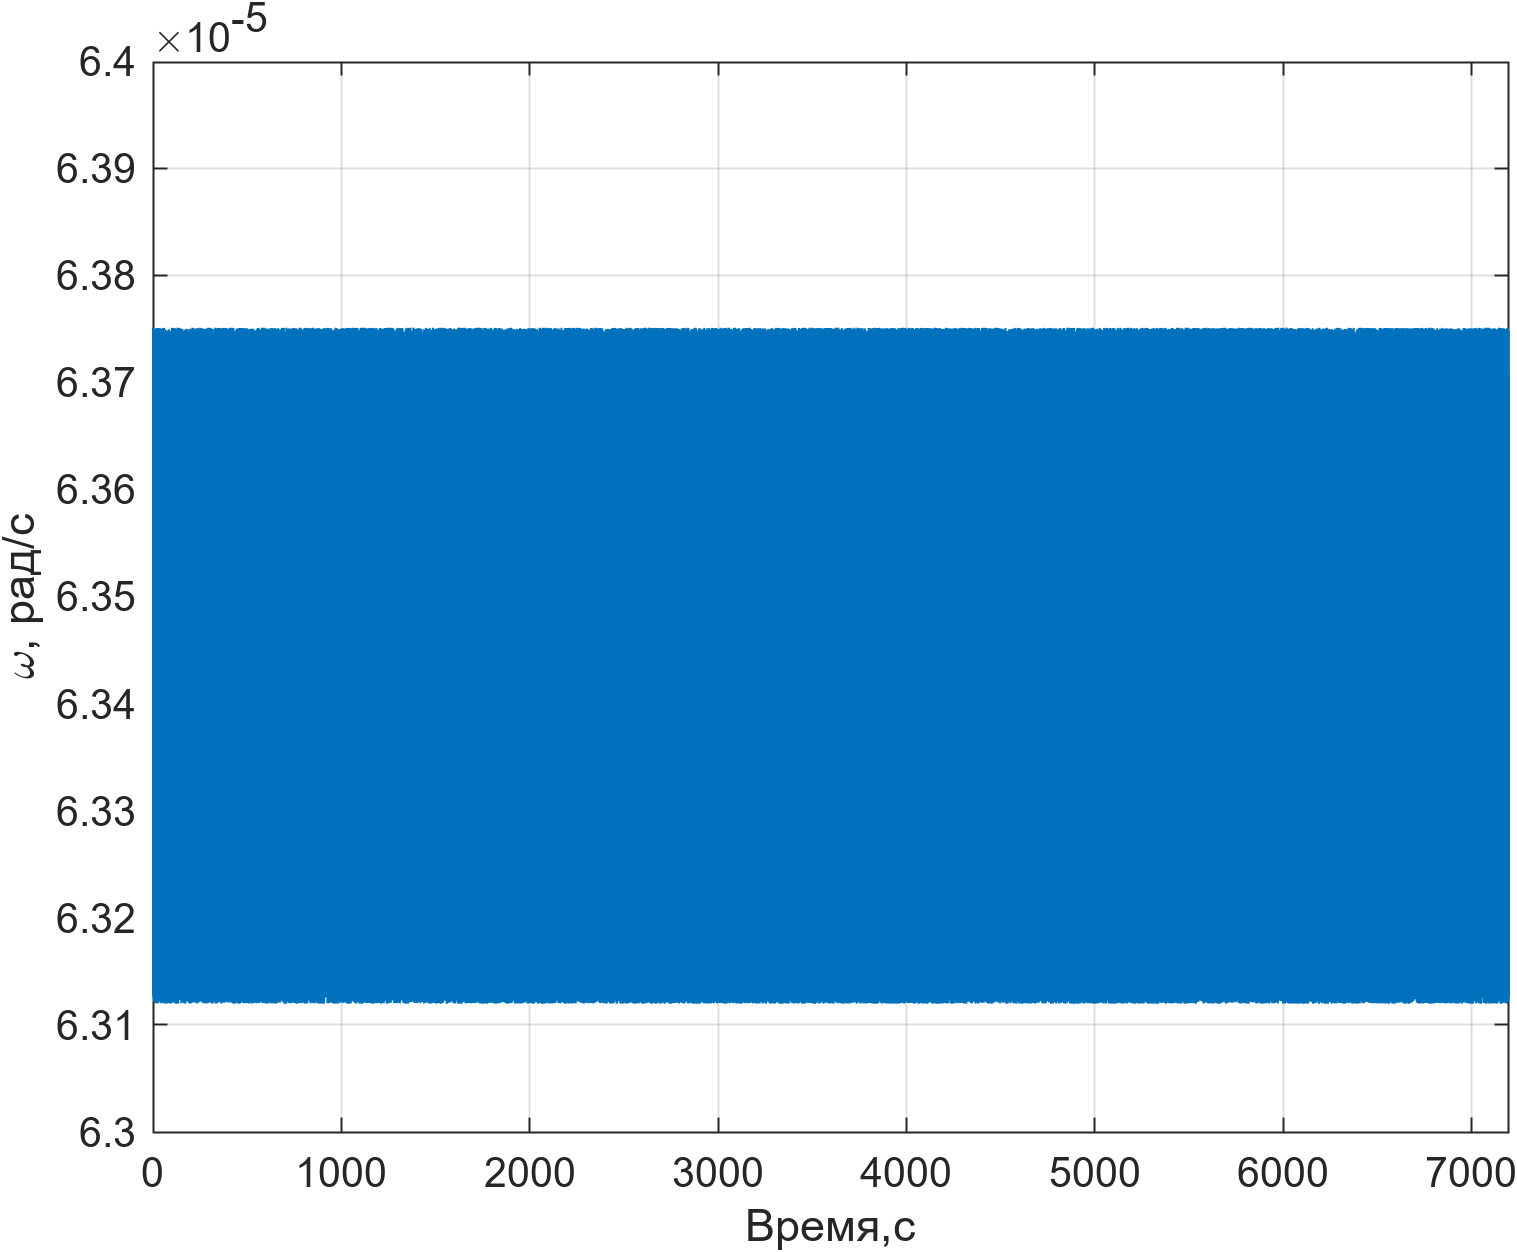
\includegraphics[scale=0.8]{matlab/gyroEarth.png}}
	\caption{Измерение проекции угловой скорости вращения Земли}
	\label{fig:Earth}
\end{figure}

Математическое ожидание сигнала гироскопа:
\begin{equation}
	\bar{\omega}
	= \frac{1}{N}\sum_{i=1}^{N}\omega_g(t_i).
	\label{eq:mean}
\end{equation}

По расчетам среднее значение составляет 
$
\bar{\omega} = \SI{6,34 e-5}{\text{рад/c}}
$

Угловая скорость вращения Земли
$\Omega_E = 2\pi/T_{\text{сут}}\approx \SI{7,292 e-5}{\text{рад/с}}.
$
На широте города Санкт-Петербург $\phi_{\mathrm{e}} = 59^\circ57'$ получаем проекцию на вертикальную ось гироскопа:
\[
\omega_e
= \Omega_E\sin\phi_{\text{e}}
\approx 7.292\cdot10^{-5}\sin(59^\circ57')
\approx 6.32\times10^{-5}\text{рад/с}.\\
\]

Смещение нуля:
\begin{equation}
	\epsilon
	= \bar{\omega} - \omega_e = \SI{3,16 e-7}{\text{рад/c}}.
	\label{eq:omega_correct}
\end{equation}

Оценка шумовой составляющей. Дисперсия определяется по формуле:
\begin{equation}
	\sigma^2=\frac{1}{N-1}\sum_{i=1}^N(\omega_i-\bar{\omega})^2.
	\label{eq:disperssion}
\end{equation}

Дисперсия составляет: $\sigma^2=\SI{3,15 e-7}{\text{рад/c}} \approx \SI{0,006}{^\circ /c}$

Итоговая погрешность измерения угловой скорости определяется по формуле:
\begin{equation}
	\Delta_{\omega}=\sqrt{\epsilon^2+\sigma^2}=\SI{3,645 e-7}{\text{рад/c}}.
	\label{eq:rmse}
\end{equation}

Для измерений нам требуется угловое ускорение, которое определяется как:
\begin{equation}
	\alpha =\frac{\omega_i-\omega_{i-1}}{\Delta t}.
	\label{eq:acc}
\end{equation}
Ошибка измерения составляет:
\begin{equation}
	\Delta_\alpha = \frac{\sqrt{2}\sigma}{\Delta t} = \SI{2,57 e-5}{\text{рад}/c^2}.
	\label{eq:rmse_a}
\end{equation}







Непосредственно перед измерениями контролируются условия окружающей среды. Температура воздуха в помещении должна находиться в пределах 15–35 °С, относительная влажность — 45–80 \%, атмосферное давление — 84–107 кПа. Контроль осуществляется с помощью барометра-анероида и психрометра. Соблюдение указанных параметров исключает влияние климатических факторов на точность эксперимента. Необходимые средства измерений представлены в таблице ~\cref{tab:measures}

\begingroup
\small
\captionsetup[table]{skip=7pt}

\begin{longtable}{|>{\raggedright\arraybackslash}p{5cm}|
		>{\raggedright\arraybackslash}p{8cm}|
		>{\raggedright\arraybackslash}p{3cm}|}
	\caption{Средства измерений}\label{tab:measures}\\[-0.45\onelineskip]
	\hline
	\textbf{Наименование} & \textbf{\raggedright Метрологические и технические характеристики} & \textbf{\raggedright Измеряемая величина} \\
	\hline
	\endfirsthead
	
	\caption*{Продолжение таблицы~\thetable}\\[-0.45\onelineskip]
	\hline
	\textbf{Наименование} & \textbf{Метрологические и технические характеристики} & \textbf{Измеряемая величина} \\
	\hline
	\endhead
	
	\hline
	\endfoot
	
	\hline
	\endlastfoot
	
	Барометр-анероид метрологический БАММ-1 \newline(№ ФИФ ОЕИ 10069-11)
	& Диапазон измерений давлений от 80 до \SI{106}{\kilo\pascal} (от 600 до \si{800\text{~мм рт. ст.}})
	Пределы допускаемой основной погрешности после введения поправок из паспорта $\pm\SI{0,2}{\kilo\pascal}$ ($\pm \si{1,5\text{~мм рт. ст.}}$)
	& Атмосферное давление            \\ \hline
	
	Психрометр аспирационный МВ-4-2М \newline(№ ФИФ ОЕИ 10069-11)
	& Диапазон измерения температуры: \newline от минус 25 до \SI{50}{\degreeCelsius};\newline Пределы допускаемой погрешности измерений температуры не более $\pm \SI{0,1}{\degreeCelsius}$; \newline Диапазон измерений относительной влажности: от 10 до 100 \%.
	& Относительная влажность воздуха, температура \\ \hline
	
	Преобразователь угловых перемещений ЛИР-ДА190К \newline(№ ФИФ ОЕИ 80050-20)
	& Диапазон измерений от 0 до \SI{360}{\degree}; \newline Пределы допускаемой абсолютной погрешности измерений: $\pm10 "$.
	& Угол разворота \\ \hline
	
	Штангенциркуль ШЦЦ-I-125-0,01
	\newline (№ ФИФ ОЕИ 81768-21)
	& Диапазон измерения от 0 до 125 мм; Шаг дискретности цифрового отсчётного устройства $\SI{0,01}{\milli\meter}$; Пределы допускаемой абсолютной погрешности $\SI{\pm0,03}{\milli\meter}$.
	& Геометрические размеры маховика\\ \hline
	
	Осциллограф TDS1012B \newline (№ ФИФ ОЕИ 32618-06) 
	& Диапазон установки коэффициентов отклонения 10 $\si{\text{мВ/дел - }5\text{В/дел.}}$
	\newline Погрешность установки коэффициентов отклонения: $\pm3$ \%.
	\newline Диапазон коэффициента развёртки $\si{5\text{нс/дел}-50\text{с/дел.}}$
	\newline Пределы допускаемой абсолютной погрешности измерения временных интервалов: $\pm(K_p/250+50 \cdot10^{-6}\cdot T + 0,6 )$, где \(K_p\) "---коэффициент развёртки, \(T\) "---измеряемый временной интервал, с.
	&Временные  интервалы\\ \hline
	
	
	Весы электронные EK-12Ki
	\newline (ФИФ ОЕИ 25312-03)
	& Наибольший предел взвешиваний $\SI{12}{\kilogram}$; наименьший предел взвешиваний $\SI{20}{\gram}$; предел допускаемой погрешности $\SI{\pm3}{\gram}$.
	& Масса маховика\\ \hline
	
	Волоконно-
	\newline оптический гироскоп ОИУС-1000
	&Диапазон измеряемой угловой скорости: $\SI{\pm550}{\degree\per\second}$.
	\newline Случайная составляющая нулевого сигнала при постоянной температуре при осреднении 100 секунд не более $\SI{0,01}{\degree\per\hour}$.
	\newline Случайная составляющая нулевого сигнала в диапазоне рабочих температур при скорости изменения температуры $\SI{0,4}{\degreeCelsius\per\minute}$ не более $\SI{0,1}{\degree\per\hour}$.
	\newline Погрешность измерения угловой скорости не более $0,01$ \%.
	&Угловая скорость	\\ \hline
	
\end{longtable}
\normalsize
\endgroup








\subsection{Определение тестового момента}

Для задания эталонного воздействия на подвес используется тестовый маховик, установленный на отдельном приводе. 

При подаче напряжения на двигатель маховик начинает вращение по заданному закону изменения угловой скорости. Управляющая система обеспечивает трапецеидальный профиль разгона, что позволяет выделить участок равномерного ускорения. Профиль разгона показан на рисунке ~\cref{fig:flyweel_speed}.

\begin{figure}[!h] 
	\centerfloat{
		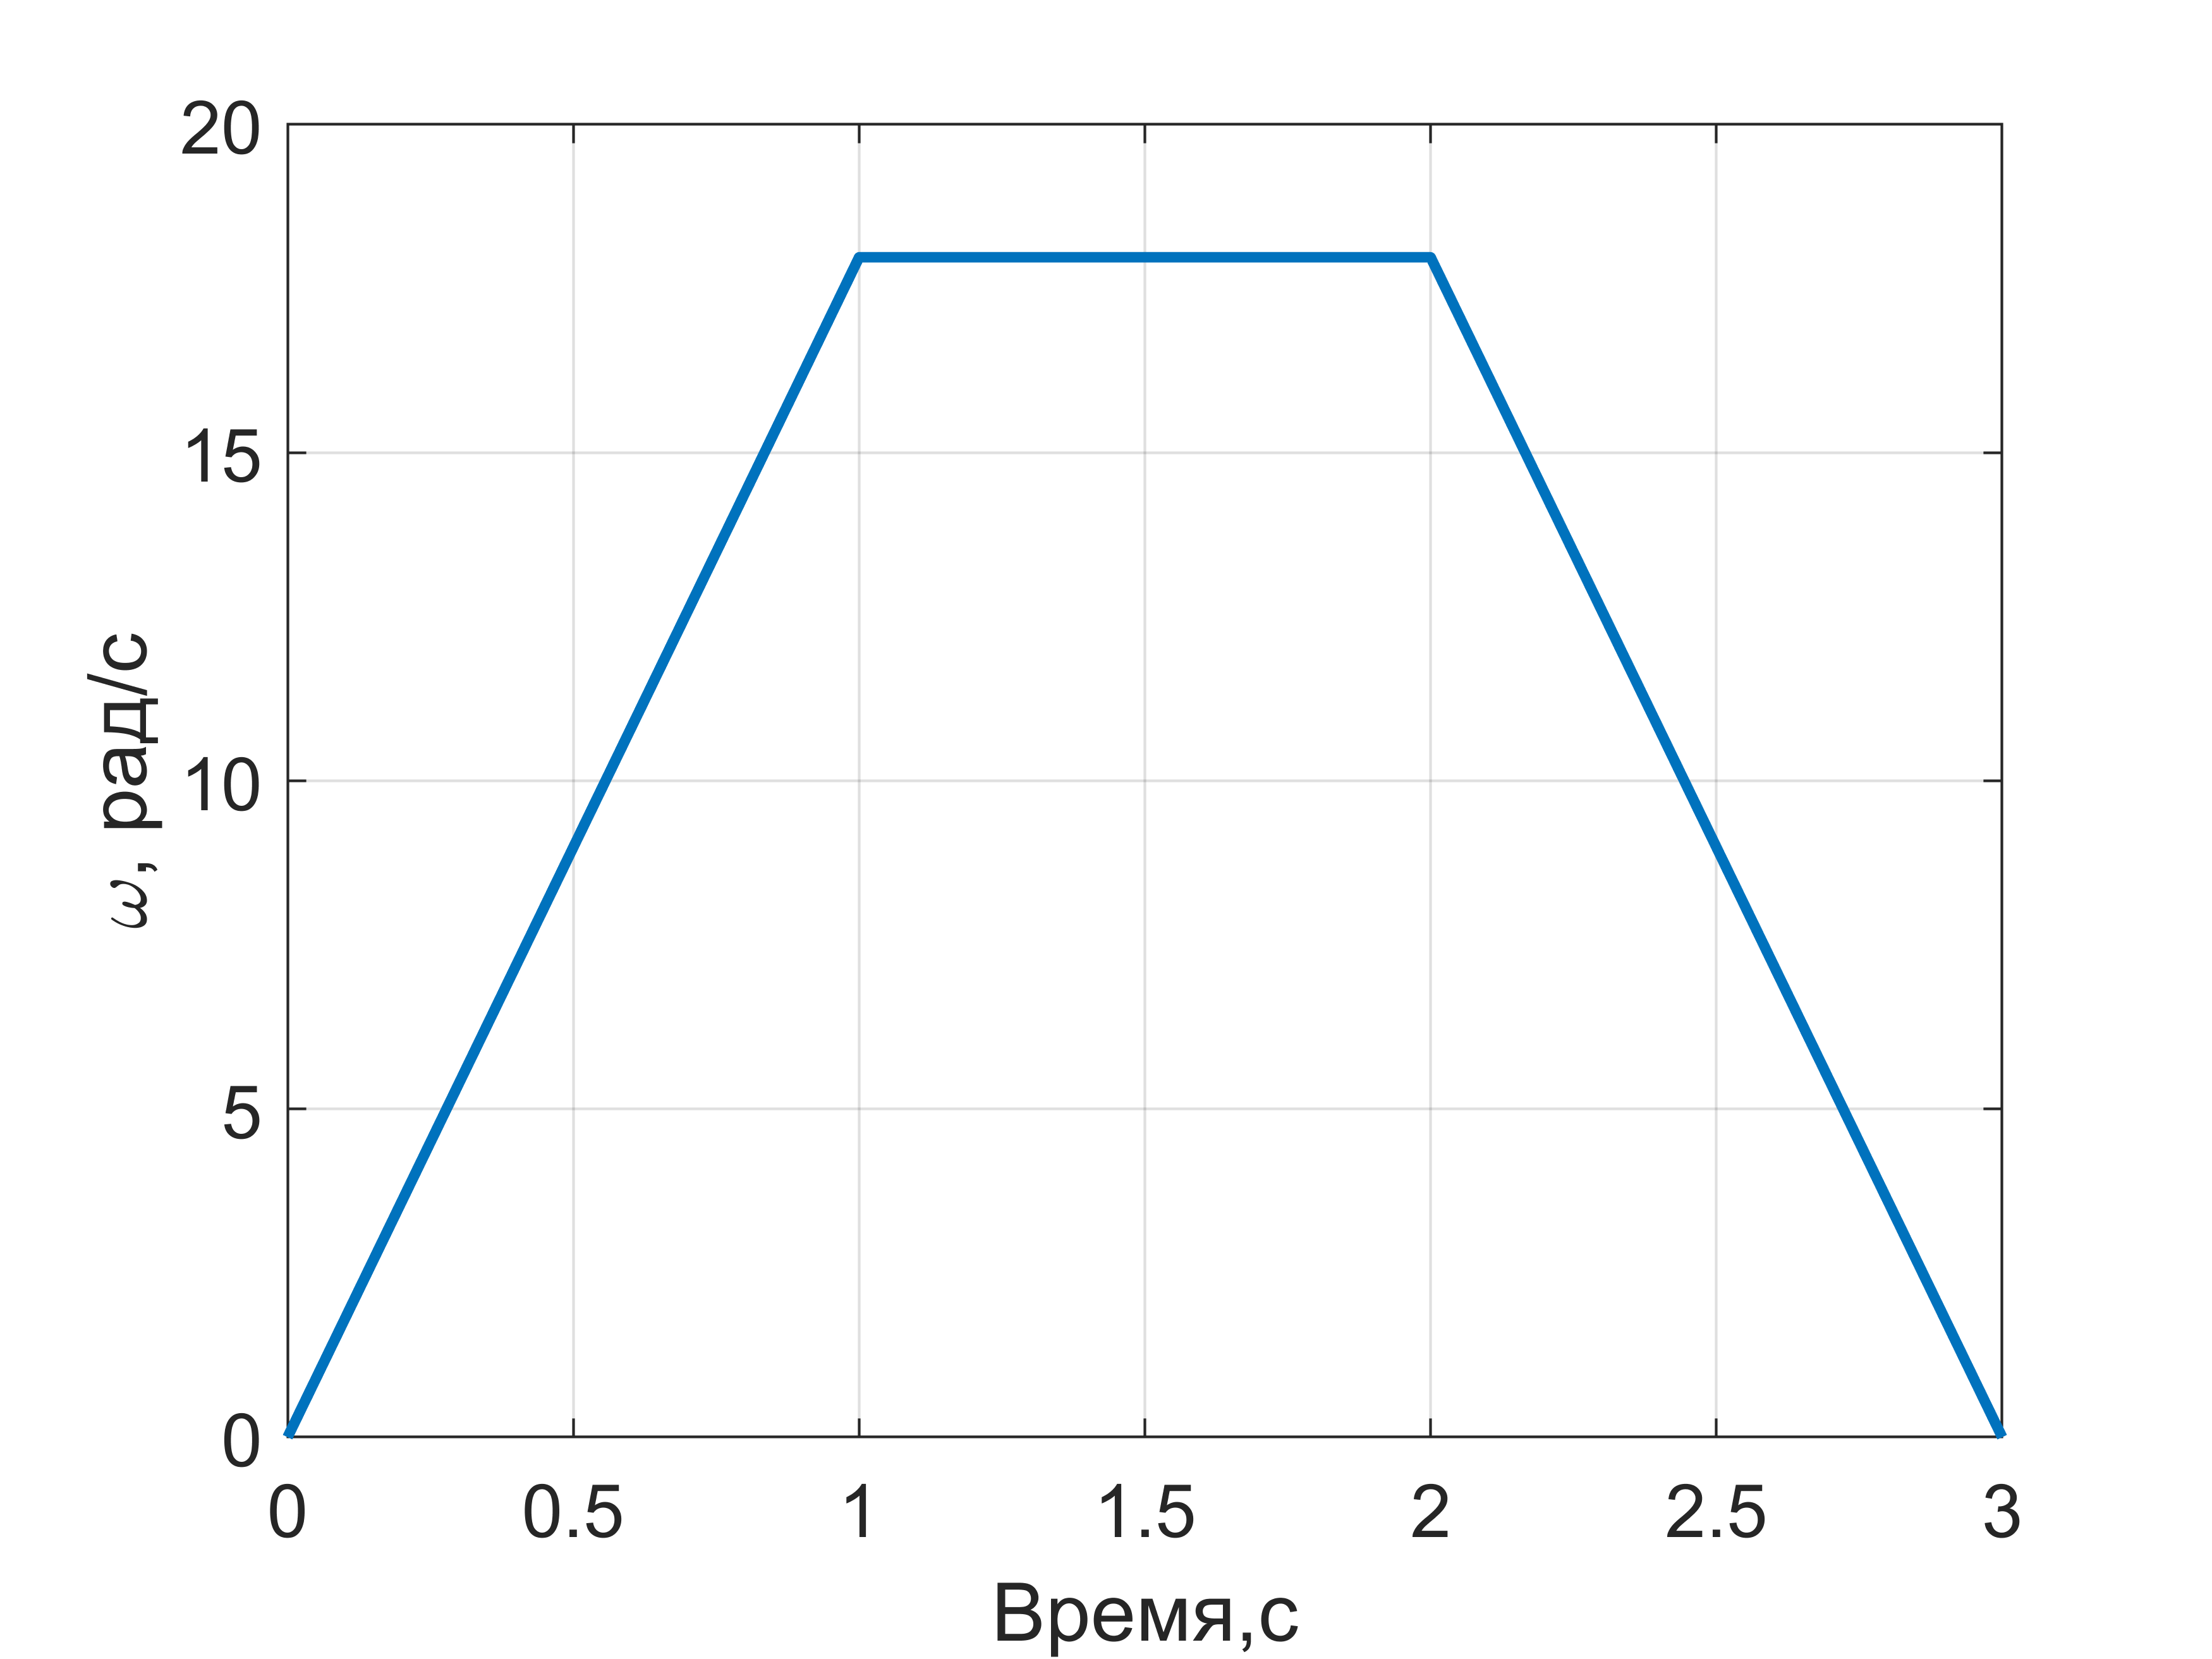
\includegraphics[scale=0.8]{matlab/img/flyweel_profile.png} 
	}
	\caption{Профиль разгона тестового маховика}
	\label{fig:flyweel_speed} 
\end{figure}



Скорость вращения определяется с помощью преобразователя угловых перемещений ЛИР-ДА190К. Угловая скорость определяется как отношение поворота маховика на угол $2\pi$ радиан к интервалу времени между двумя последовательными импульсами $t_{i+1}, t_i$ преобразователя: 

\begin{equation}
	\label{eq:flyweel_spd}
	\omega_i=\frac{2 \pi}{(t_{i+1}-t_i)},
\end{equation}
где \(i=1...5\) --- номер импульса.

Осциллограмма сигнала преобразователя представлена на рисунке ~\cref{fig:encoder}


\begin{figure}[!h] 
	\centerfloat{
		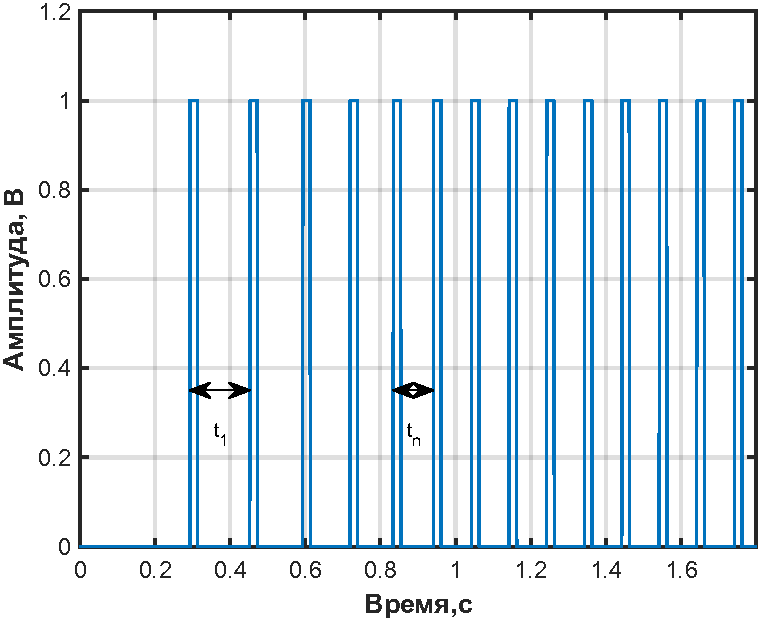
\includegraphics[scale=1]{matlab/img/encoder.pdf} 
	}
	\caption{Осциллограмма сигнала преобразователя угловых перемещений}
	\label{fig:encoder} 
\end{figure}

Угловое ускорение определяется как:

\begin{equation}
	\label{eq:flyweel_acc}
	\varepsilon = \frac{\omega_k-\omega_1}{t_k-t_1},
\end{equation}
где \(\omega_1, \omega_k\) --- начальная и конечная угловая скорость на участке разгона, \(t_1, t_k\) --- соответствующие моменты времени.

\subsection{Оценка бюджета погрешности}

Полный бюджет неопределённости формируется через разложение всех источников ошибок и последующее вычисление их вклада в итоговую величину измеряемого тестового момента. Момент инерции маховика $J_m$ определяется один раз при сборке стенда на основе геометрических размеров и массы маховика. Измерения выполняются с использованием аттестованных средств измерений (штангенциркуля и весов), что гарантирует соответствие требованиям метрологического контроля. Погрешность измерения момента инерции составляет $\Delta J = 4.58 \cdot 10^{-7}\,\text{кг}\cdot\text{м}^2$ Подробный расчёт момента инерции приведён в приложении ~\ref{app:A}.

Для измерения углового ускорения маховика использовался преобразователь угловых перемещений, установленный на валу. Преобразователь имеет паспортную погрешность $\Delta \phi = 10" = 4,85 \cdot 10^{-5} \text{~рад}$.

Маховику задается угловое ускорение $\epsilon = 18.65 \,\text{рад/с}^{2}$. Измерение ускорения осуществляется косвенным методом --- через определение второй производной углового положения:

\begin{equation}
	\epsilon = \frac{d^{2}\varphi}{dt^{2}}.
\end{equation}

На практике вычисление производной производится численно по результатам дискретных измерений. При использовании центральной разности второго порядка для временного шага $\Delta t$ получаем:

\begin{equation}
	\epsilon(t) \approx \frac{\varphi(t + \Delta t) - 2\varphi(t) + \varphi(t - \Delta t)}{\Delta t^{2}}.
\end{equation}

Так как все измерения угла имеют погрешность $\Delta \phi$, она вносит вклад в неопределённость ускорения. При независимых ошибках трёх точек формула для стандартной неопределённости ускорения принимает вид:

\begin{equation}
	u_{\epsilon} = \frac{\sqrt{6}\,u_{\varphi}}{\Delta t^{2}},
\end{equation}
где \(u_\epsilon\)"--- стандартная неопределённость измерения угла.

Если паспортная величина $\pm10"$ задаётся как предел допускаемой абсолютной ошибки при равномерном распределении, то стандартная неопределённость:

\begin{equation}
	u_{\varphi} = \frac{\Delta \varphi}{\sqrt{3}} 
	\approx \frac{4.85 \cdot 10^{-5}}{\sqrt{3}} 
	\approx 2.8 \cdot 10^{-5} \,\text{рад}.
\end{equation}

Таким образом, итоговая погрешность ускорения зависит от выбранного временного интервала дискретизации $\Delta t$. В работе выбран шаг $\Delta t = \SI{0,02}{\second}$:

\begin{equation}
	u_{\epsilon} = \frac{\sqrt{6} \cdot 2.8 \cdot 10^{-5}}{(0.02)^{2}}
	\approx 0.171 \,\text{рад/с}^{2}.
\end{equation}

Переходя от ускорения к моменту, отметим, что измеряемая величина задаётся произведением

\begin{equation}
	M = J \cdot \epsilon,
\end{equation}
а потому полная стандартная неопределённость момента, при независимости вкладов $J$ и $\alpha$, определяется законом распространения погрешностей:

\begin{equation}
	u_{M} = \sqrt{\left(\epsilon \Delta J\right)^{2} + \left(J u_{\alpha}\right)^{2}}.
\end{equation}

Подставляя числовые значения получим:

\begin{equation}
	u_{M} \approx \sqrt{(8.54 \times 10^{-6})^{2} + (4.61 \times 10^{-5})^{2}}
	\approx 4.7 \times 10^{-5} \,\text{Н·м}.
\end{equation}

Для полноты оценим и сам момент:

\begin{equation}
	M = J \epsilon = 2.69 \times 10^{-4} \cdot 18.65 
	\approx 5.02 \times 10^{-3} \,\text{Н·м},
\end{equation}
а относительная неопределённость:

\begin{equation}
	\frac{u_{M}}{M} \approx 
	\frac{4.68 \times 10^{-5}}{5.02 \times 10^{-3}}
	\approx 0.93\% .
\end{equation}

Разработанный стенд прошёл метрологическую аттестацию в установленном порядке. 
Аттестация выполнена АО «НПО Техномаш» имени С.~А.~Афанасьева при поддержке 
Госкорпорации «Роскосмос». По результатам процедуры выдано свидетельство 
№~030-500/2024-61 (РОСС RU.0001.310066/2024), зарегистрированное в государственном 
реестре под номером ФР.1.28.2024.49055.

Методика измерения некомпенсированного возмущающего момента признана 
соответствующей требованиям ГОСТ~Р~8.563--2009. Диапазон измеряемых значений 
составляет от $10^{-3}$ до $1 \,\text{Н}\cdot\text{м}$.  

Таким образом, стенд обеспечивает требуемую точность измерений 
и может быть использован в качестве средства поверки и исследований 
оптико-механических систем. %Сертификат аттестации представлен в приложении ~\cref{app:certificate}

	
\section{Измерение реактивного момента оптико-механической системы}

После установки изделия в изделиедержатель подвесная система переводится в состояние покоя. Для этого фиксируют платформу в исходном положении и ожидают затухания переходных процессов до уровня, при котором остаточные колебания не превышают допустимой амплитуды (менее 1 \% от диапазона гироскопа).

Задаётся эталонный момент с помощью тестового маховика. Скорость колебаний регистрируется гироскопом с частотой дискретизации $f_s=\SI{100}{\hertz}$. Для уменьшения случайных составляющих, измерения повторяются 10 раз. Усреднённый массив угловой скорости вычисляется по формуле:

\begin{equation}
	\label{eq:mean_spd}
	\overline{\omega_{i}}=\frac{1}{N}\sum_{j=1}^{N}\omega_{i}^{(j)}, \qquad N = 10,
\end{equation}
где \(\omega_{i}^j\) --- значение угловой скорости в $i-$ой точке при $j-$ом повторе.

Из усреднённого массива вычисляется угловое ускорение методом численного дифференцирования:

\begin{equation}
	\label{eq:mean_acc}
	\varepsilon_{i}
	= \frac{\overline{\omega}_{i+1}-\overline{\omega}_{i}}{\Delta t},
	\qquad
	\Delta t = \frac{1}{f_s}.
\end{equation}

На участке равноускоренного движения определяется среднее значение ускорения:


\begin{equation}
	\label{eq:acc}
	\varepsilon_m = \frac{1}{n}\sum_{i=1}^{n} \varepsilon_{i},
\end{equation}
где \(n\) --- число отсчётов на участке равномерного ускорения.

После задания эталонного момента выполняется измерение реактивного момента исследуемой ОМС. Привод изделия осуществляет поворот подвижной части на заданный угол. Под действием реактивного момента подвес совершает колебания, скорость которых  регистрирует гироскоп.

Данные обрабатываются аналогично: формируется усреднённый массив скорости колебаний:

\begin{equation}
	\label{eq:omega_op}
	\overline{\omega_{o_i}}
	= \frac{1}{N}\sum_{j=1}^{N} \omega_{o_i}^{(j)}.
\end{equation}

После выполняется численное дифференцирование:

\begin{equation}
	\label{eq:epsilon_op}
	\varepsilon_{o_i}
	= \frac{\overline{\omega}_{o_i+1}
		- \overline{\omega}_{o_i}}{\Delta t}.
\end{equation}

Среднее ускорение на равноускоренном участке находится как:

\begin{equation}
	\label{eq:epsilon_op_mean}
	\varepsilon_{o}
	= \frac{1}{n}\sum_{i=1}^{n} \varepsilon_{o_i}\,.
\end{equation}

Искомый остаточный реактивный момент рассчитывается через соотношение:

\begin{equation}
	\label{eq:Mom}
	M_o = M_m \cdot \frac{\varepsilon_o}{\varepsilon_m}.
\end{equation}

Окончательное значение реактивного момента определяется как максимальное по модулю среди положительного и отрицательного экстремумов:

\begin{equation}
	\label{eq:Mom}
	M_{max} = max\{|M^+|, |M^-|\}.
\end{equation}






\section*{Выводы по главе 3}

В данной главе разработан и создан испытательный стенд для измерения остаточных реактивных моментов оптико-механических систем.  
Построена теоретическая модель стенда в виде колебательного звена, что позволило определить требования к собственным частотам и декременту затухания подвесной системы. На основе анализа выбрана конструкция со струной в качестве упругого элемента, обеспечивающая малый уровень диссипативных потерь и одну степень свободы для исследуемого изделия.

Стенд оснащён волоконно-оптическим гироскопом для регистрации угловых колебаний и тестовым маховиком с известным моментом инерции для формирования эталонного воздействия. Разработана методика измерений, включающая юстировку подвесной системы, контроль климатических параметров и процедуры определения тестового момента. Проведена оценка бюджета погрешности, показавшая, что основными источниками неопределённости являются точность задания углового ускорения и погрешность измерения момента инерции маховика.

Созданный комплекс прошёл метрологическую аттестацию в установленном порядке, что подтверждает его пригодность для практического применения. Диапазон измеряемых значений составил от $10^{-3}$ до $1 \,\text{Н}\cdot\text{м}$ при относительной погрешности не более 1 \%. Это обеспечивает возможность достоверного определения остаточных реактивных моментов при испытаниях оптико-механических систем.

Таким образом, в работе сформирован базис для последующих экспериментальных исследований влияния реактивных моментов на смаз и качество изображений. 



\clearpage
\FloatBarrier           % Глава 3
\chapter{Глава 4}\label{ch:ch4}

\section{Устройство относительного измерения момента}\label{sec:ch4/sect1}


В филиале АО «Корпорация «Комета» – «НПЦ ОЭКН» создано и и аттестовано устройство относительного измерения остаточного момента (УОИОМ). На рисунке \cref{fig:yoim} представлен общий вид установки.

\begin{figure}[ht]
	\centerfloat{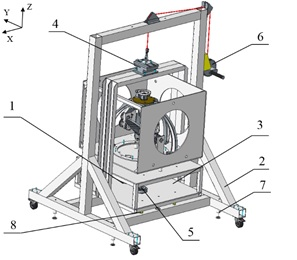
\includegraphics[scale=2]{yoiom}}
	\caption{Устройство относительного измерения остаточного момента}
	\legend{1 – маховик; 2 – платформа; 3 – измерительная платформа с изделиедержателем; 4 – зацеп настраиваемый; 5 – узел привода редукторного OZ; 6 – привод редукторный OZ;
	 7 – волконно-оптический гироскоп; 8 – конус}
	\label{fig:yoim}
\end{figure}

Стенд для измерения остаточного реактивного момента представляет собой конструкцию, обеспечивающую измеряемой аппаратуре одну степень свободы, без сухого трения. В процессе углового перемещения ОМС на основание аппаратуры действует реактивный момент. Частично этот момент компенсируется маховиками, входящими в состав ОМС. Таким образом,
стенд служит для измерения некомпенсированного внутренними средствами аппаратуры реактивного момента. Конструктивно стенд представляет собой 
крутильный маятник. Момент инерции маятника состоит из суммы моментов инерции рамы с кантователем и момента инерции аппаратуры по измеряемой оси. Кантователь входит в узел подвеса и служит для удобства 
смены измеряемой оси аппаратуры путем расположения этой оси строго вертикально по оси чувствительности подвеса. Дифференциальное уравнение колебательного звена крутильного маятника запишем  в виде [13]

\begin{samepage}
	\begin{equation}
		\label{eq:eq_yoimDiff}
		\begin{alignedat}{2}
			J\ddot{\phi}\left(t\right) + 2b\dot{\phi}\left(t\right)+c\phi\left(t\right) = M\left(t\right)
		\end{alignedat}
	\end{equation}
	\begin{align*}
		\text{где}	& \quad J - \textnormal{момент инерции;}\\           
		& \quad b - \textnormal{обобщённое вязкое трение;}        \\
		& \quad c -  \textnormal{угловая жесткость подвеса;} \\
		& \quad M(t) - \textnormal{внешний момент;}         \\
		& \quad \phi(t) -\textnormal{угол порота узла подвеса} \\
	\end{align*}
\end{samepage}

Запишем уравнение~\cref{eq:eq_yoimDiff} иначе:ъ

\begin{samepage}
	\begin{equation}
		\label{eq:eq_yoimDiff2}
		\begin{alignedat}{2}
			\phi\left(t\right)+2\xi\phi\left(t\right)+\omega_{0}^2\phi\left(t\right) = M\left(t\right)/J
		\end{alignedat}
\end{equation}
\begin{align*}
	\text{где}	& \quad \omega_0 - \textnormal{собственная частота колебательного звена;}\\           
	& \quad \xi - \textnormal{декремент затухания;}        \\
\end{align*}
\end{samepage}


На рисунке~\cref{fig:amplitude-freq-char} представлены логарифмические амплитудная и фазовая характеристики колебательного звена. Характеристики построены относительно резонансной (собственной) частоты.

\begin{figure}[ht]
	\centerfloat{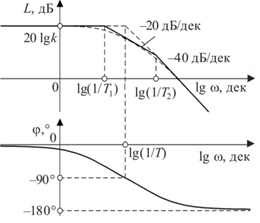
\includegraphics[scale=2]{amplitude-freq-char}}
	\caption{ЛАЧХ колебательного звена}
	\label{fig:amplitude-freq-char}
\end{figure}


Как видно из рисунка, колебательное звено не искажает входного сигнала ни по амплитуде вплоть до области, близкой к собственной частоте колебаний. В области частот выше собственной выходной сигнал подавляется с темпом \SI{-40}{\text{дБ/декада}}, а фаза выходного сигнала сдвигается на $\pi$ по отношению к фазе входного входного сигнала[14]. Если выходной сигнал состоит из нескольких гармоник, то в этой области частот высокочастотные гармоники будут ослабляться по мере удаления от частоты резонанса. Таким образом, с точки зрения информативности измерений наиболее рационально работать в дорезонансной области частот, где угловые перемещения узла подвеса наилучшим образом соответствуют действию моментов на узел подвеса.

Зададим внешний момент в виде функции, представленной на рисунке~\cref{fig:external_moment}, и разложим её в ряд Фурье [15]



\begin{samepage}
	\begin{equation}
		\label{eq:furie}
		\begin{alignedat}{2}
		M(t) = \frac{4 \alpha}{\pi} \cos\left(\frac{\pi}{4}\right) \sin\left(\omega t\right) + \\
				1/3 \cos\left(\frac{3\pi}{4} \right) \sin\left(3\omega t \right) + \\
				1/5 \cos \left(\frac{5 \pi}{4} \right) \sin \left(5 \omega t\right) + \\
				1/7 \cos \left(\frac{7 \pi}{4} \right) \sin \left(7 \omega t \right) + \\
				1/9 \cos \left(\frac{9 \pi}{4} \right) \sin \left(9 \omega t \right)+ ...
		\end{alignedat}
	\end{equation}
	\begin{align*}
		\text{где}	& \quad \alpha - \textnormal{собственная частота колебательного звена;}\\           
	\end{align*}
\end{samepage}

На рисунке~\cref{fig:external_moment_furie} приведены упрощенный график остаточного реактивного, возникающего при тестовом воздействии маховика, и результат суммирования первых шести слагаемых ряда Фурье~\cref{eq:furie}. Пропустим шесть первых гармоник ряда Фурье через колебательное звено~\cref{eq:eq_yoimDiff} последовательно и суммируем полученные результаты. 

Для каждой из гармоник угла отклонения рамы стенда можно записать :

\begin{samepage}
	\begin{equation}
		\label{eq:diffur}
		\begin{alignedat}{2}
			\phi(t) + \psi \phi(t) + \omega_0^2 \phi(t) = \frac{M(t)}{J},
		\end{alignedat}
	\end{equation}
	\begin{align*}
		\text{где}	& \quad \alpha - \textnormal{собственная частота колебательного звена;}\\           
	\end{align*}
\end{samepage}

\todo{Формулы}


В соответствии с заданием на проектирование аппаратуры - первая гармоника возмущающего момента имеет период $T_1 = \SI{4}{c}~$(Время периода вращения оптической системы) и круговую частоту $\omega_{r_1} = \frac{1}{T_1} = \SI{0,25}{рад/c}$.

На рисунке~\cref{fig:decrement} приведен результат результат моделирования ускорения рамы под действием момента при различных настройках узла подвеса стенда с различными декрементами затухания и $T_1 = \SI{4}{c}$. На рисунке~\cref{fig:decrement} видно, что увеличение декремента затухания больше $\xi = 0,1$ приводит к существенным деформациям формы выходного сигнала по отношению к входному моменту. В стенде декремент затухания зависит от скоростного трения в оси подвеса и диссипативных потерь в металлической струне, на котором подвешена рама крепления ОМС. Следовательно, механические параметры струны и способ её крепления были выбраны таким образом, чтобы декремент затухания системы не превышал $\xi = 0,1$. 

Скорость качания узла подвеса измеряется волоконным оптическим гироскопом (ВОГ). После дифференцирования сигнала ВОГ получаем сигнал ускорения узла подвеса. Для получения значения момента на основание следует умножить полученное ускорение узла подвеса на момент инерции узла подвеса. 

Как следует из рисунка~\cref{fig:} для измерения моментов без существенных искажений следует настраивать узел подвеса на период собственных колебаний не менее 10-12 с.

В процессе измерений полученные значения ускорения сравниваются с ускорением, возникшим от воздействия измерительного маховика, который закрепляется на узле подвеса стенда.

Момент, вносимый измерительным маховиком $M_m$, определяется выражением

\begin{samepage}
	\begin{equation}
		\label{eq:final_moment}
		\begin{alignedat}{2}
			M_m=\frac{J_m\delta\omega_m}{\delta t},
		\end{alignedat}
	\end{equation}
где $J_m$ — расчётный момент инерции измерительного маховика, равный 
\SI{2.68e-4}{\kilogram\metre\squared}, определяется с относительной погрешностью 0,002, $\Delta \omega$ - разность скоростей участке линейного изменения скорости измерительного маховика,  $\Delta \omega=\SI{18,65}{\radian\per\second}$, $\Delta t$ -  шаг (дискрет) дискретизации по времени.
\end{samepage}



\begin{figure}[ht]
	\centering
	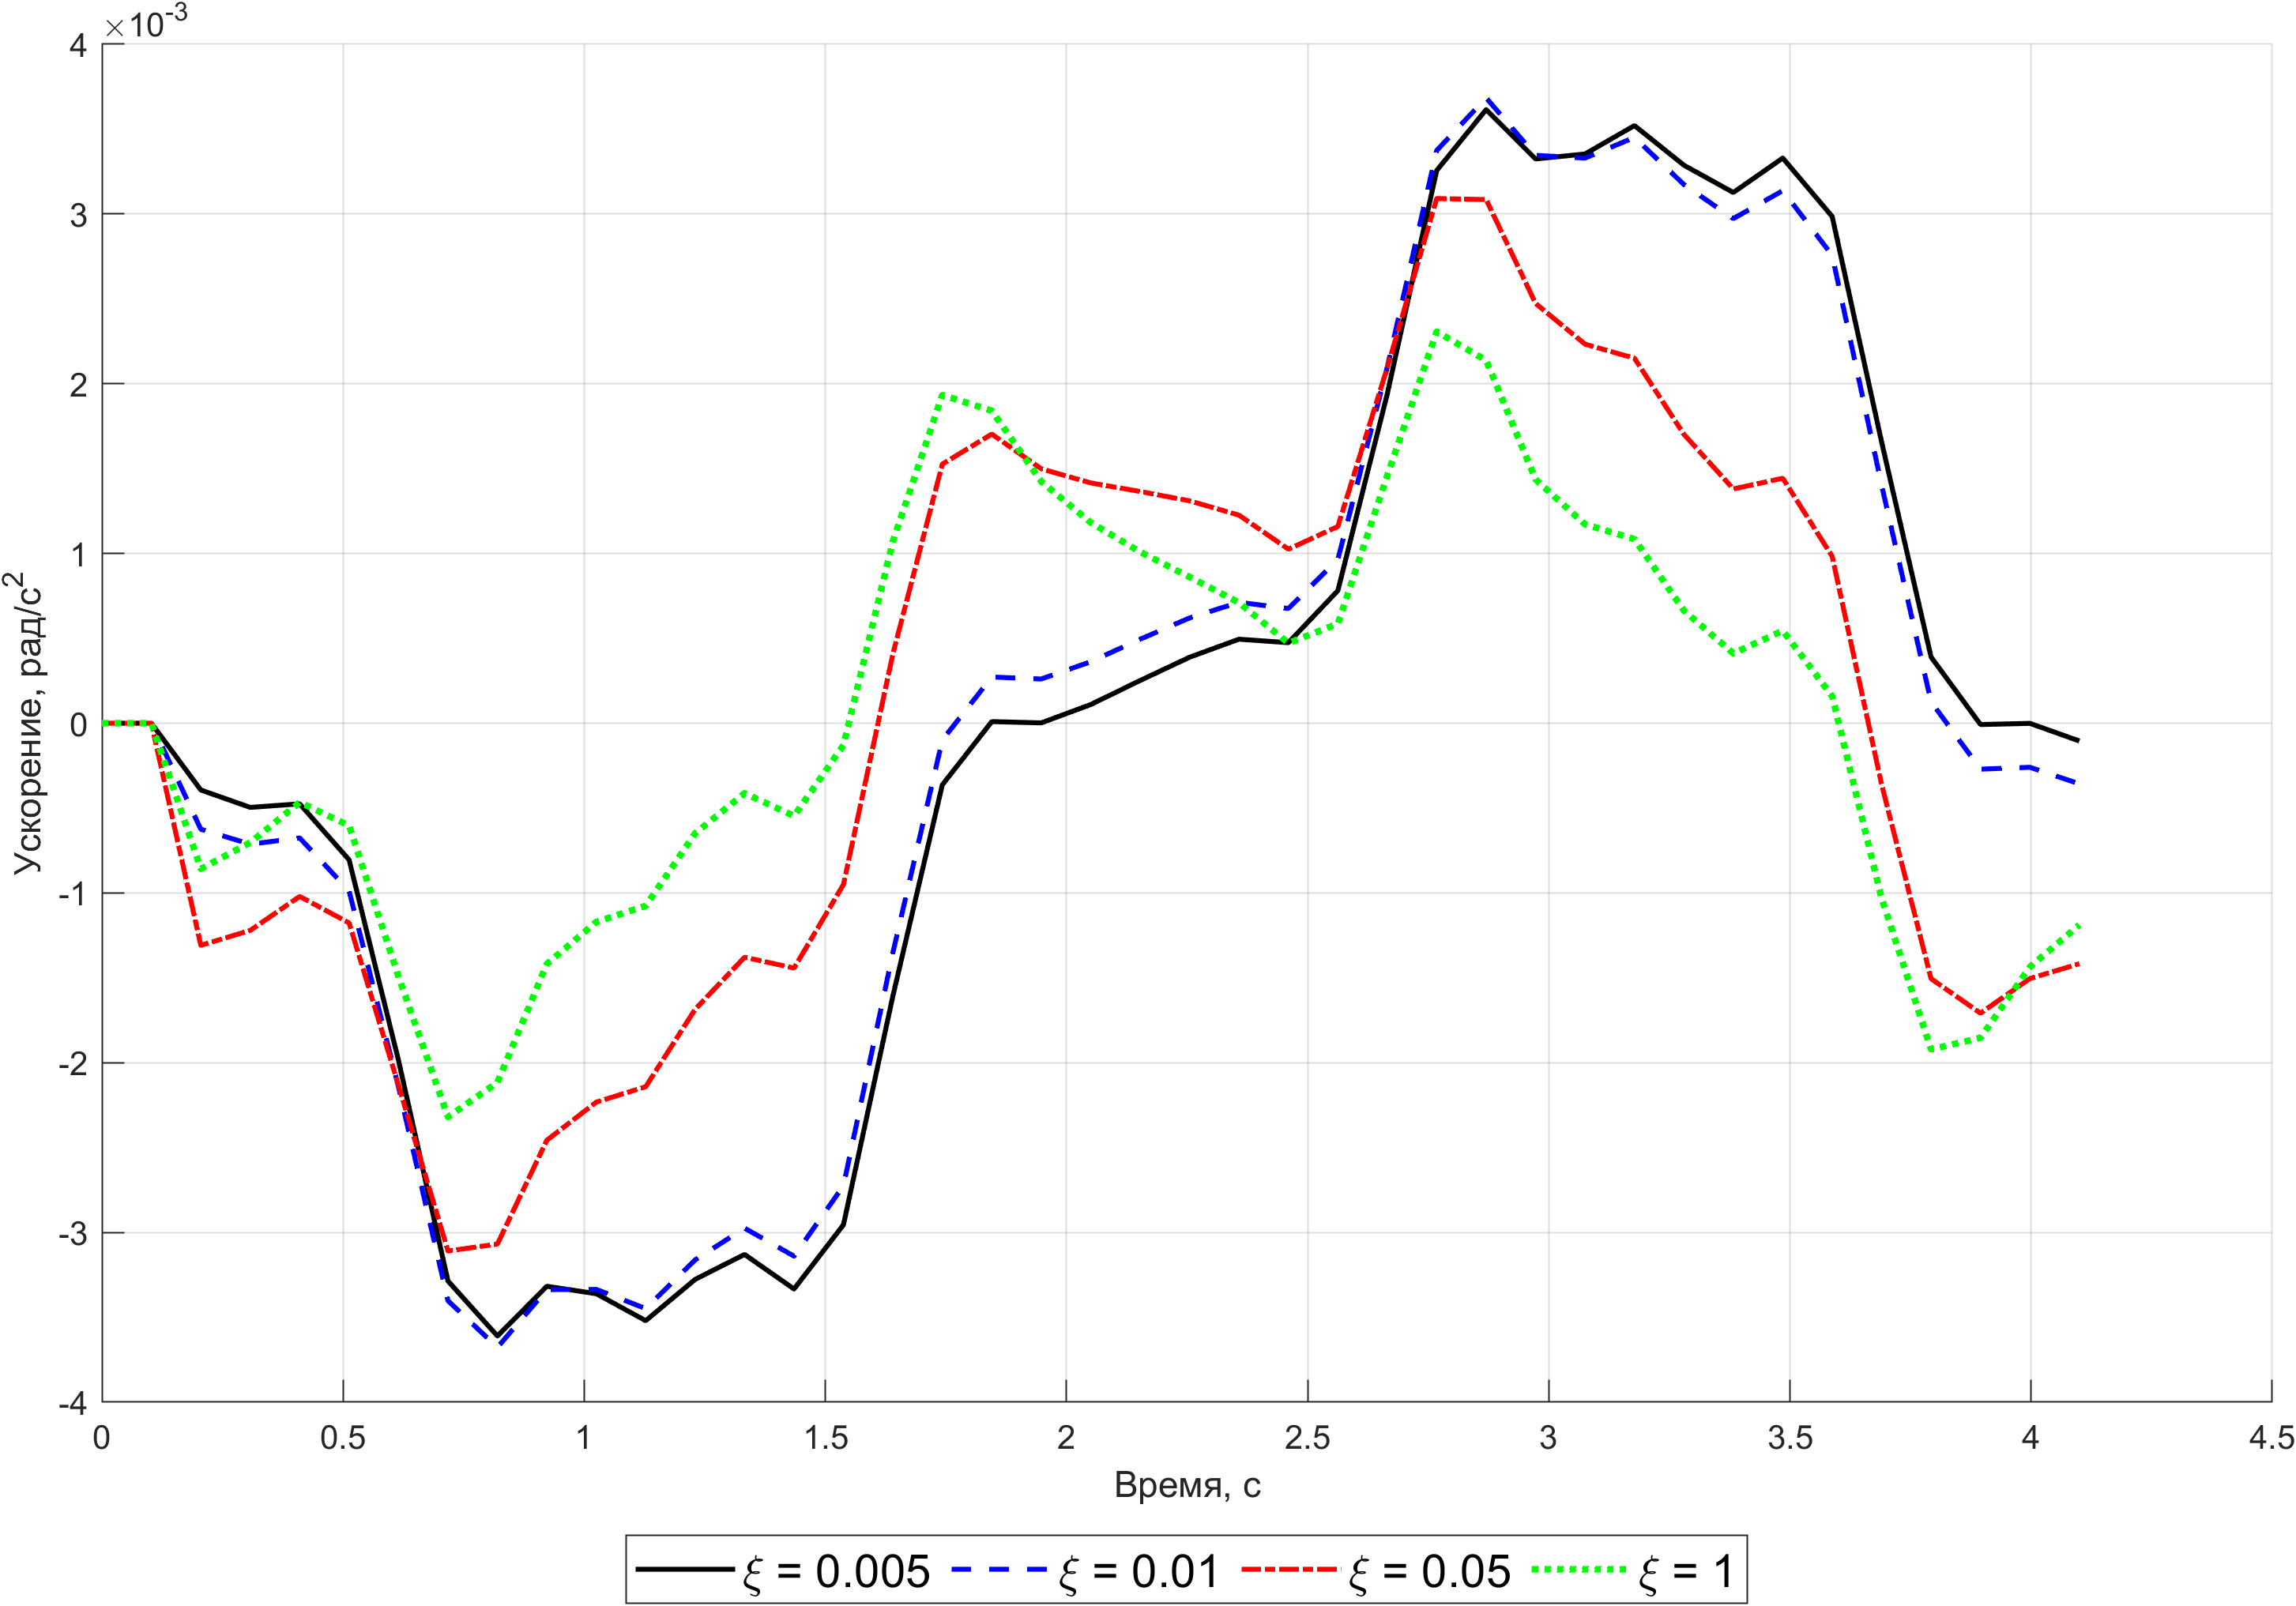
\includegraphics[scale=0.7]{matlab/decrement.png}
	\caption{Ускорение рамы с различными декрементами затухания}
	\label{fig:decrement}
\end{figure}

График, на рисунке~\cref{fig:test_moment} может служить основой для генерации задания контура управления по скорости вращения измерительного маховика.
\todo{Грфик}



\section{Конструкция стенда}\label{sec:ch4/sect2}

Стенд, показанный на рисунке~\cref{fig:yoim}, представляет собой подвешенный на тросе металлическом тросе куб, в который помещается исследуемая подвижная оптическая система. В качестве средств измерения используются датчик эталонного момента и ВОГ. Датчик эталонного момента состоит из моментного двигателя и маховик, суммарный момент инерции которых составляет \SI{2.68e-4}{\kilogram\metre\squared}.

\begin{figure}[ht]
	\centerfloat{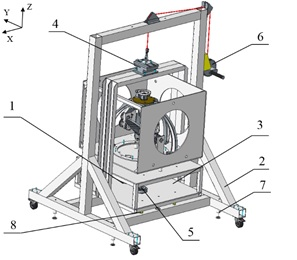
\includegraphics[scale=2]{yoiom}}
	\caption{Устройство относительного измерения остаточного момента}
	\legend{1 – маховик; 2 – платформа; 3 – измерительная платформа с изделиедержателем; 4 – зацеп настраиваемый; 5 – узел привода редукторного OZ; 6 – привод редукторный OZ;
		7 – волконно-оптический гироскоп; 8 – конус}
	\label{fig:yoim}
\end{figure}

Тестовое воздействие заключается в следующем. На двигатель-маховик подают управляющее напряжение, в результате чего он начинает вращаться по заранее заданному закону изменения угловой скорости. Угловые перемещения маховика измеряются преобразователем ЛИР-ДА190К. Крутящий момент от маховика передаётся на измерительную платформу с изделием-держателем, а скорость возникающих колебаний регистрируется волоконно-оптическим гироскопом.

В результате перемещения подвижной части изделия на основание стенда возникает крутящий момент, приводящий измерительную платформу с изделием-держателем в вынужденные колебания. Скорость этих колебаний фиксируется ВОГ.

Полученные показания подвергаются дифференцированию и последующей градуировке по эталонным значениям ускорения колебаний маховика, зарегистрированным при тестовом воздействии с заранее заданным кинетическим моментом.

В результате обработки данных определяется величина некомпенсированного крутящего момента, действующего на основание стенда при перемещении подвижной части ОМС. Пример полученных результатов измерений представлен на рисунке~\cref{fig:meauser_moment}.

\todo{график}

Абсолютная погрешность угломера ЛИР-ДА190К составляет
\[
\delta\varphi = 75''.
\]
При времени интегрирования
\[
t = 0{,}2\ \mathrm{с}
\]
это даёт погрешность угловой скорости
\[
\Delta\omega_m = \frac{\delta\varphi}{t}
= \frac{75''}{0,2\,\mathrm{s}}
= 0{,}1^\circ/\mathrm{s}
\approx 1{,}75\times10^{-3}\,\mathrm{c}^{-1}.
\]

Следовательно, относительная погрешность измерения угловой скорости маховика равна
\[
\delta_{\omega}
= \frac{\Delta \omega_m}{\omega_{\max}}
= \frac{1{,}75\times10^{-3}\,\mathrm{s}^{-1}}{18{,}65\,\mathrm{s}^{-1}}
\approx 9{,}38\times10^{-5}.
\]

% ------------------------------
% Погрешность измерения времени
% ------------------------------
Единица измерения времени \(\Delta t\) определяется числом тактовых импульсов контроллера за 1 с. При опорной частоте контроллера
\[
f_0 = 8000\ \mathrm{Гц}
\]
абсолютная погрешность измерения времени составляет
\[
\Delta t = \frac{1}{f_0} = 5\times10^{-4}\,\mathrm{s},
\]
что соответствует относительной погрешности не более
\[
\delta_t = \frac{\Delta t}{1\,\mathrm{s}} = 5\times10^{-4}.
\]

Эталонный момент на основание стенда от измерительного маховика $M_m=\SI{0,005}{Н\meter}$. Тогда требуемое значение ускорения $\frac{\Delta\omega_m}{\Delta t}$ измерительного маховика на линейном участке измерения скорости составит $\frac{\Delta\omega_m}{\Delta t} = \frac{M_m}{J_m}=\SI{18,65}{рад/c^2}$.

Таким образом основным источником погрешности при оценке остаточного момента на стенде является относительная погрешность гироскопа ВОГ ОИУС-1000 (0,01). Погрешность дискретизации времени $5 \cdot 10^{-4}$ по сравнению с этим пренебрежимо мала и увеличивает итоговую погрешность менее чем на 0,1 %.

Итоговая относительная погрешность измерений остаточного момента [16]

\begin{samepage}
	\begin{equation}
		\label{eq:final_moment_err}
		\begin{alignedat}{2}
			\delta M_m = \sqrt{(9,36 \cdot 10^{-5})^2+(1,9 \cdot 10^{-3})^2+(1\cdot 10^{-2})^2}
		\end{alignedat}
	\end{equation}
\end{samepage}

\section{Методика измерений}\label{sec:ch4/sect3}

Метод основан на сравнении неизвестного момента, возникающего при работе штатного двигателя изделия, с известным тестовым моментом, создаваемым тестовым маховиком на механической платформе стенда. Описание включает принцип действия, состав средств измерений, порядок проведения испытаний и обработку результатов, обеспечивающие воспроизводимость, обоснованность и требуемую точность измерений.

\subsection{Теоретическая основа методики}

При разгоне тестового маховика с моментом инерции $J_m$ и угловым ускорением $\varepsilon_m$ создается реактивный момент, согласно закону сохранения импульса:
\begin{samepage}
	\begin{equation}
		\label{eq:final_test_moment}
		\begin{alignedat}{2}
			M_m(t)=J_m\varepsilon_m(t)
		\end{alignedat}
	\end{equation}
\end{samepage}
Этот момент через подвесную раму передается на измерительную платформу, вызывая её угловые колебания.

Некомпенсированный момент штатного двигателя $M_{нк}$ вычисляется по отношению ускорения платформы:
\begin{enumerate}
	\item Измеряют угловое ускорение платформы $\varepsilon_{пл_m}$ при воздействии тестового момента $M_m$.
	\item Измеряют угловое ускорение платформы $\varepsilon_{пл}$ при повороте штатного двигателя оптической системы
\end{enumerate}

В приближении пренебрежения трением:
\begin{equation}
	\label{eq:Mnk}
	\frac{\varepsilon_{\text{пл}}(t)}{\varepsilon_{\text{пл,m}}(t)}
	= \frac{M_{\text{нк}}(t)}{M_m}
	\quad\Rightarrow\quad
	M_{\text{нк}}(t)
	= M_m,\frac{\varepsilon_{\text{пл}}(t)}{\varepsilon_{\text{пл,m}}(t)}
\end{equation}

С учетом трения $M_{тр}(t)$:

\begin{equation}	
	\label{eq:Mnk_trenie}
	M_{\text{нк}}(t) + M_{\text{тр}}(t)
	= M_m\frac{\varepsilon_{\text{пл}}(t)}{\varepsilon_{\text{пл,m}}(t)}
\end{equation}

Основные погрешности:
\begin{enumerate}
	\item Шум и дрейф гироскопа;
	\item погрешность датчика угла маховика;
	\item нелинейность и скорость-зависимое трение платформы;
\end{enumerate}

Оборудование, используемое в ходе измерений представлено в таблицах \todo{таблицы}

\begin{table}
	\centering
	\begin{threeparttable}
		\caption{Исходные данные}
		\label{tab:unit:measuring_equipment}
		\begin{tabular}{llc}
			\toprule
			Прибор                  & Модель              & Метрологические характеристики             \\
			\midrule
			Волоконно-оптический гироскоп       		& ОИУС-1000      				& Диапазон измерений угловой скорости $\pm550 \circ/с$        \\
			Преобразователь угловых перемещений         &ЛИР-ДА190К          			& Диапазон измерений $0^\circ \dots 360^\circ$ Пределы 			допускаемой абсолютной погрешности измерений $\pm10"$ \\
			Осциллограф            						& TDS1012В          			& Диапазон установки коэффициентов отклонения 10 мВ/дел - 5 В/дел. Погрешность установки коэффициентов отклонения $\pm3 \%$. Диапазон коэффициента развертки 5 нc      \\
			\bottomrule
		\end{tabular}
	\end{threeparttable}
\end{table}

\subsection{Калибровка приборов}

Важнейший этап подготовки экспериментального стенда --- калибровка волоконно-оптического гироскопа. Цель калибровки заключается в минимизации систематических ошибок, учёте температурных эффектов и оценке характеристик случайных флуктуаций. Процесс калибровки включает следующие основные этапы:

\subsubsection{Снятие нуля и оценка дрейфа}

Гироскоп устанавливают в неподвижное положение на виброизолированном стенде. Выходной сигнал~$\omega_g(t)$ снимают в течение двух часов с частотой 
\[
f_s = \SI{100}{\hertz},
\quad
N = 2\ \mathrm{h}\times3600\ \mathrm{s}\times100\ \mathrm{Hz} = 720000
\]
измерений. Результаты приведены на рисунке~\ref{fig:gyro_earth}.

Угловая скорость вращения Земли:
\[
\Omega_E = \frac{2\pi}{T_{\mathrm{сут}}}
\approx 7.292\times10^{-5}\,\mathrm{rad/s}.
\]
При широте Санкт-Петербурга 
\[
\phi_{\mathrm{з}} = 59^\circ57'
\]
получаем проекцию на вертикальную ось гироскопа:
\[
\omega_e
= \Omega_E\,\sin\phi_{\mathrm{з}}
\approx 7.292\times10^{-5}\,\mathrm{rad/s}\,\times\sin(59^\circ57')
\approx 6.32\times10^{-5}\,\mathrm{rad/s}
\approx 0.00362\,\mathrm{deg/s}.
\]

Математическое ожидание выходного сигнала:
\begin{equation}
	\bar{\omega}
	= \frac{1}{N}\sum_{i=1}^{N}\omega_g(t_i)
	\label{eq:mean}
\end{equation}

Скорректированное нулевое смещение:
\begin{equation}
	\bar{\omega}_0'
	= \bar{\omega} - \omega_e
	\label{eq:omega_correct}
\end{equation}

Дрейф относительно скорректированного нуля:
\begin{equation}
	\omega_{\mathrm{др}}(t_i)
	= \omega_g(t_i) - \bar{\omega} - \omega_e
	\label{eq:drift_def}
\end{equation}

Стандартное отклонение дрейфа:
\begin{equation}
	\sigma_{\mathrm{др}}
	= \sqrt{\frac{1}{N-1}\sum_{i=1}^{N}\bigl[\omega_{\mathrm{др}}(t_i)\bigr]^2}\,.
	\label{eq:sigma}
\end{equation}

\subsubsection{Анализ спектра и Allan-девиация}

Для глубокого анализа случайных флуктуаций вычисляют Allan-девиацию:
\[
\sigma_y(\tau)
= \sqrt{\frac{1}{2(M-1)}\sum_{k=1}^{M-1}
	\Bigl(\bar{y}_{k+1}-\bar{y}_k\Bigr)^2},
\]
где 
\[
\bar{y}_k = \frac{1}{n}\sum_{i=(k-1)n+1}^{kn}\omega_{\mathrm{др}}(t_i),
\quad
n = \tau f_s,
\quad
M = \bigl\lfloor N/n\bigr\rfloor.
\]
Построенная кривая $\sigma_y(\tau)$ позволяет выделить участки, отвечающие угловому случайному блуждению (ARW), нестабильности смещения (bias instability) и т.д.

\subsubsection{Учёт температурных эффектов}

Температурная чувствительность гироскопа определялась в термостатируемом шкафу при температурах от +5 °C до +50 °C. Для каждой точки $T_j$ измеряли скорректированное нулевое смещение $\bar{\omega}_0'(T_j)$ и строили зависимость
\[
\delta\omega_0(T)
= \bar{\omega}_0'(T) - \bar{\omega}_0'(T_0).
\]
По линейной аппроксимации находят коэффициент температурной чувствительности
\[
k_T = \frac{\mathrm{d}\omega_0}{\mathrm{d}T}.
\]
При последующих измерениях вводят окончательную корректировку:
\[
\omega_{\mathrm{corr}}(t_i)
= \omega_g(t_i)
- \bar{\omega}
- \omega_e
- k_T\bigl[T(t_i)-T_0\bigr].
\]
 
 
 





		   % Глава 4
\chapter*{Заключение}                       % Заголовок
\addcontentsline{toc}{chapter}{Заключение}  % Добавляем его в оглавление

%% Согласно ГОСТ Р 7.0.11-2011:
%% 5.3.3 В заключении диссертации излагают итоги выполненного исследования, рекомендации, перспективы дальнейшей разработки темы.
%% 9.2.3 В заключении автореферата диссертации излагают итоги данного исследования, рекомендации и перспективы дальнейшей разработки темы.
%% Поэтому имеет смысл сделать эту часть общей и загрузить из одного файла в автореферат и в диссертацию:

Анализ существующих методов оценки влияния реактивных моментов показал необходимость создания специализированного стенда, обеспечивающего прямое измерение возмущающего момента, возникающего при повороте оптико-механических систем. Отсутствие подобных средств не позволяло верифицировать расчётные модели и надёжно учитывать динамические факторы, оказывающие влияние на качество изображения, формируемого оптической системой космического аппарата.

В диссертационной работе разработан и создан стенд, предназначенный для наземной оценки динамических воздействий подвижной оптико-механической системы. Он обеспечивает регистрацию реактивного момента, возникающего при повороте оптической нагрузки. Использование данного стенда дало возможность сопоставить расчётные и экспериментальные данные, подтвердить достоверность модели и выявить факторы, определяющие уровень остаточного реактивного момента.

В ходе проведённых испытаний было установлено, что величина реактивного момента может быть снижена за счёт эмпирического подбора инерционных характеристик компенсационных маховиков, а также выбора закона разгона привода. Экспериментально подтверждено, что применение синусоидального профиля движения позволяет уменьшить возбуждение высокочастотных колебаний и снизить уровень остаточного реактивного момента. 

Проведённый анализ динамических колебаний космического аппарата показал, что предложенные методы компенсации, отработанные на наземном стенде, обеспечивают выполнение требований к качеству оптического изображения в условиях реального функционирования. Таким образом, разработанная методика подтверждает свою практическую применимость и может быть использована не только для исследуемой оптико-механической системы, но и для настройки и испытаний других оптических систем с подвижными элементами.

Сформулированная цель исследования достигнута. Решены все поставленные в работе задачи, что позволило получить новые научные результаты в области оценки и компенсации реактивных моментов оптико-механических систем. Результаты исследования обладают как теоретической, так и практической значимостью: они расширяют представления о динамических свойствах оптико-механических систем и могут быть использованы при проектировании и испытаниях высокоточных систем наблюдения. Тем самым решена задача, имеющая важное значение для развития отечественного космического приборостроения и совершенствования систем стабилизации наблюдательных платформ.      % Заключение
\include{Dissertation/acronyms}        % Список сокращений и условных обозначений
\chapter*{Словарь терминов}             % Заголовок
\addcontentsline{toc}{chapter}{Словарь терминов}  % Добавляем его в оглавление



\textbf{АСКУ} : Автоматизированная система контроля и управления

\textbf{ВЗН} : Временная задержка и накопление

\textbf {КА} : Космический аппарат

\textbf {ЧКХ} : Контрастно-частотная характеристика

\textbf {МНО} : Модуль направленного обзора

\textbf {ОМС} : Оптико-механическая система

\textbf {ОМУ} : Оптико-механическое  устройство


\textbf {OC} : Оптическая система

\textbf {ПЭС} : Поворотная электромеханическая система

\textbf {ПЗС} : Прибор с зарядовой связью

\textbf {ТЭБУ} : Технологический электронный блок управления 

\textbf {ШИМ} : Широтно-импульсная модуляция



      % Словарь терминов
\include{Dissertation/references}      % Список литературы
\include{Dissertation/lists}           % Списки таблиц и изображений (иллюстративный материал)

\setcounter{totalchapter}{\value{chapter}} % Подсчёт количества глав

%%% Настройки для приложений
\appendix
% Оформление заголовков приложений ближе к ГОСТ:
\setlength{\midchapskip}{20pt}
\renewcommand*{\afterchapternum}{\par\nobreak\vskip \midchapskip}
\renewcommand\thechapter{\Asbuk{chapter}} % Чтобы приложения русскими буквами нумеровались

\chapter{Измерение момента инерции тестового маховика}\label{app:A}

Измеряют геометрические размеры маховика $D_1,D_2,D_3,L_1,L_2$. Чертёж маховика приведён на рисунке~\cref{fig:flywheel-sketch}.




\begin{figure}[h]
	\centering
	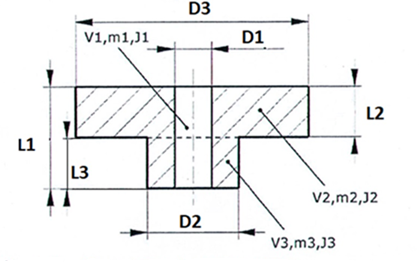
\includegraphics[width=.9\linewidth]{images/flywheel}
	\caption{Эскиз маховика}
	\label{fig:flywheel-sketch}
	\captionsetup{justification=centering}
	\vspace{2mm}
	\small
	\begin{minipage}{.92\linewidth}
		\textit{Обозначения (для расчётов):}
		\(V_1,m_1,J_1\) — объём, масса и момент инерции цилиндра;
		\(V_2,m_2,J_2\) — объём, масса и момент инерции большого диска;
		\(V_3,m_3,J_3\) — объём, масса и момент инерции малого диска.
	\end{minipage}
\end{figure}

Измерения выполняют штангенциркулем ШЦЦ-I-125-0,01
с абсолютной погрешностью \(\pm\SI{0.03}{\milli\meter}\).

\begin{table}[h]
	\centering
	\begin{threeparttable}
		\caption{Результаты измерений геометрических размеров}
		\label{tab:geom}
		\begin{tabular}{@{}lll@{}}
			\toprule
			Обозначение & Значение & Комментарий \\
			\midrule
			\(D_1\) & \SI{11.01}{\milli\meter} & диаметр вала \\
			\(D_2\) & \SI{69.03}{\milli\meter} & диаметр большого диска \\
			\(D_3\) & \SI{26.98}{\milli\meter} & диаметр малого диска \\
			\(L_1\) & \SI{30.04}{\milli\meter} & ширина большого диска \\
			\(L_2\) & \SI{15.08}{\milli\meter} & ширина малого диска \\
			\(L_3\) & \SI{14.96}{\milli\meter} & длина втулки/цилиндра \\
			\bottomrule
		\end{tabular}
	\end{threeparttable}
\end{table}


Измеряют массу маховика взвешиванием на весах EK-12Ki с пределом допускаемой погрешности \SI{\pm 3}{\gram}. масса маховика составляет $\SI{0,488}{\kilogram}$. 

Рассчитывают объём маховика как сумму объёмов составных частей:
\begin{equation}
	 V = V_2 + V_3 - V_1
\end{equation}

Объём одной составной части определяют как:
\begin{equation}
	V_i = \pi \cdot r_i^2 \cdot h_i
\end{equation}
где \(r_i\)--- радиус диска составной части маховика, \(h_i\)"--- высота составной части маховика.

\begin{equation}
 	\begin{aligned}
 		V_1 &= \pi r_1^2 h_1 = 2860 \,\text{мм}^3 = 2.860 \cdot 10^{-6}\,\text{м}^3, \\
 		V_2 &= \pi r_2^2 h_2 = 55972 \,\text{мм}^3 = 5.597 \cdot 10^{-5}\,\text{м}^3, \\
 		V_3 &= \pi r_3^2 h_3 = 8621 \,\text{мм}^3 = 8.552 \cdot 10^{-6}\,\text{м}^3, \\
 		V   &= 6.173 \cdot 10^{-5}\,\text{м}^3.
 	\end{aligned}
\end{equation}

Определяют погрешность измерения объёма:

\begin{equation}
	\begin{aligned}
		\Delta V_i &= V_i \sqrt{
			\left( \frac{\partial \ln(V_i)}{\partial r_i}\Delta r \right)^2 +
			\left( \frac{\partial \ln(V_i)}{\partial h_i}\Delta h \right)^2 }
		= V_i \sqrt{\left(\tfrac{2}{r_i}\Delta r\right)^2 + \left(\tfrac{1}{h_i}\Delta h\right)^2 } \\[1ex]
		\Delta V_1 &= 2860 \sqrt{ \left(\tfrac{2}{5.5}\cdot 0.03\right)^2 + \left(\tfrac{1}{30.04}\cdot 0.03\right)^2 }
		= 3.13 \cdot 10^{-8}\,\text{м}^3 \\[1ex]
		\Delta V_2 &= 55972 \sqrt{ \left(\tfrac{2}{34.515}\cdot 0.03\right)^2 + \left(\tfrac{1}{14.96}\cdot 0.03\right)^2 }
		= 1.48 \cdot 10^{-7}\,\text{м}^3 \\[1ex]
		\Delta V_3 &= 8621 \sqrt{ \left(\tfrac{2}{13.49}\cdot 0.03\right)^2 + \left(\tfrac{1}{15.08}\cdot 0.03\right)^2 }
		= 4.20 \cdot 10^{-8}\,\text{м}^3 \\[1ex]
		\Delta V   &= \sqrt{(\Delta V_1)^2 + (\Delta V_2)^2 + (\Delta V_3)^2}
		= 1.59 \cdot 10^{-7}\,\text{м}^3
	\end{aligned}
\end{equation}



Рассчитывают плотность материала маховика по формуле:
\begin{equation}
\rho = \frac{m}{V} = \frac{0.488}{6.173 \cdot 10^{-5}}
= 7905 \,\si{\kilo\gram\per\cubic\meter}
\end{equation}

Находят погрешность измерения плотности $\rho$:

\begin{equation}
	\begin{alignedat}{2}
		\Delta \rho &= 
		\sqrt{\left( \frac{\partial \ln(\rho)}{\partial m} \, \Delta m \right)^{2} +
			\left( \frac{\partial \ln(\rho)}{\partial V} \, \Delta V \right)^{2}}, \\[1ex]
		\Delta \rho &= 7905 \cdot 
		\sqrt{(0.003)^{2} + (1.59 \cdot 10^{-7})^{2}}
		= 2.37 \cdot 10^{-5}\,\frac{\text{кг}}{\text{м}^3}
	\end{alignedat}
\end{equation}

Определяют массу составных частей маховика по формуле:

\begin{equation}
	\begin{alignedat}{1}
		m_i &= V_i \cdot \rho, \\[1ex]
		m_1 &= 2.860 \cdot 10^{-6} \cdot 7905 = 0.0226 \,\text{кг}, \\[1ex]
		m_2 &= 5.597 \cdot 10^{-5} \cdot 7905 = 0.4424 \,\text{кг}, \\[1ex]
		m_3 &= 8.552 \cdot 10^{-6} \cdot 7905 = 0.0677 \,\text{кг}.
	\end{alignedat}
\end{equation}

Определяют погрешность определения массы составных частей:

\begin{equation}
	\begin{aligned}
		\Delta m_i &= m_i \sqrt{
			\left( \frac{\partial \ln(m_i)}{\partial V_i} \Delta V_i \right)^{2} +
			\left( \frac{\partial \ln(m_i)}{\partial \rho} \Delta \rho \right)^{2}}, \\[1ex]
		\Delta m_1 &= 0.0226 \cdot \sqrt{(3.13 \cdot 10^{-8})^{2} + (2.37 \cdot 10^{-5})^{2}}
		= 5.36 \cdot 10^{-7}\,\text{кг}, \\[1ex]
		\Delta m_2 &= 0.4424 \cdot \sqrt{(1.48 \cdot 10^{-7})^{2} + (2.37 \cdot 10^{-5})^{2}}
		= 1.04 \cdot 10^{-5}\,\text{кг}, \\[1ex]
		\Delta m_3 &= 0.0677 \cdot \sqrt{(1.59 \cdot 10^{-7})^{2} + (2.37 \cdot 10^{-5})^{2}}
		= 1.61 \cdot 10^{-6}\,\text{кг}.
	\end{aligned}
\end{equation}

Определяют момент инерции составных частей маховика по формуле:
\begin{equation}
	\begin{aligned}
		J_i &= \frac{m_i}{2} \, r_i^{2}, \\[1ex]
		J_1 &= \frac{m_1}{2} \, r_1^{2} = 3.42 \cdot 10^{-7}\,\text{кг}\cdot\text{м}^2, \\[1ex]
		J_2 &= \frac{m_2}{2} \, r_2^{2} = 2.63 \cdot 10^{-4}\,\text{кг}\cdot\text{м}^2, \\[1ex]
		J_3 &= \frac{m_3}{2} \, r_3^{2} = 6.20 \cdot 10^{-6}\,\text{кг}\cdot\text{м}^2.
	\end{aligned}
\end{equation}

Определяют погрешность измерения момента инерции составных частей маховика по формуле:

\begin{equation}
	\begin{aligned}
		J_i &= J_i \sqrt{
			\left( \frac{\partial \ln(J_i)}{\partial m_i}\,\Delta m_i \right)^{2} +
			\left( \frac{\partial \ln(J_i)}{\partial r_i}\,\Delta r \right)^{2}}, \\[1ex]
		\Delta J_1 &= J_1 \sqrt{
			\left( \frac{\partial \ln(J_1)}{\partial m_1}\,\Delta m_1 \right)^{2} +
			\left( \frac{\partial \ln(J_1)}{\partial r_1}\,\Delta r \right)^{2}}
		= 3.73 \cdot 10^{-9}\,\text{кг}\cdot\text{м}^2, \\[1ex]
		\Delta J_2 &= J_2 \sqrt{
			\left( \frac{\partial \ln(J_2)}{\partial m_2}\,\Delta m_2 \right)^{2} +
			\left( \frac{\partial \ln(J_2)}{\partial r_2}\,\Delta r \right)^{2}}
		= 4.58 \cdot 10^{-7}\,\text{кг}\cdot\text{м}^2, \\[1ex]
		\Delta J_3 &= J_3 \sqrt{
			\left( \frac{\partial \ln(J_3)}{\partial m_3}\,\Delta m_3 \right)^{2} +
			\left( \frac{\partial \ln(J_3)}{\partial r_3}\,\Delta r \right)^{2}}
		= 2.75 \cdot 10^{-8}\,\text{кг}\cdot\text{м}^2.
	\end{aligned}
\end{equation}

Итоговая погрешность составляет:
\begin{equation}
	\Delta J = \sqrt{ (\Delta J_1)^2 + (\Delta J_2)^2 + (\Delta J_3)^2 }
	= 4.58 \cdot 10^{-7}\,\text{кг}\cdot\text{м}^2
\end{equation}

 

\clearpage
\refstepcounter{chapter}


        % Приложения

\setcounter{totalappendix}{\value{chapter}} % Подсчёт количества приложений

\end{document}
